% !TeX encoding = UTF-8
% !TeX program = xelatex
% !TeX spellcheck = en_US

\documentclass[degree=master,language=chinese,font=external,cjk-font=external]{sustechthesis}
  %%%%%%%%%%%%%%%%%%%%%%%%%%%%%%%%%%%%%%%
  %   研究生报告模板:开题报告,年度考核报告
  %%%%%%%%%%%%%%%%%%%%%%%%%%%%%%%%%%%%%%%

  % 学位 degree:
  %   master (默认) | doctor
  % 语言 language:
  %   chinese (默认)| english
  % 英文字体 font
  %   auto (默认,自动选择系统自带字体)| external (包内字体)| times | termes | 等
  %   Windows 和 macOS 系统上,无需设定。系统自带对应字体,可以删除该参数。
  %   Unix 系统推荐使用包内字体,而非TeX自带的克隆版字体,以达到和其他系统一致的字体效果。
  %   Windows 系统上可以删除该参数,使用系统内置字体。
  % 中文字体 cjk-font
  %   auto (默认,自动选择系统自带字体)| external (包内字体)| windows | mac | 等
  %   在 **非Windows** 的系统上推荐使用包内字体,而非系统字体。
  %   以达到和 Windows 系统一致的字体效果。
  %   Windows 系统自带对应字体,可以删除该参数。

  
% 论文基本配置,加载宏包等全局配置
% 在此文件中可以选择
% 1. 【重要】文档类型(开题报告,年度考核报告),默认不开启该选项。
% 2. 生成的PDF为无空白页的用于电子版提交的版本 或 插入空白页的以便双面打印的版本
% 3. 学位学科门类(理学、工学、医学)
% 4. 培养单位
% 5. 作者姓名、指导教师等
% !TeX root = ./sustechthesis-example.tex

% 论文基本信息配置

\thusetup{
  %******************************
  % 注意:
  %   1. 配置里面不要出现**空行**
  %   2. 不需要的配置信息可以删除
  %   3. 建议先阅读文档中所有关于选项的说明
  %******************************
  %
  % 输出格式
  %   选择打印版(print)或用于提交的电子版(electronic),前者会插入空白页以便直接双面打印
  %
  output = print,
  %
  % 文档类型
  %   选择开题报告(proposal)、年度考核报告(progress)或学位论文(thesis)【默认值】。
  %
  type = thesis,
  %
  % 标题
  %   可使用“\\”命令手动控制换行
  %   如果需要使用副标题,取消 subtitle 和 subtitle* 的注释即可。
  %   特别字符允许小写,例如行内公式,其他所有字词全部大写。
  %
  title  = {弹性蛇形条带的分岔和稳定性分析及其后屈曲行为的调控},
  title* = {Bifurcation and Stability Analysis of Elastic Serpentine Strips and tuning of their Post-Buckling Response},
  % subtitle = {可选的副标题可选的副标题可选的副标题可选的副标题可选的副标题可选的副标题},
  % subtitle* = {optional subtitle optional subtitle optional subtitle optional subtitle optional subtitle optional subtitle},
  %
  % 学位
  %
  degree-domain = {工学}, % 【中文】学科门类:可选理学、工学、医学
  degree-domain* = {Engineering}, % 【英文】学位等级:可选Science, Engineering, Medicine
  degree-type = {academic},  % 学位类型:可选学术型(academic)【默认值】、专业型(professional)。
  %
  % 培养单位
  %   填写所属院系的全名
  %   超长英文系名可以手动换行
  department = {力学与航空航天工程系},
  department* = {College of Engineering},
  %
  % 学科
  %   1. 学术型学位
  %      获得一级学科授权的学科填写一级学科名称,其他填写二级学科名称
  %   2. 工程硕士
  %      工程领域名称
  %
  discipline  = {力学},
  discipline* = {Mechanics},
  %
  % 姓名
  %   英文用全拼,姓在前,名在后,姓和名的首字母大写,其余小写
  %
  author-id  = {12232461},
  author  = {师启耀},
  author* = {Shi Qiyao},
  %
  % 指导教师
  %   一般情况下,只写一名指导教师。
  %   填写导师姓名,后衬导师职称“教授”,“副教授”,“研究员”等
  %
  supervisor  = {李明武},
  supervisor* = {Assistant Prof. Li Mingwu},
  % 副指导教师
  %   一般无需启用该项,留空或者注释掉即可。
  %   如需启用限填写一名,且需要向学位办确认和备案,职称要求同指导教师。
  % associate-supervisor  = {大卫查理助理教授},
  % associate-supervisor* = {Assistant Prof. David Charlie},
  %
  % 日期
  %   使用 ISO 格式;默认为当前时间
  %   date 为第一页全中文大写日期,defense-date 为第二、三页的答辩日期。
  %   需要按 {年-月-日} 格式填写,如不显示“日”,可以随意填一个日期,但是不能为空。
  %
  date = {2025-5-7},
  defense-date = {2025-5-20},
  %
  % 密级
  %   公开, 秘密, 机密, 绝密
  %
  statesecrets={公开},
  %
  % 国内图书分类号:查询网址:https://ztflh.xhma.com/
  %   国内图书分类号可先参考知网上类似学位论文的分类号,再进行确认。
  % 国际图书分类号,查询网址:https://udcsummary.info/php/index.php?lang=chi
  %
  natclassifiedindex={O342},
  intclassifiedindex={531},
}
%\usepackage{amssymb}
%\usepackage{unicode-math}
%\thusetup{
%  %
%  % 数学字体
%  % math-style = GB,  % GB (中文默认) | TeX (英文默认)
%  math-font  = cambria,  % cambria (默认,同 Word 默认数学字体一致) | times (Times New Roman 的TeX克隆版)| xits | stix
%}

% 载入所需的宏包

% 可以使用 nomencl 生成符号和缩略语说明
% \usepackage{nomencl}
% \makenomenclature

% 表格加脚注
\usepackage{threeparttable}

% 表格中支持跨行
\usepackage{multirow}

% 量和单位
\usepackage{siunitx}

% 定理类环境宏包
\usepackage{amsthm}
% 也可以使用 ntheorem
% \usepackage[amsmath,thmmarks,hyperref]{ntheorem}
\usepackage{tikz}
\newcommand{\bluesquare}{\tikz{\fill[blue] (0,0) rectangle (0.25,0.25);}}
\newcommand{\blacksquare}{\tikz{\fill[black] (0,0) rectangle (0.25,0.25);}}
\newcommand{\redsquare}{\tikz{\fill[red] (0,0) rectangle (0.25,0.25);}}
\newcommand{\Rlefttriangle}{\tikz\fill[red] (0,0) -- (-0.3,0.15) -- (-0.3,-0.15) -- cycle;}
\newcommand{\Rrighttriangle}{\tikz\fill[red] (0,0) -- (0.3,0.15) -- (0.3,-0.15) -- cycle;}
\newcommand{\Blefttriangle}{\tikz\fill[blue] (0,0) -- (-0.3,0.15) -- (-0.3,-0.15) -- cycle;}
\newcommand{\Brighttriangle}{\tikz\fill[blue] (0,0) -- (0.3,0.15) -- (0.3,-0.15) -- cycle;}
\newcommand{\Btriangle}{\tikz\fill[blue] (0,0) -- (0.15,0.3) -- (0.3,0) -- cycle;}
\newcommand{\Rtriangle}{\tikz\fill[red] (0,0) -- (0.15,0.3) -- (0.3,0) -- cycle;}
\newcommand{\bltriangle}{\tikz\fill[black] (0,0) -- (0.15,0.3) -- (0.3,0) -- cycle;}
%\newcommand{\redtriangle}{\tikz\fill[red] (0,0) -- (0.15,0.3) -- (0.3,0) -- cycle;}

\newcommand{\Rdiamond}{\tikz\draw[fill=red, draw=red,scale=0.2] (0,0) -- (0.5,0.866) -- (1,0) -- (0.5,-0.866) -- cycle;}
\newcommand{\Bdiamond}{\tikz\draw[fill=blue, draw=blue,scale=0.2] (0,0) -- (0.5,0.866) -- (1,0) -- (0.5,-0.866) -- cycle;}
\newcommand{\blackdiamond}{\tikz\draw[fill=black, draw=black,scale=0.2] (0,0) -- (0.5,0.866) -- (1,0) -- (0.5,-0.866) -- cycle;}
\newcommand{\HRlefttriangle}{\tikz\draw[draw=red] (0,0) -- (-0.3,0.15) -- (-0.3,-0.15) -- cycle;}
\newcommand{\HRrighttriangle}{\tikz\draw[draw=red] (0,0) -- (0.3,0.15) -- (0.3,-0.15) -- cycle;}
\newcommand{\HBlefttriangle}{\tikz\draw[draw=blue](0,0) -- (-0.3,0.15) -- (-0.3,-0.15) -- cycle;}
\newcommand{\HBrighttriangle}{\tikz\draw[draw=blue] (0,0) -- (0.3,0.15) -- (0.3,-0.15) -- cycle;}
\newcommand{\Bstarshape}{\tikz\draw[fill=blue, draw=blue,scale=0.2] (0,1) 
	-- (0.225, 0.309) -- (1, 0.309) 
	-- (0.381, -0.118) -- (0.618, -0.809) 
	-- (0, -0.381) -- (-0.618, -0.809) 
	-- (-0.381, -0.118) -- (-1, 0.309) 
	-- (-0.225, 0.309) -- cycle;}
\newcommand{\Rstarshape}{\tikz\draw[fill=red, draw=red,scale=0.2] (0,1) 
		-- (0.225, 0.309) -- (1, 0.309) 
		-- (0.381, -0.118) -- (0.618, -0.809) 
		-- (0, -0.381) -- (-0.618, -0.809) 
		-- (-0.381, -0.118) -- (-1, 0.309) 
		-- (-0.225, 0.309) -- cycle;}
\makeatletter
\newcommand*{\rom}[1]{\expandafter\@slowromancap\romannumeral #1@}
\makeatother

%%%%%% 顺序编码制的文献引用形式
%%%%%% 参考文献编译方式二选一,不要同时开启。
%%%% 选择一:使用 BibTeX + natbib 宏包
\usepackage[sort&compress]{natbib}
% 全局上标数字模式
\bibliographystyle{sustechthesis-numeric}
% 全局著者-出版年制模式
% \bibliographystyle{sustechthesis-author-year}

%%%% 选择二:使用 BibLaTeX 宏包(兼容性不佳,不太推荐)
% 全局上标数字模式
% \usepackage[backend=biber,style=gb7714-2015,gbalign=left]{biblatex}
% 全局著者-出版年制模式
% \usepackage[backend=biber,style=gb7714-2015ay]{biblatex}
% \addbibresource{ref/refs.bib} % 声明 BibLaTeX 的数据库

% 定义所有的图片文件在 figures 子目录下
\graphicspath{{figures/}}

% \enabledraftmode % 启用图片草稿模式,会以文字占位符替代图片,加快大量插入大尺寸图片时的编译速度,用于学位论文的调试,默认不启用

% 数学命令
\newcommand\dif{\mathop{}\!\mathrm{d}}  % 微分符号


% hyperref 宏包在最后调用
\usepackage{hyperref}
\usepackage{ragged2e}

% 固定宽度的表格。放在 hyperref 之前的话,tabularx 里的 footnote 显示不出来。
\usepackage{tabularx}

% 跨页表格,必须在 hyperref 之后使用否则会报错。
\usepackage{longtable}

% % 源代码 minted 高亮,二选一即可。【不再推荐,会有兼容性问题:导致图表间距异常】
% %% 使用 minted 包有内置高亮颜色,需要 Python 环境编译,并安装 Pygement 包。
% \usepackage{minted}

% 源代码 listings 高亮,二选一即可。
\usepackage{listings}
%% 使用 listings 包需要自行定义高亮颜色,此处给出 Java 的例子。
\definecolor{javared}{rgb}{0.6,0,0} % for strings
\definecolor{javagreen}{rgb}{0.25,0.5,0.35} % comments
\definecolor{javapurple}{rgb}{0.5,0,0.35} % keywords
\definecolor{javadocblue}{rgb}{0.25,0.35,0.75} % javadoc

\lstset{language=Java,
  keywordstyle=\color{javapurple}\bfseries,
  stringstyle=\color{javared},
  commentstyle=\color{javagreen},
  morecomment=[s][\color{javadocblue}]{/**}{*/},
  numbers=left,
  numberstyle=\tiny\color{black},
  stepnumber=1,
  numbersep=10pt,
  tabsize=4,
  showspaces=false,
  showstringspaces=false
}

% 伪代码环境
\usepackage[ruled,linesnumbered]{algorithm2e}
% 定义伪代码的continue
\SetKw{Continue}{continue}
\SetKw{Break}{break}
% 定义算法注释
\SetKwComment{Comment}{/* }{ */}
\SetKwComment{SingleComment}{// }{}
\SetKwComment{TriComment}{$\triangleright$\ }{}

% tabular 扩展命令
\newcolumntype{R}[1]{>{\raggedleft\arraybackslash}p{#1}} % 定义R为表格左右居左,用于自定义表格列宽度
\newcolumntype{L}[1]{>{\raggedright\arraybackslash}p{#1}} % 定义L为表格左右居右,用于自定义表格列宽度
\newcolumntype{C}[1]{>{\centering\arraybackslash}p{#1}} % 定义C为表格左右居中,用于自定义表格列宽度

% tabularx 扩展命令,会对单元格内容进行单元格内自动换行
% X 默认就是两端对齐
% Y 左对齐
\newcolumntype{Y}{>{\raggedright\arraybackslash}X}
% Z 右对齐
\newcolumntype{Z}{>{\raggedleft\arraybackslash}X}
% A 居中对齐
\newcolumntype{A}{>{\centering\arraybackslash}X}


\begin{document}

% 封面
\maketitle

\frontmatter

% 目录
\tableofcontents

% 插图和附表清单
% \listoffiguresandtables  % 插图和附表清单
% \listoffigures           % 插图清单
% \listoftables            % 附表清单

% 符号对照表(非强制性要求,如果论文中所用符号不多,可以略去)
% % !TeX root = ../sustechthesis-example.tex

% denotation 环境带一个可选参数,用来指定符号列的宽度(默认为 2.5cm),下面改3cm为例。
% 如果论文中使用了大量的物理量符号、标志、缩略词、专门计量单位、自定义名词和术语等, 应编写“符号和缩略语说明”。
% 论文中主要符号应全部采用法定单位, 严格执行《量和单位》(GB3100~3102-93)的有关规定、单位名称的书写,可以采用国际通用符号,也可以用中文名称,但全文应统一,不得两种混用。
% 缩略语应列出中英文全称。符号和缩略语说明排序方法先按拉丁字母大写、小写排序, 再按希腊字母大写、小写排序, 如下表所示:
% ABCDEFGHIJKLMNOPQRSRUVWXYZ
% abcdefghijklmnopqrstuvwxyz
% Alpha
% Beta
% Gamma
% Delta
% Epsilon
% Zeta
% Eta
% Theta
% Iota
% Kappa
% Lambda
% Mu
% Nu
% Xi
% Omicron
% Pi
% Rho
% Sigma
% Tau
% Upsilon
% Phi
% Chi
% Psi
% Omega
% alpha
% beta
% gamma
% delta
% epsilon
% zeta
% eta
% theta
% iota
% kappa
% lambda
% mu
% nu
% xi
% omicron
% pi
% rho
% sigma
% tau
% upsilon
% phi
% chi
% psi
% omega

% 希腊字母详见 https://xilazimu.net/


\begin{denotation}[3cm]
  \item[As-PPT]聚苯基不对称三嗪
  \item[DFT]密度泛函理论 (Density Functional Theory)
  \item[DMAsPPT]聚苯基不对称三嗪双模型化合物(水解实验模型化合物)
  \item[$E_a$]化学反应的活化能 (Activation Energy)
  \item[HMAsPPT]聚苯基不对称三嗪模型化合物的质子化产物
  \item[HMPBI]聚苯并咪唑模型化合物的质子化产物
  \item[HMPI]聚酰亚胺模型化合物的质子化产物
  \item[HMPPQ]聚苯基喹噁啉模型化合物的质子化产物
  \item[HMPY]聚吡咙模型化合物的质子化产物
  \item[HMSPPT]聚苯基对称三嗪模型化合物的质子化产物
  \item[HPCE]高效毛细管电泳色谱 (High Performance Capillary lectrophoresis)
  \item[HPLC]高效液相色谱 (High Performance Liquid Chromatography)
  \item[IRC]内禀反应坐标 (Intrinsic Reaction Coordinates)
  \item[LC-MS]液相色谱-质谱联用 (Liquid chromatography-Mass Spectrum)
  \item[MAsPPT]聚苯基不对称三嗪单模型化合物,3,5,6-三苯基-1,2,4-三嗪
  \item[MPBI]聚苯并咪唑模型化合物,N-苯基苯并咪唑
  \item[MPI]聚酰亚胺模型化合物,N-苯基邻苯酰亚胺
  \item[MPPQ]聚苯基喹噁啉模型化合物,3,4-二苯基苯并二嗪
  \item[MPY]聚吡咙模型化合物
  \item[MSPPT]聚苯基对称三嗪模型化合物,2,4,6-三苯基-1,3,5-三嗪
  \item[ONIOM]分层算法 (Our own N-layered Integrated molecular Orbital and molecular Mechanics)
  \item[PBI]聚苯并咪唑
  \item[PDT]热分解温度
  \item[PES]势能面 (Potential Energy Surface)
  \item[PI]聚酰亚胺
  \item[PMDA-BDA]均苯四酸二酐与联苯四胺合成的聚吡咙薄膜
  \item[PPQ]聚苯基喹噁啉
  \item[PY]聚吡咙
  \item[S-PPT]聚苯基对称三嗪
  \item[SCF]自洽场 (Self-Consistent Field)
  \item[SCRF]自洽反应场 (Self-Consistent Reaction Field)
  \item[TIC]总离子浓度 (Total Ion Content)
  \item[TS]过渡态 (Transition State)
  \item[TST]过渡态理论 (Transition State Theory)
  \item[ZPE]零点振动能 (Zero Vibration Energy)
  \item[\textit{ab initio}]基于第一原理的量子化学计算方法,常称从头算法
  \item[$\Delta G^\neq$]活化自由能(Activation Free Energy)
  \item[$\kappa$]传输系数 (Transmission Coefficient)
  \item[$\nu_i$]虚频 (Imaginary Frequency)
\end{denotation}



% 也可以使用 nomencl 宏包,需要在导言区
% \usepackage{nomencl}
% \makenomenclature

% 在这里输出符号说明
% \printnomenclature[3cm]

% 在正文中的任意为都可以标题
% \nomenclature{As-PPT}{聚苯基不对称三嗪}
% \nomenclature{DFT}{密度泛函理论 (Density Functional Theory)}
% \nomenclature{DMAsPPT}{聚苯基不对称三嗪双模型化合物(水解实验模型化合物)}
% \nomenclature{$E_a$}{化学反应的活化能 (Activation Energy)}
% \nomenclature{HMAsPPT}{聚苯基不对称三嗪模型化合物的质子化产物}
% \nomenclature{HMPBI}{聚苯并咪唑模型化合物的质子化产物}
% \nomenclature{HMPI}{聚酰亚胺模型化合物的质子化产物}
% \nomenclature{HMPPQ}{聚苯基喹噁啉模型化合物的质子化产物}
% \nomenclature{HMPY}{聚吡咙模型化合物的质子化产物}
% \nomenclature{HMSPPT}{聚苯基对称三嗪模型化合物的质子化产物}
% \nomenclature{HPCE}{高效毛细管电泳色谱 (High Performance Capillary lectrophoresis)}
% \nomenclature{HPLC}{高效液相色谱 (High Performance Liquid Chromatography)}
% \nomenclature{IRC}{内禀反应坐标 (Intrinsic Reaction Coordinates)}
% \nomenclature{LC-MS}{液相色谱-质谱联用 (Liquid chromatography-Mass Spectrum)}
% \nomenclature{MAsPPT}{聚苯基不对称三嗪单模型化合物,3,5,6-三苯基-1,2,4-三嗪}
% \nomenclature{MPBI}{聚苯并咪唑模型化合物,N-苯基苯并咪唑}
% \nomenclature{MPI}{聚酰亚胺模型化合物,N-苯基邻苯酰亚胺}
% \nomenclature{MPPQ}{聚苯基喹噁啉模型化合物,3,4-二苯基苯并二嗪}
% \nomenclature{MPY}{聚吡咙模型化合物}
% \nomenclature{MSPPT}{聚苯基对称三嗪模型化合物,2,4,6-三苯基-1,3,5-三嗪}
% \nomenclature{ONIOM}{分层算法 (Our own N-layered Integrated molecular Orbital and molecular Mechanics)}
% \nomenclature{PBI}{聚苯并咪唑}
% \nomenclature{PDT}{热分解温度}
% \nomenclature{PES}{势能面 (Potential Energy Surface)}
% \nomenclature{PI}{聚酰亚胺}
% \nomenclature{PMDA-BDA}{均苯四酸二酐与联苯四胺合成的聚吡咙薄膜}
% \nomenclature{PPQ}{聚苯基喹噁啉}
% \nomenclature{PY}{聚吡咙}
% \nomenclature{S-PPT}{聚苯基对称三嗪}
% \nomenclature{SCF}{自洽场 (Self-Consistent Field)}
% \nomenclature{SCRF}{自洽反应场 (Self-Consistent Reaction Field)}
% \nomenclature{TIC}{总离子浓度 (Total Ion Content)}
% \nomenclature{TS}{过渡态 (Transition State)}
% \nomenclature{TST}{过渡态理论 (Transition State Theory)}
% \nomenclature{ZPE}{零点振动能 (Zero Vibration Energy)}
% \nomenclature{\textit{ab initio}}{基于第一原理的量子化学计算方法,常称从头算法}
% \nomenclature{$\Delta G^\neq$}{活化自由能(Activation Free Energy)}
% \nomenclature{$\kappa$}{传输系数 (Transmission Coefficient)}
% \nomenclature{$\nu_i$}{虚频 (Imaginary Frequency)}



% 正文部分
\mainmatter
% !TeX root = ../sustechthesis-example.tex

\chapter{引\quad 言}
\section{研究背景与意义}
细长杆、薄板薄壳等结构在外载荷作用下会发生结构失稳屈曲\cite{BAZANT200055,bazant2010stability}。在传统意义上,结构失稳被视为一种需要避免的现象,因为失稳通常意味着结构的失效、功能丧失甚至灾难性后果。例如,在建筑工程中,梁杆的屈曲失稳可能导致建筑物,桥梁的坍塌;在航空航天领域,机翼或壳体的失稳可能引发飞行事故。

对于细长结构和薄壁结构,在载荷作用下往往可以发生很大的位移以及旋转,同时其应变仍保持小应变状态,即结构在展现出明显的几何非线性的同时材料保持在线性范围且不发生失效。当此类柔性结构处于后屈曲阶段时,往往展示出了丰富的非线性行为,如多稳态行为及不同稳态构形之间的突跳行为。基于此,近年来研究者开始将这类柔性结构的失稳行为视为设计具有新型功能结构的机会,而非结构发生失效破坏的源头\cite{10.1115/1.4031456}。通过对结构精确设计和控制失稳行为,从而赋予结构全新的力学特性,如利用柔性结构的后屈曲行为来设计展开结构,自适应结构,超材料,柔性机器人以及将其应用于柔性电子设备中。

近年来,研究者们在利用结构失稳实现新特性方面取得了一系列重要进展,如图~\ref{fig:1}所示。在结构设计领域,研究者利用结构的后屈曲特性来设计展开结构,发展自适应结构。展开结构的初始构形通常为高度紧致的折叠状态。在外部激励(如机械力、热激励或电激励)的作用下,这些结构能够通过特定的变形机制从二维平面状态或紧凑的三维状态转变为大尺度的空间三维构形。其中一种展开方式为处于平面二维状态的结构在受到特定的外力时会产生面外屈曲,从而展开为三维构形\cite{panetta2019x,chen2021bistable,liu2023deployable,10.1145/3386569.3392490,yu2023continuous}。
自适应结构能够根据载荷条件的变化,自动调整形态与行为,来优化其性能或维持功能。例如,在航空领域一些研究者利用复合材料来制造多稳态翼型,这些翼型可以自主切换构形来适应不同的气动载荷\cite{arrieta2013modelling,DIACONU2008689}。由于这些结构具有轻量化,智能化(可自适应外界条件)等特点,因此被广泛应用于各种工程领域,如航空航天\cite{zhang2021deployable},土木建筑\cite{GEIGER20208363}。
在超材料(metamaterials)领域,通过设计周期性微结构并利用其失稳行为,可以实现负泊松比、负刚度和可编程力学性能等奇异特性\cite{cui2014coding}。这些超材料在冲击防护、振动隔离和能量吸收等方面展现出巨大的应用潜力。
在机器人设计领域,一些微小型机器人利用柔性结构的突跳行为来为机器人提供驱动力,例如双稳态结构在两个稳态之间的突跳可以为游泳机器人提供动力\cite{chen2018harnessing,chi2022snapping}。
\begin{figure}
	\centering
	\subcaptionbox{展开结构\cite{10.1145/3386569.3392490}\label{fig:1_1}}
	{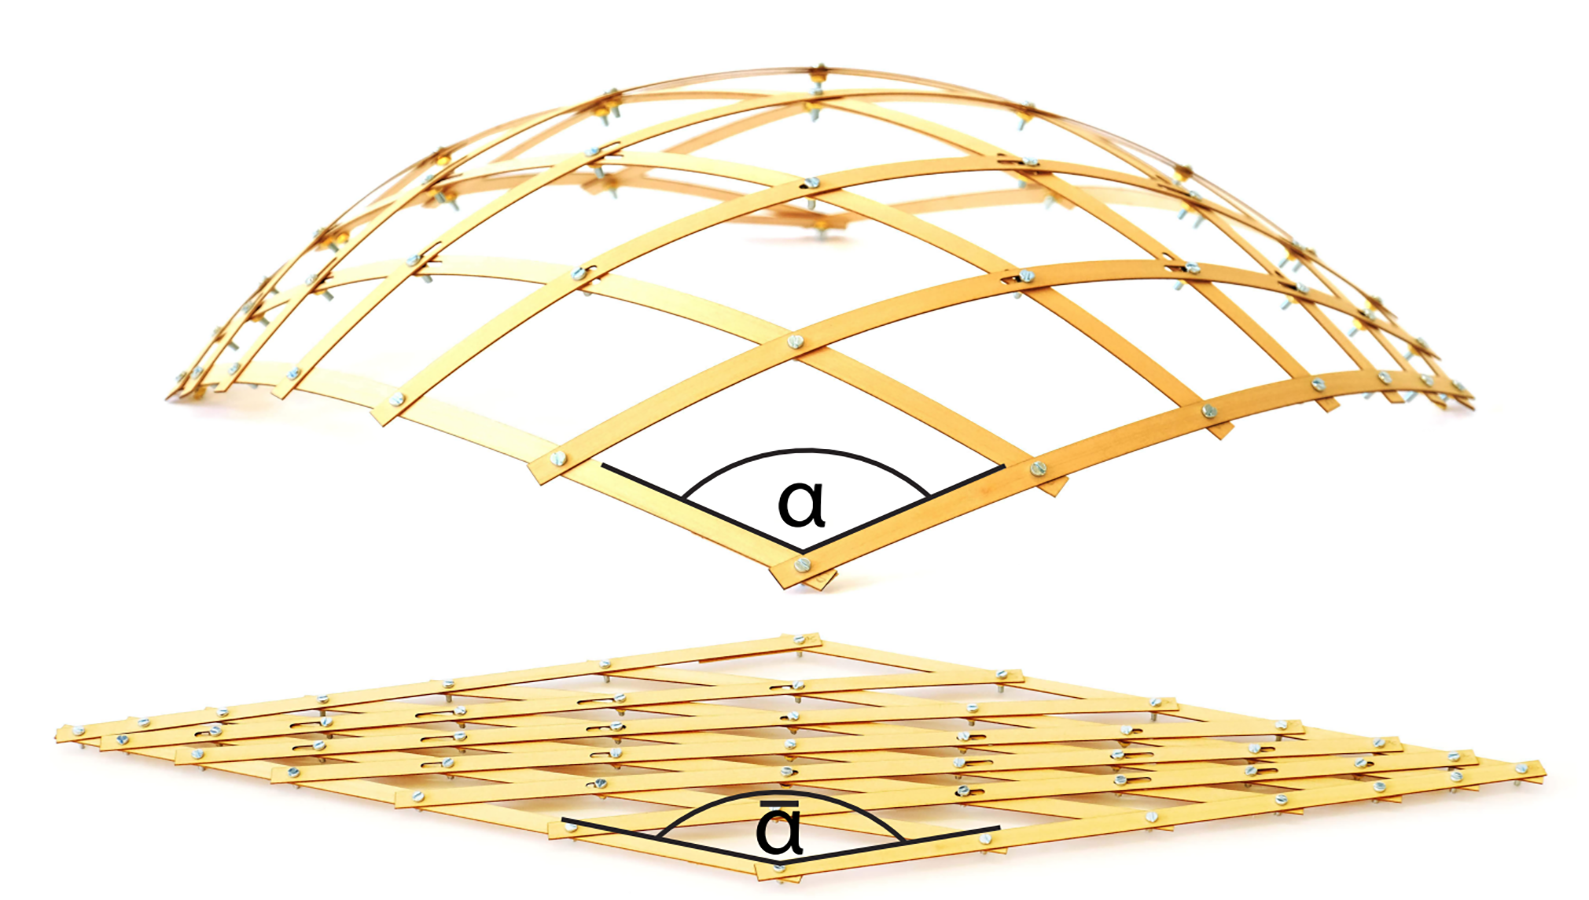
\includegraphics[width=0.49\linewidth]{1_1(1).png}}
	\subcaptionbox{不同载荷下的二维格状蜂窝超材料\cite{PhysRevLett.99.084301}\label{fig:1_2}}
	{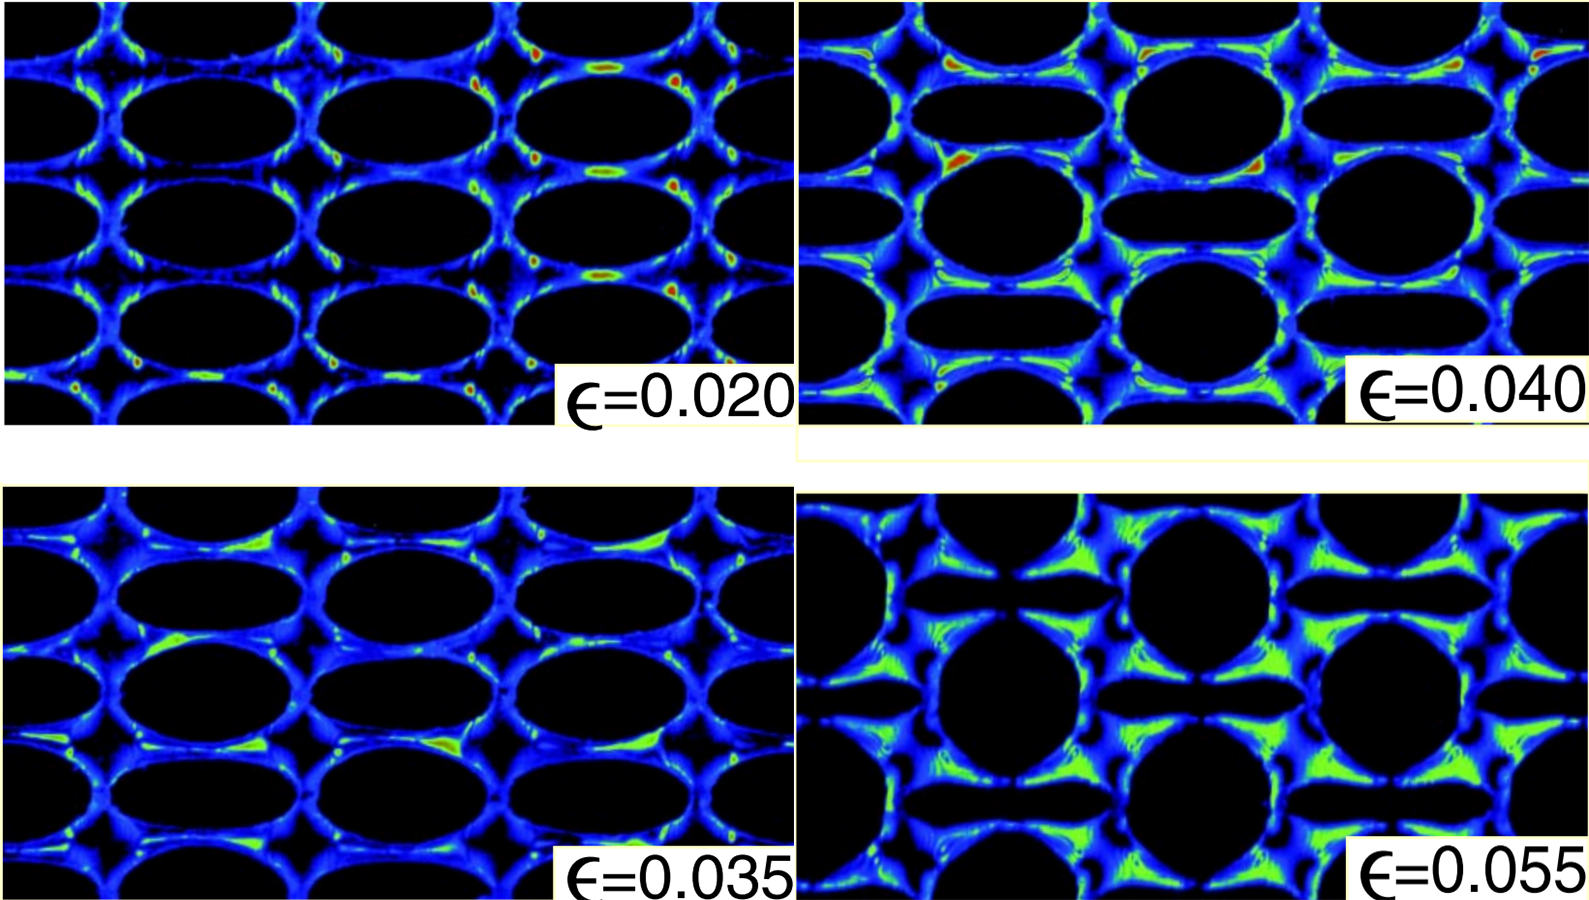
\includegraphics[width=0.49\linewidth]{1_1(2).png}}\\
	\subcaptionbox{双稳态负泊松比结构\cite{chen2021bistable}\label{fig:1_3}}
	{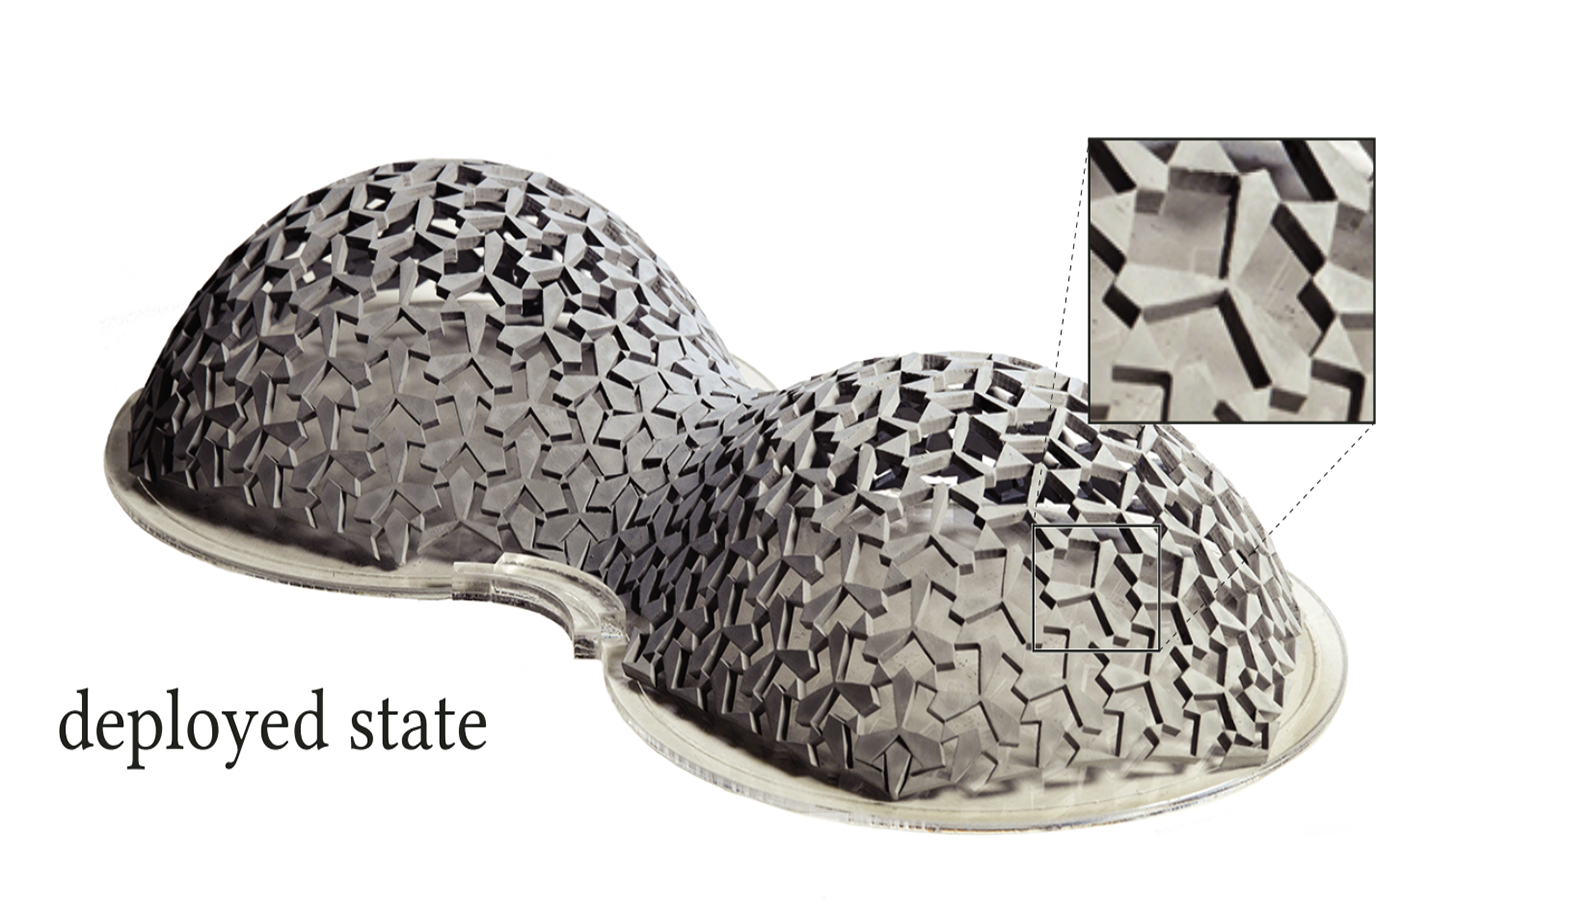
\includegraphics[width=0.49\linewidth]{1_1(3).png}}
	\subcaptionbox{无系链游泳机器人\cite{chen2018harnessing}\label{fig:1_4}}
	{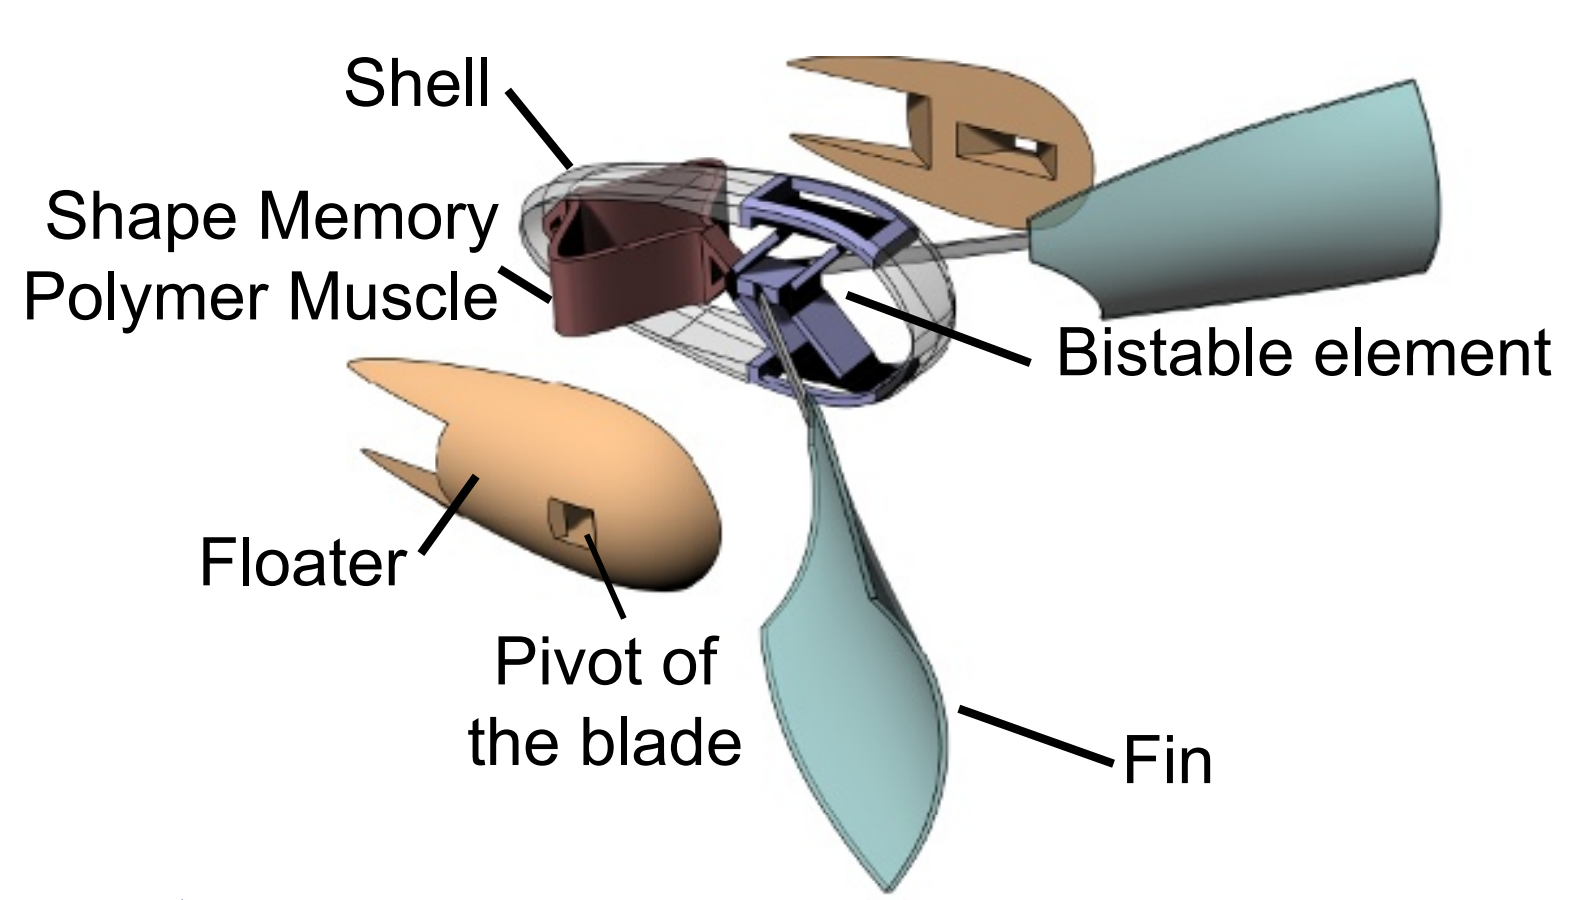
\includegraphics[width=0.49\linewidth]{1_1(4).png}}
	\caption{结构失稳在展开结构,超材料以及机器人领域的应用}
	\label{fig:1}
\end{figure}

另一方面,对柔性结构的屈曲失稳研究为柔性电子设备的设计与制造提供了力学基础。相比于传统的电子设备,柔性电子设备可以更好的贴合复杂曲面以及进行动态变形来适应不同的应用场景,此外柔性电子设备往往使用超薄材料来设计,因此具有轻质化和薄型化的特点。基于上述特点与优势,柔性电子设备展现出了越来越重要的应用前景,包括可穿戴的通讯系统,佩戴式健康监测设备,可嵌入人体的治疗疾病设备,机器人柔性皮肤\cite{rogers2010materials}等。为了制造这些柔性电子设备,近年来发展了许多重要技术,其中平面印刷技术\cite{yin2020structural}(planar printing techniques)通过利用结构的屈曲失稳行为来制备柔性电子设备,该技术由于其相对于其他技术的简单性而被广泛应用。平面印刷技术大致可以分为三类:基底设计技术,三维组装技术,蛇形设计与岛桥结构。

在基底设计技术\cite{bowden1998spontaneous}中,首先对柔软基底进行预处理(如拉伸或加热处理)以在基底中引入预应力。随后,将电子器件安置在预处理后的柔性基底上。当基底释放预应力时,基底自身的变形会对电子器件施加压力,导致电子器件发生面外屈曲,形成稳定的褶皱形貌。这种褶皱结构为结构提供了更多可拉伸空间,从而显著增强了电子设备的可拉伸性和机械耐久性。相比之下,三维组装技术则更为复杂,需要对基底进行精确加工以实现特定的预应力分布,并通过精确设计电子器件的二维初始构形及其与基底的粘接区域,将二维电子器件转换为目标三维构形\cite{cheng2023programming}。这种技术不仅依赖于基底的力学特性,还需要对器件的几何形状和材料性能进行精细调控,以实现复杂的三维结构。“岛—桥”结构\cite{zhang2013buckling},如图~\ref{fig:1_2v}所示,为柔性电子设备制造的另外一类方法。该方法中,整个电子设备被安置到可变形的基底上,在基底上排布一系列小的刚性底片(island)用以布置设备的主要部件,并将每个小的刚性底片利用可承受较大变形的连接部件(bridge)进行连接,实现不同基底之间的通信和电传导。对于这一类布局,其用以安装电子功能元器件的小刚片单元往往为刚性结构,整个设备的可拉伸性取决于连接部件的可拉伸性,其中一种被广泛应用于柔性电子的连接部件为蛇形结构\cite{li2005compliant},如图~\ref{fig:1_2v}中下方黑色曲线所示。
\begin{figure}
	\centering
	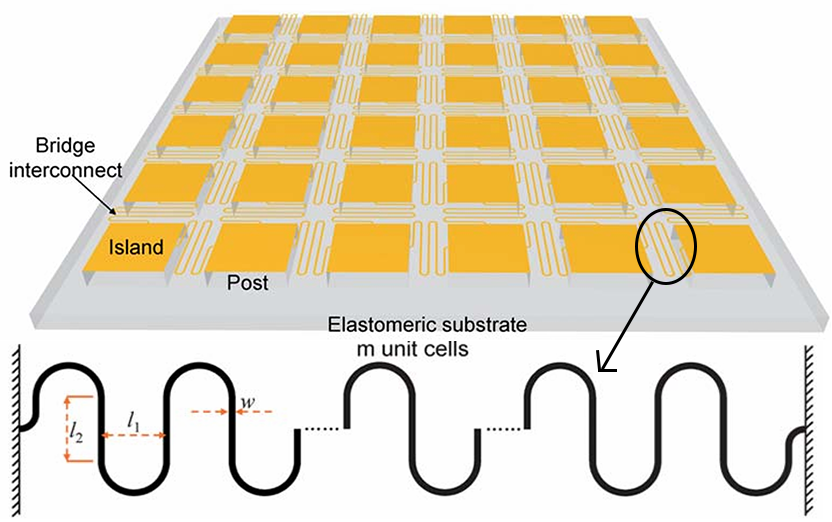
\includegraphics[width=0.6\linewidth]{1_2v.png}
	\caption{“岛—桥”布局及蛇形结构\cite{zhang2013buckling}}
	\label{fig:1_2v}
\end{figure}

蛇形结构是由若干蛇形单元构成,每一蛇形单元由直线条带与半圆弧条带相互交错连接而成\cite{li2005compliant}。相比于直线条带,蛇形条带具有更好的可拉伸性。由于蛇形条带的截面宽度远大于其厚度,面外弯曲刚度远小于平面内弯曲刚度,因此当拉伸载荷超过某一临界值时结构会发生面外屈曲。而在后屈曲阶段,蛇形结构的弹性能主要是由弯曲和扭转弹性能为主,保证了在较大拉伸下蛇形结构不会因轴向拉伸而破坏。正因为蛇形结构良好的可拉伸性,该结构已被广泛应用于各类柔性器件中,如图~\ref{fig:1_3v}所示。例如,Jiao等\cite{jiao2023vertical}通过蛇形结构连接各个电子器件来构建曲面型的电子设备;Kobayashi等\cite{Kobayashi2018FlexibleSW}通过采用蛇形条带将超薄芯片与基座连接,实现了芯片在基座上的可移动性,使芯片能够在基座上进行有限范围内的位移或旋转。Xu等\cite{xu2013stretchable}利用蛇形结构连接电池单元来制造可拉伸柔性电池。Lai等\cite{lai2017single}将可穿戴式摩擦发电单元设计为蛇形结构并安置在编织基底上,提高了该能量收集装置的可拉伸性。
\begin{figure}
	\centering
	\subcaptionbox{曲面型柔性电子设备\cite{jiao2023vertical}\label{fig:1_3(1)}}
	{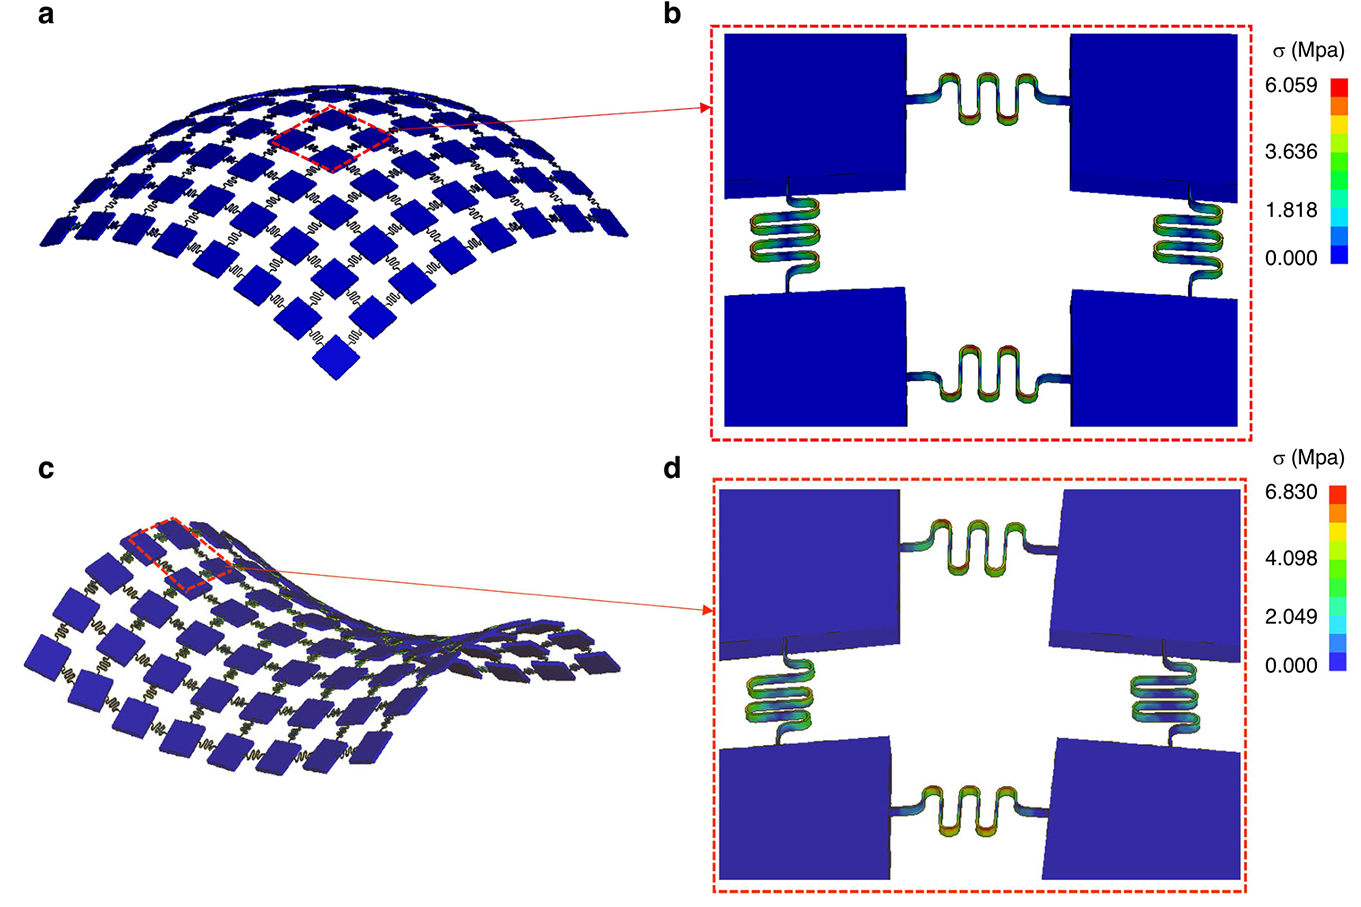
\includegraphics[width=0.45\linewidth]{1_3(3).png}}
	\subcaptionbox{可移动芯片基座\cite{PhysRevLett.99.084301}\label{fig:1_3(2)}}
	{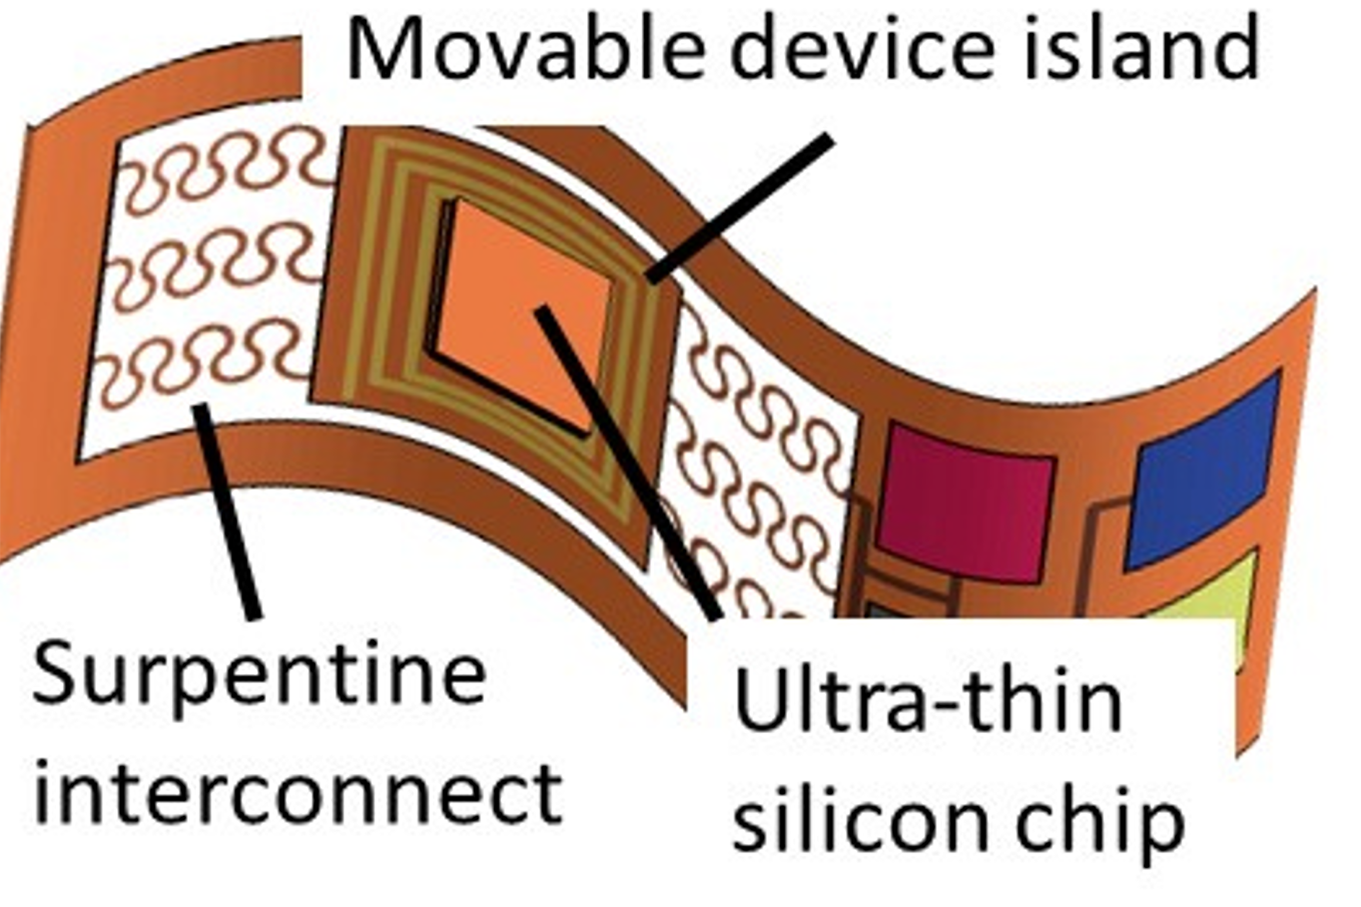
\includegraphics[width=0.45\linewidth]{1_3(4).png}}\\
	\subcaptionbox{柔性电池\cite{xu2013stretchable}\label{fig:1_3(3)}}
	{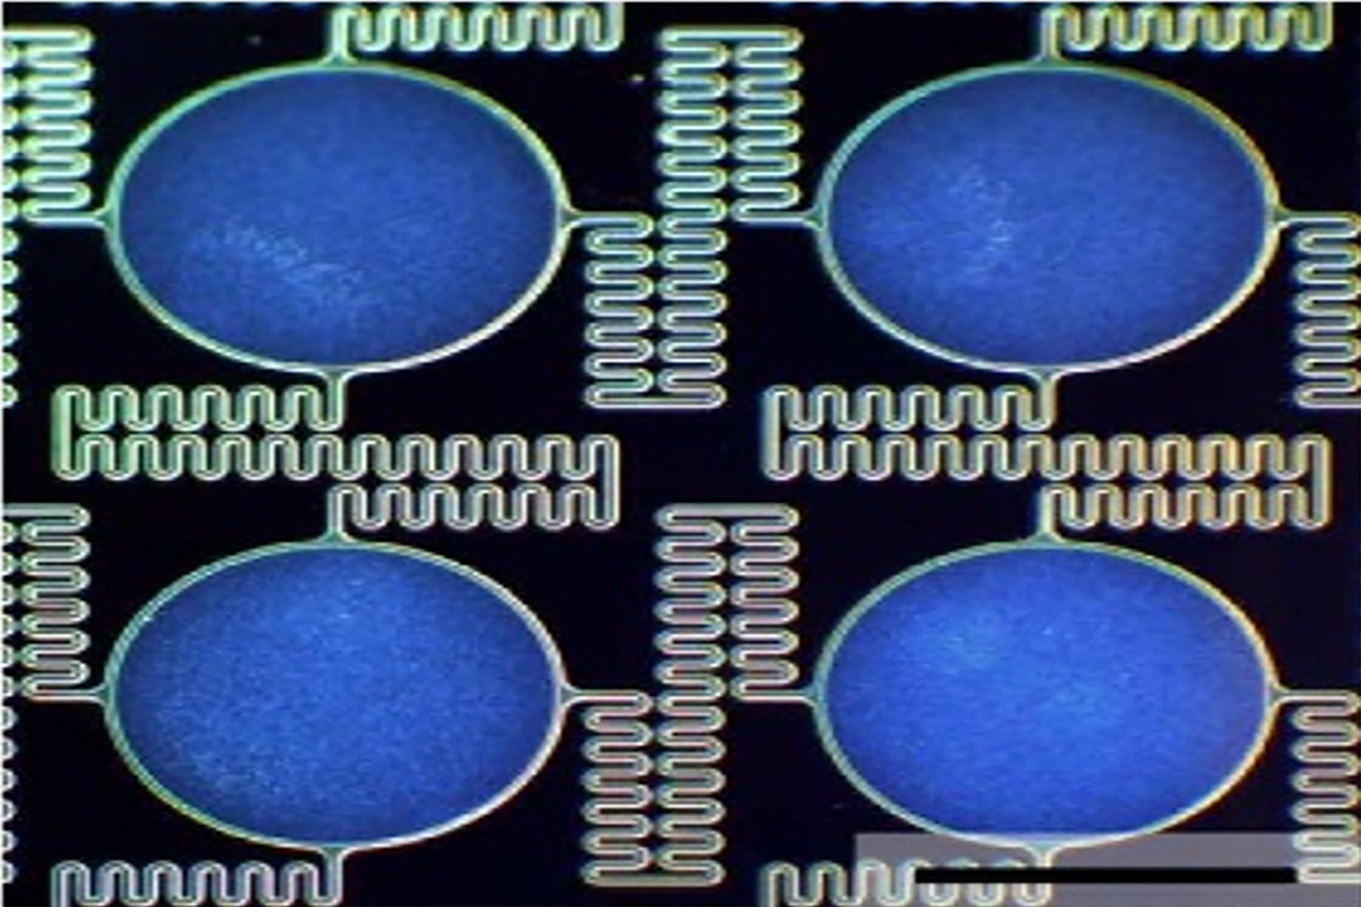
\includegraphics[width=0.45\linewidth]{1_3(2).png}}
	\subcaptionbox{可穿戴发电设备\cite{lai2017single}\label{fig:1_3(4)}}
	{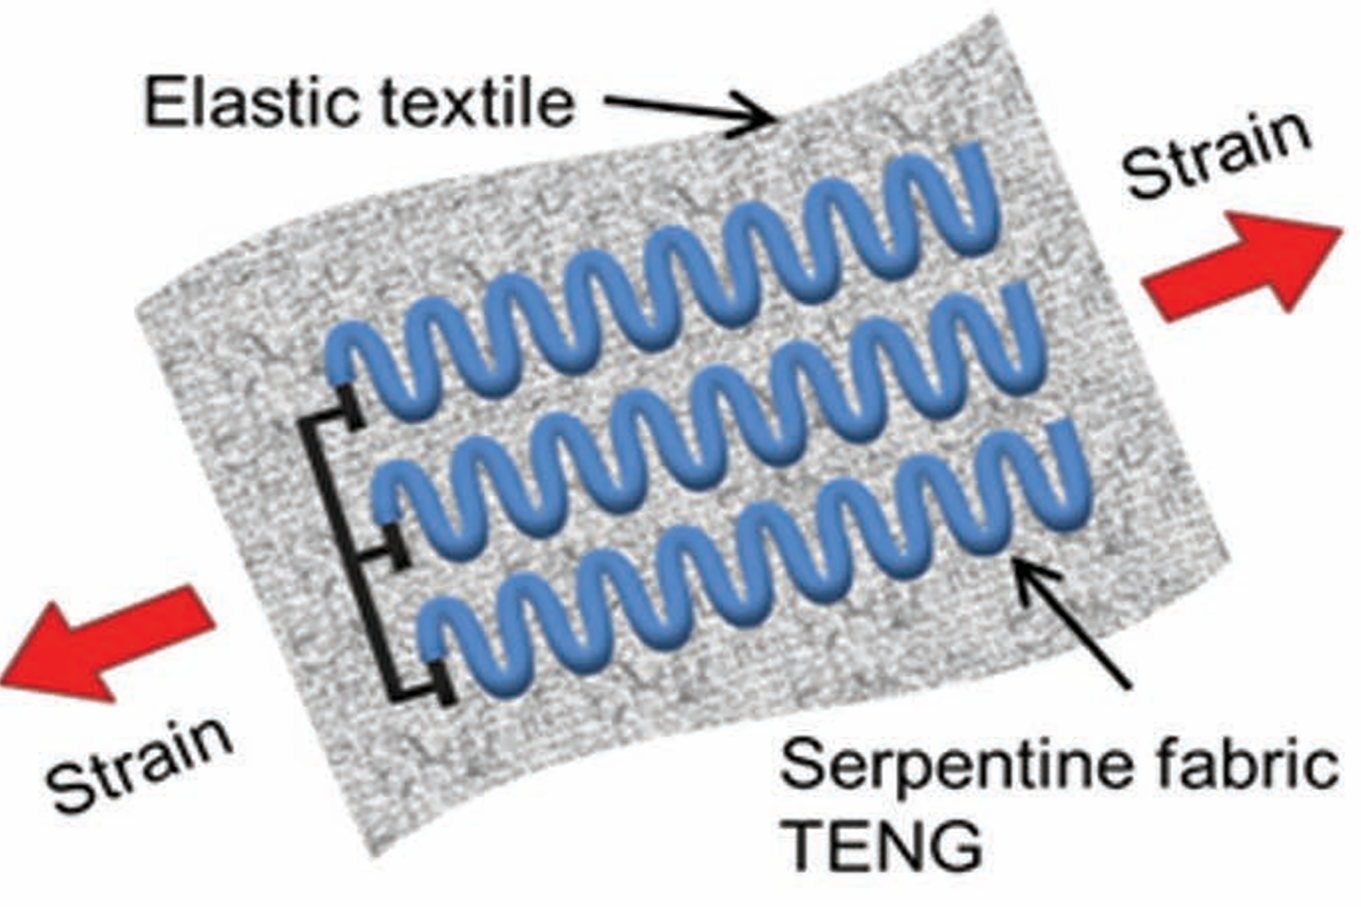
\includegraphics[width=0.45\linewidth]{1_3(1).png}}
	\caption{蛇形结构的实际应用}
	\label{fig:1_3v}
\end{figure}

综上所述,蛇形结构作为一种具有优异可拉伸性能的柔性连接部件,已被广泛应用于可拉伸柔性电子设备中。然而,目前大多数研究主要聚焦于蛇形结构的可拉伸性能,而对其在后屈曲阶段表现出的丰富非线性力学行为(如多稳态行为、稳态间突跳等)尚未充分挖掘和利用。这些非线性行为设计更为智能、自适应的柔性设备提供了潜在的可能性。例如在后屈曲阶段,蛇形结构展现出复杂的力学响应,例如多稳态特性可用于实现结构的自适应变形,而稳态间的突跳行为则可为快速响应提供新的途径。然而,目前对该结构的这些非线性行为的机理研究仍不够深入,缺乏系统的理论分析和实验验证,限制了其在工程实际中的进一步应用。因此,本文将详细研究不同单元数的蛇形结构的后屈曲行为;在此基础上提出优化调控该结构后屈曲行为的方法,为实际的应用提供理论依据,从而推动柔性电子、智能材料等领域的技术进步。


\section{国内外研究现状}
\subsection{弹性蛇形条带结构}
本小节总结了现有文献中关于蛇形条带力学行为的研究成果。基于不同的应用需求,已有研究主要聚焦于以下三个方面:在三维组装技术\cite{cheng2023programming}中,该结构受压屈曲为研究重点;作为振动测量装置时,其振动特性成为研究重点;而在柔性电子设备中,则主要关注其拉伸状态下的力学行为。因此,现有研究主要集中于该结构的受压/受拉屈曲行为及其振动响应特性。

在三维组装技术中\cite{cheng2023programming},蛇形结构常被用作构建目标三维结构的基础平面构型。该技术通过将二维结构(如蛇形条带结构)固定于预拉伸的柔性基底上,当释放基底预拉力时,二维结构将因受压而发生面外屈曲失稳,如图~\ref{fig:1_4(1)}所示。因此,深入研究蛇形结构受压屈曲的力学行为具有重要意义。Li等\cite{li2019mechanics}采用有限元方法,系统研究了蛇形结构的几何参数和材料参数与屈曲构型上最大应变之间的关系。在此基础上,Zhao等\cite{zhao2021torsional}进一步发展了一套力学模型,详细刻画了蛇形结构受压屈曲后的构型特征,包括构形曲率、挠率以及结构中应力分布等关键力学信息。

振动测量方法为表征生物材料的物理特性(如细胞质量和杨氏模量)提供了有效手段,如图~\ref{fig:1_4(2)}所示。蛇形结构受压会失稳屈曲,不同的压力载荷会诱导产生不同的屈曲构型,而每种屈曲构型又具有独特的振动响应特性。因此基于蛇形结构设计的可调谐的振动框架\cite{zhao2021theoretical},能够方便调整配置、振动模式和共振频率。基于此,众多研究聚焦于蛇形结构屈曲后的振动响应特性。例如,Zhao等\cite{zhao2023theoretical}建立了理论模型来预测蛇形结构的振动行为,并推导出了预测结构固有频率的解析表达式。
\begin{figure}
	\centering
	\subcaptionbox{蛇形结构的三维组装\cite{jiao2023vertical}\label{fig:1_4(1)}}
	{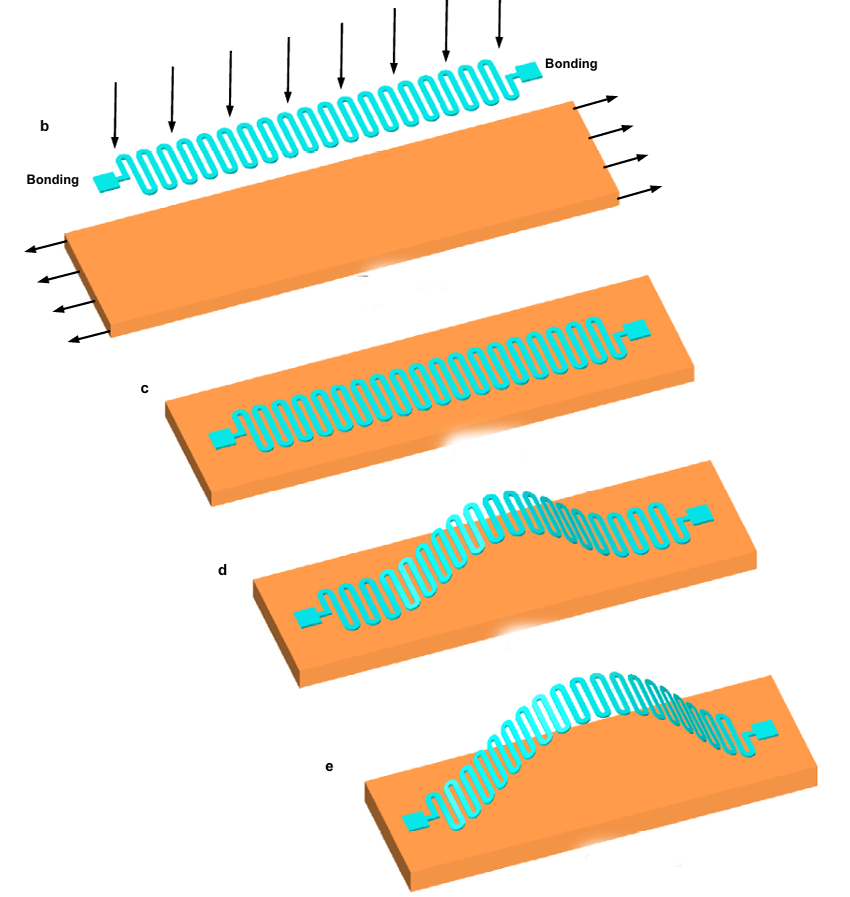
\includegraphics[width=0.45\linewidth]{1_4(1).png}}
	\subcaptionbox{蛇形结构可调谐振动测量装置 \cite{zhao2021theoretical}\label{fig:1_4(2)}}
	{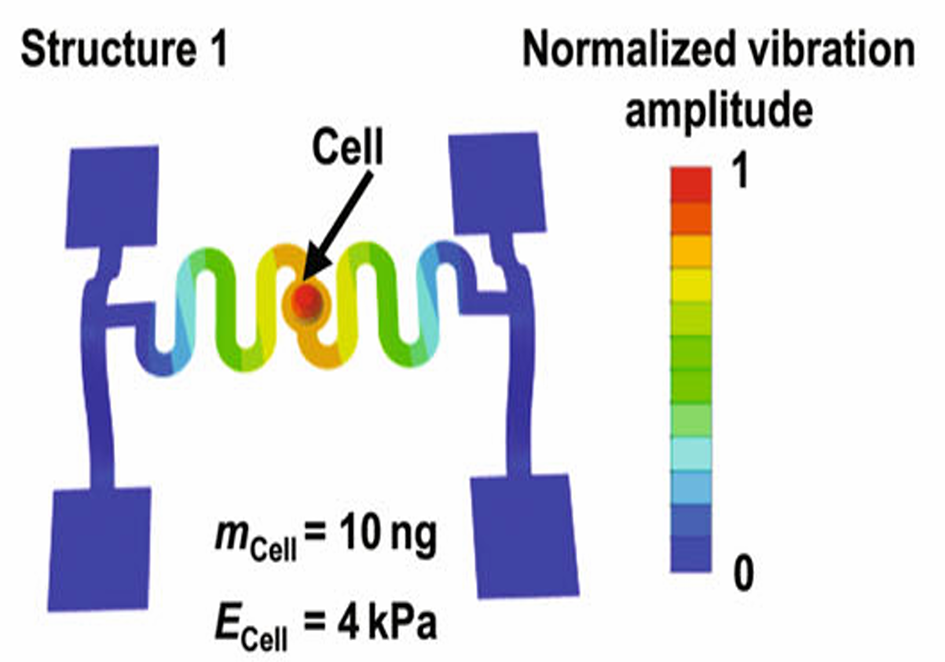
\includegraphics[width=0.45\linewidth]{1_4(2).png}}
	\caption{蛇形结构受压屈曲的应用}
	\label{fig:1_4v}
\end{figure}

对蛇形结构在拉伸载荷下力学行为的研究主要可分为两类:一类聚焦于结构未发生面外失稳时的平面解,另一类则关注结构失稳后的屈曲行为。在对平面解的研究中,Widlund等\cite{widlund2014stretchability}针对宽厚比较小(不易发生失稳)的蛇形结构,基于曲梁理论给出了的解析解,并通过有限元数值模拟验证了解析结果的准确性。Fan等\cite{fan2016finite}基于有限变形理论,提出了非线性的解析表达式,进一步完善了蛇形结构平面解的理论模型。

在对蛇形结构的屈曲行为研究中,Feng等\cite{feng2020analytical}推导了蛇形结构的无量纲临界屈曲载荷与长宽比之间的简单比例关系。Zhang等\cite{zhang2013buckling}通过有限元计算,揭示了单单元蛇形条带在两端固支的边界条件下,蛇形条带存在两类失稳模态分别为反对称稳态(如图~\ref{fig:1_5}中第二行第一列所示)和对称稳态(如图~\ref{fig:1_5}中第二行第一列所示)。随着高宽比的增加,蛇形条带失稳模态由反对称转变为正对称模态。而对于多单元蛇形结构只存在反对称稳态,如图~\ref{fig:1_5}中第一行第一列所示,其屈曲模态与高宽比无关。

通过对蛇形结构研究现状的分析可以发现,在实际应用中该结构往往处于后屈曲状态。因此,深入研究蛇形结构的后屈曲力学行为对于指导工程应用具有重要的理论和实践意义。然而,现有研究主要局限于对一阶屈曲模态的分析,对后屈曲状态下丰富的非线性力学行为的研究仍显不足。具体而言,虽然Zhang等\cite{zhang2013buckling}揭示了屈曲模态与结构高度之间的关联性,但尚未给出相应的力学机理解释。此外,该结构在后屈曲阶段表现出的多稳态特性也缺乏系统研究。基于此,本研究将系统探究蛇形结构在后屈曲阶段的非线性力学行为,重点包括屈曲模态交换机制、多稳态特性及分岔行为等关键问题。


\subsection{细长结构稳定性分析}
蛇形结构具有复杂的分岔行为,在分岔点前后平衡路径的稳定性往往会发生改变,而平衡解的失稳往往对应着结构屈曲以及结构突跳等行为,因此,准确判定平衡分支的稳定性对研究蛇形结构的非线性行为至关重要。细长结构在各种载荷和各类约束下的稳定性问题,是弹性理论最基本且最古老的问题之一,其历史可以追溯到欧拉对弹性杆的研究。目前,关于细长弹性杆稳定性分析的研究大致可分为两类:一类是静力学方法,主要基于能量最小原理进行稳定性判断;另一类则是基于动力学稳定性判断准则的方法。

静力学稳定性判断方法基于能量最小原理,根据势能理论,处于稳定平衡状态的结构其弹性能通常对应于势能函数的局部最小值。能量泛函取得最小值不仅要满足能量泛函一阶变分为零,同时也要保证二阶变分的非负性。通过考虑平衡解对应的雅可比方程\cite{gelfand2000calculus}(二阶常微分方程),若雅可比方程存在非零解,且该解在定义域中不会穿过横坐标(无共轭点),那么根据雅可比强条件,可以说明该平衡解为稳定解。Morse等\cite{morse1951introduction}证明了若在定义域的端点不是共轭点,那么定义区间内共轭点数与平衡解指数相等。因此,稳定性的判定归结为定义区间内是否存在共轭点\cite{gelfand2000calculus}(conjugate point)的判断。

对于边界条件为Dirichlet条件的保守系统而言,共轭点可以用来判断解的稳定性。Manning等\cite{manning1998isoperimetric}将共轭点测试方法用于对DNA结构的稳定性判断。同时,通过对稳定性矩阵行列式的计算,提高了判断解稳定性的计算效率。Hoffman等\cite{hoffman2002calculation}通过共轭点测试对端部受扭转的不可拉伸梁的稳定性进行了判断。提出了一种通过对特定载荷参数下(弧长1处为共轭点的载荷)共轭点测试的方法,来判断结构的稳定性,避免了在载荷参数变化后,判断稳定性需要重新求解微分方程的初值问题所带来的计算成本。

对于Neumann–Neumann边界条件的系统而言,Manning等\cite{manning2009conjugate}将通过共轭点测试判断结构稳定性的方法推广到Neumann–Neumann边界条件的情形。在该文章中讨论了有限维系统的海森矩阵的谱与二阶变分算符的谱的关系。

另一种稳定性判断方法则是基于动力学稳定性准则。Goriely等\cite{goriely2000nonlinear}通过在三维细长结构平衡解附近施加扰动的方法来判断结构在该平衡解的稳定性。通过摄动法,对平衡解加入扰动项,线性化扰动方程,提出了动力学变分方程,用来判断解的稳定性。通过非线性的分析得到了幅值方程,用来描述失稳后的动力学行为。该文章通过非线性Klein-Gordon方程来描述初始曲率为零的细长杆失稳后的运动模式。

Kumar等\cite{kumar2010generalized}根据动力学稳定性判据,对细长结构的动力学方程通过有限元进行离散,离散后对系统稳定性的判断归结为奇异矩阵的广义特征值问题。该文章提出了一种求解奇异矩阵的广义特征值的算法,从而进行稳定性的判断。该方法可以处理更加广泛的边界条件,包括积分约束条件,多点约束条件。

Liu等\cite{liu2011stability}在动力学Cosserat模型下,通过给螺旋线在平衡解处施加扰动的方法研究螺旋线的稳定性,给出了失稳的临界载荷。揭示了Lyapunov稳定性概念和欧拉稳定性概念在细长结构稳定性判断上的区别,Lyapunov稳定性判断为稳定的解,实际上已经发生了屈曲。对于螺旋线而言,在空间域上的Lyapunov和欧拉稳定性条件是在时间域上Lyapunov稳定性条件的必要条件。

由于静力学判定能量泛函极小值的方法对载荷以及边界条件有较大限制,且该方法仅适用于保守系统,对存在非保守力(阻尼力以及跟随力)的系统而言,该方法难以进行稳定性的判定。因此,本文利用动力学系统稳定性概念来对细长结构进行稳定性分析,设计一种算法来对任意曲率的细长结构在任意载荷下的稳定性进行有效判定。
\subsection{结构屈曲行为调控}
结构优化是工程设计中不可或缺的重要环节,其目标是在满足各种约束条件的前提下,寻找最优的结构设计方案。例如,在航空航天领域,往往需要在满足刚度强度等要求下,对结构进行轻量化设计。另外,一些研究者致力于设计多层级结构(同时存在微结构与宏观结构)来实现结构更为良好的特性以及设计多功能材料。为此,目前已发展出包括拓扑优化\cite{jihong2021review}在内的许多结构优化方法来对结构进行优化设计。

蛇形结构被广泛应用于柔性电子设备中,为了满足不同柔性设备的要求,同样需要对该结构进行优化设计。蛇形条带结构良好的可拉伸性是其被广泛应用于柔性电子设备的主要原因,因此一些研究通过优化蛇形结构参数来提高其可拉伸性能,例如,Ye等\cite{ye2022automatic}系统地探讨了蛇形结构的几何参数和材料参数与其最大拉伸应变之间的关系,并提出了相应的优化策略。另外,蛇形条带结构在使用过程中的形变往往会影响结构的导电性能以及信号传输能力\cite{han2022electrical}。其中,Gutruf等\cite{gutruf2014strain}研究了具有不同圆弧段角度的蛇形微电极的电阻应变敏感性。鉴于蛇形结构在承受拉伸载荷时通常处于后屈曲状态,且根据本文实验结果表明该结构在后屈曲阶段表现出显著的非线性行为,因此,通过优化设计手段来调控蛇形结构,以充分利用其非线性特性从而实现更优的性能显得尤为必要。目前,针对该结构的优化研究主要聚焦于其可拉伸性,而对其后屈曲行为的优化尚未得到充分关注。为此,本文将提出一种优化方法,旨在有效调控蛇形结构的后屈曲行为。

过去对结构失稳屈曲行为的优化调控中,主要集中在两个方面,一方面通过优化方法来提高结构的临界失稳载荷,以避免工程结构的失稳,而另一方面,通过优化方法,来调控结构的屈曲构形。在以提高临界失稳载荷为优化目标的优化设计中,往往需要进行特征值分析来决定失稳载荷,例如,Maalawi等\cite{maalawi2002buckling}对具有各种截面形状的柔性杆的截面面积进行优化,给出了多种提高临界失稳载荷的设计方案。Wang等\cite{wang2017buckling}和Wu等\cite{wu2015framework}利用利用优化方法来对网格加筋复合板中的加强纤维的排布方式进行设计,来提高复合板的临界屈曲载荷。不同于以上研究,Lindgaard等\cite{lindgaard2011unified}通过追踪复合材料壳结构的非线性平衡路径,并检测分岔点拐点的出现来得到临界失稳载荷,该方法可以给出更为准确的临界失稳载荷。随后,通过优化这些失稳点的位置以提高临界失稳载荷。

结构在后屈曲阶段展现出的丰富非线性行为可以用来设计多功能结构,因此,一些研究开始聚焦于板壳等薄壁结构在后屈曲阶段的行为并进行优化设计,例如,Li等\cite{li2019harnessing}研究了夹杂对软质多孔结构后屈曲行为以及弹性波在该介质中传播的影响。该研究说明通过改变结构的材料和几何性质,可以有效调控结构的后屈曲模态。Lanzi等\cite{lanzi2006post}通过将有限元与遗传算法(genetic Algorithms)以及全局优化算法来对处于后屈曲范围内的复合材料板进行优化以提高其失效对应的最大载荷。Bochenek等\cite{bochenek2006structural}基于粒子群优化算法来优化结构屈曲后的平衡路径,通过优化结构参数使得结构的平衡路径沿着预定轨迹行进。

本文基于Lindgaard等\cite{lindgaard2011unified}的优化思路,将优化对象由临界失稳载荷对应的分岔点拓展到后屈曲阶段的各类分岔点以实现对后屈曲行为的调控。具体而言,本文中借鉴了对动力系统优化的一种方法:通过优化分岔点的数量及位置来调控动力系统行为\cite{melot:hal-04378993}。本文将该优化策略应用于对蛇形结构后屈曲行为的调控,以实现对蛇形结构的优化设计。
\subsection{研究现状总结}
从上述分析可知,尽管过去对弹性蛇形条带的研究已较为深入地分析了一阶屈曲模态特性,但对其后屈曲状态下表现出的多稳态切换、模态交换等非线性力学行为仍缺乏系统性探索。在蛇形结构的优化方面,现有优化设计主要集中于通过调整几何参数提升结构的可拉伸性,而针对后屈曲行为的主动调控策略尚未建立,这限制了蛇形结构在柔性电子等领域的性能优化。为此,本研究通过实验与数值模拟相结合的方法,系统研究蛇形结构在后屈曲阶段的非线性力学行为,研究成果将为蛇形结构的进一步应用提供了理论基础与设计策略。

\section{主要研究内容与研究方案}
Zhang等\cite{zhang2013buckling}发现单单元蛇形条带的屈曲模态随结构高度的变化而不同,具体而言,当高度小于某一临界高度时,其屈曲构形的二维俯视图表现为反对称形式,如图~\ref{fig:1_5}中第二行第一列所示;而当高度超过该临界值时,屈曲模态则转变为正对称构形,如图~\ref{fig:1_5}中第一行第一列所示,更为清晰的正反对称构形见图~\ref{fig:SM_Mode}。然而,对于多单元蛇形结构,其屈曲构形始终表现为反对称形式,如图~\ref{fig:1_5}中第二三列所示。本文将聚焦于这一现象并揭示该现象背后的机理。此外,基于实验观察,本文发现该结构表现出显著的多稳态特性,因此将进一步对这一多稳态行为展开系统性研究。本文通过数值计算与实验相结合的方法,对该结构进行了详细分析,并对数值结果与实验结果进行了相互验证,以确保研究结论的准确性与可靠性。
\begin{figure}
	\centering
	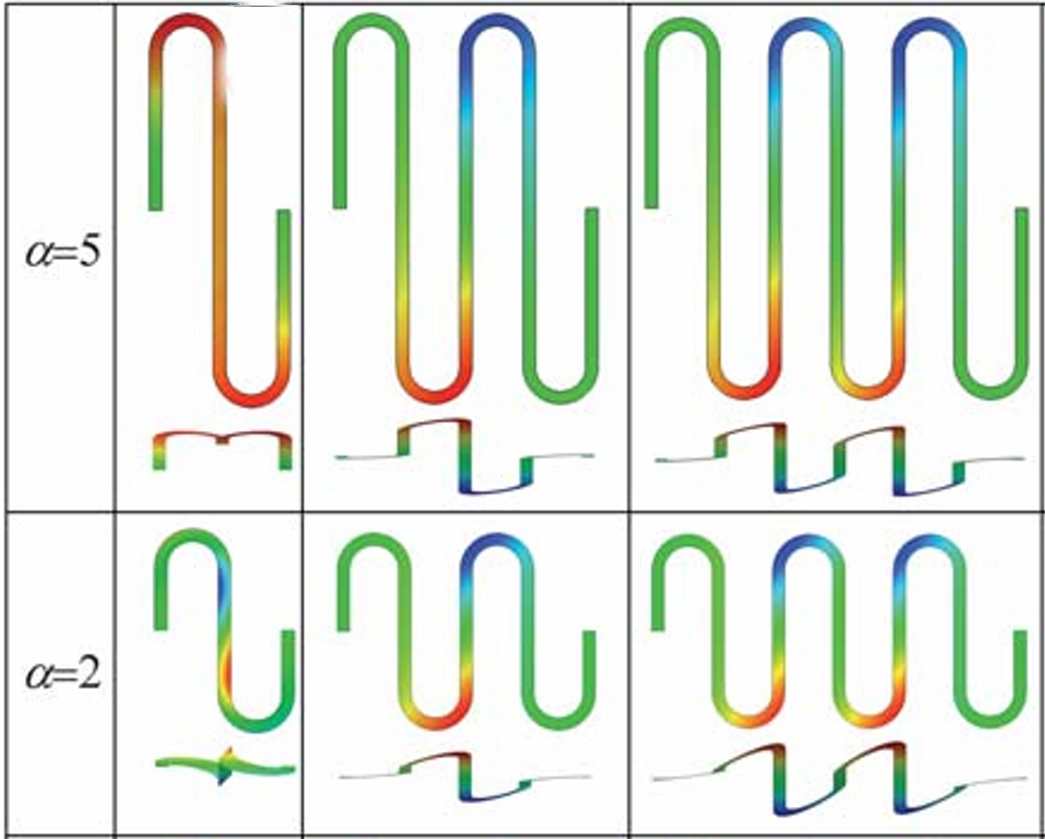
\includegraphics[width=0.6\linewidth]{1_5.png}
	\caption{不同高度,不同单元数的蛇形结构的屈曲模态,图中每一方格内下方图为屈曲模态的二维俯视图\cite{zhang2013buckling}}
	\label{fig:1_5}
\end{figure}

本文首先选取了合理的力学模型对蛇形结构进行建模。具体而言,本文采用了静力学基尔霍夫弹性杆模型\cite{dill1992kirchhoff},该模型忽略了条带结构的拉伸应变能,将条带结构简化为不可拉伸杆。已有研究表明,这种不可拉伸杆模型能够精确捕捉细长条带结构(包括由条带构成的网状结构)的非线性行为\cite{yu2019bifurcations,yu2021numerical}。因此本文将用基尔霍夫杆模型对蛇形结构进行建模,所建立的数学模型为适定的边界值问题。

为了求解此边界值问题并研究该结构的后屈曲行为,本文采用参数延拓法来跟踪平衡路径并判断分岔点的出现\cite{yu2019bifurcations,ahsan2022methods},利用MatLab分岔分析工具包COCO\cite{dankowicz2013recipes}以及分岔分析软件ATUO 07P\cite{doedel2007auto}来求解此边界值问题,并以水平拉伸位移载荷作为延拓参数,跟踪不同载荷下的平衡路径并进行分岔分析。

通过上述的分岔分析可以获得平衡路径,但在无法得到平衡分支上解的稳定性信息。平衡解的失稳往往诱发结构屈曲或平衡态突跳等非线性现象,发展一套有效的细长结构稳定性分析数值方法对蛇形条带力学行为的研究具有关键意义。本文基于动力学稳定性准则进行解的稳定性判定,为此需建立蛇形条带的动力学控制方程。这里采用离散弹性杆(Discrete Elastic Rod,简称DER)动力学模型\cite{jawed2018primer}建立初值形式的动力学方程。通过求解其不动点并计算相应雅可比矩阵来实现稳定性分析。需要特别说明的是,尽管离散弹性杆模型同样也可以对结构进行静力学分析,但离散弹性杆模型中包含了杆的拉伸应变。对于长细比极大的蛇形条带而言,拉伸应变可以忽略不计,需满足不可拉伸条件。为此,利用离散弹性杆模型对条带结构的建模过程中将拉伸刚度视为罚因子,拉伸能项视为罚函数。然而数值结果表明,过大的拉伸刚度将导致病态刚度矩阵的出现,引发数值奇异;而适度罚因子虽能保证计算稳定性,却会引入较小的误差,影响解的精度。为克服这一矛盾,本文提出混合建模策略:采用基尔霍夫杆理论进行平衡分支求解,该模型严格满足不可拉伸假设且能准确描述几何非线性效应;同时利用DER模型进行稳定性分析。

在对蛇形结构多稳态特性的研究方面,本文采用动力学离散弹性杆模型进行动力学模拟,以捕捉结构从一种稳态构形向另一种稳态构形的突跳行为。具体而言,当结构在拉伸载荷下处于某一平衡构形时,通过在该构形上施加适当的扰动力,该结构将从这一平衡构形突跳到其他平衡构形,随后在阻尼的作用下,蛇形结构会逐渐稳定到新的构形上。

蛇形条带结构几何参数的优化设计以及对其屈曲模态的调控在实际应用中具有关键意义。因此,本文在详细研究蛇形条带结构后屈曲行为的基础上,提出一种调控蛇形结构后屈曲行为的方法。该方法通过优化蛇形结构的几何参数,实现对分岔点位置及屈曲模态的主动调控,从而为结构的精确设计提供理论依据。具体而言,在保持结构对称性的条件下,将蛇形结构不同分段的条带厚度以及高度作为优化参数,使用优化工具包NLOPT\cite{NLopt}优化分岔点位置,从而实现结构后屈曲行为的调控。对于单单元蛇形条带,优化目标为调控正对称模态与反对称模态之间的临界高度。对于双单元蛇形条带,优化目标为实现一阶屈曲模态与二阶屈曲模态顺序的交换,进一步验证单单元蛇形结构与双单元蛇形结构中模态交换现象具有相同的数学机理。此外,通过调节蛇形结构的单元厚度,本文进一步揭示了单元厚度的变化能够有效影响结构的屈曲构形,这一发现为屈曲构形的精细化调控提供了新的设计维度。

综上所述,本文中所要研究的问题可阐述如下:
\begin{enumerate}
	\item 正如原始研究\cite{zhang2013buckling}中观察到的情况(一阶屈曲模态随高度增大先后为反对称、正对称),是什么导致了蛇形条带屈曲模态的交换?
	\item 在后屈曲阶段,如何通过数值计算的手段来识别其多个稳定的屈曲构形?
	\item 如何通过几何形状来调控屈曲模式以及临界屈曲载荷?
\end{enumerate}

为了解决上述问题,本文所采用的研究方法主要为:
\begin{enumerate}
    \item 基于动力学稳定性判据来判定条带结构的平衡解的稳定性。
	\item 采用基尔霍夫杆模型对蛇形结构进行建模,并利用分岔分析工具包COCO以及AUTO 07P进行分岔分析。
	\item 采用动力学模拟来研究蛇形结构的多稳态行为。
	\item 通过优化蛇形结构的几何参数,实现对分岔点位置及后屈曲行为的主动调控。
\end{enumerate}


% !TeX root = ../sustechthesis-example.tex

\chapter{弹性杆模型及细长结构稳定性分析}

\section{引言}

建立弹性蛇形条带结构的力学模型是研究其分岔行为和进行结构稳定性分析的基础。由于其细长的几何特性,蛇形条带的弯曲和扭转刚度较低,在外载荷作用下,在满足小应变假设(即线弹性本构关系)的前提下,结构仍会产生较大的位移变形。因此,本文采用基于线性本构关系的弹性杆模型,并考虑结构的几何非线性效应。具体而言,本文主要采用两种弹性杆模型:离散弹性杆模型和基尔霍夫杆弹性杆模型。

离散弹性杆模型中考虑了惯性力,属于动力学模型。因此利用该模型,不仅可以求得结构在给定载荷作用下的平衡解,而且可以利用线性化的动力学稳定性判据来判断平衡解的稳定性;而基尔霍夫杆模型是经典的静力学弹性杆模型,由于该模型为不可拉伸杆模型,更加符合细长杆的建模,因而能给出更为精确的解,但该模型无法直接对所得解的稳定性进行判定。因此,本文结合了两套模型的优势:利用基尔霍夫杆模型进行分岔分析以获得更精确的解,同时利用离散弹性杆模型通过动力学稳定性判定方法对所得解的稳定性进行判断。另外,在后续研究蛇形结构多稳态行为时,仍需要利用动力学模态来寻找稳态解。

本章首先系统介绍离散弹性杆模型与基尔霍夫杆模型的理论框架。随后,详细阐述本文用于分析结构后屈曲行为的主要方法与工具——参数延拓法,以及用于结构稳定性判定的理论依据。最后,通过对典型结构的计算分析,验证基于线性化的动力学稳定性判据在判定平衡解稳定性方面的有效性。

\section{基尔霍夫杆模型}
\subsection{标架运动学方程}
根据微分几何的曲线论基本定理可知,任意一条空间曲线的构形可以由该曲线在任意弧长处的曲率和挠率两个量完全确定。在刻画一条空间曲线的构形时,通常会在任意弧长处定义一个Frenet标架,该标架的第三个坐标轴与曲线相切;第一个坐标轴指向曲线的弯曲方向,即与$d\overrightarrow{\mathbfit{t}}/\dif s$共线,其中$\overrightarrow{\mathbfit{t}}$为曲线的单位切向量,称为主法向量;第二个坐标轴与其他两个坐标轴共同构成构成右手坐标系,称为次法向量。

而为了确定一根细长弹性杆的空间构形,不仅仅需要确定中心线的空间位置,还需确定任意弧长处弹性杆截面的空间取向。细长弹性杆的几何构形通常可以用一条框架曲线来刻画,如图~\ref{fig:Material Frame}所示。红色虚线为弹性杆的中心线,并且在该曲线的任意弧长处附有一材料标架用来刻画细长弹性杆截面的空间方位。该标架的原点在中心线上,三个坐标轴分别与曲线的切线$\mathbfit{t}$以及弹性杆截面的两个主惯性轴$\mathbfit{d}_1,\mathbfit{d}_2$共线。因此,一根弹性杆可以由三个量来确定:任意弧长处的曲率,挠率,以及材料标架与Frenet标架绕共同切线轴的相对转角。
\begin{figure}
	\centering
	\includegraphics[width=0.8\linewidth]{Material frame.pdf}
	\caption{细长杆变形前后相应的框架曲线}
	\label{fig:Material Frame}
\end{figure}

下面给出材料标架的沿弧长的运动学关系,由于材料标架三个轴总保持互相垂直,因此材料标架对弧长$s$的导数满足
    \begin{equation}
    \centering
	\mathbfit{d}'_{\alpha}=\mathbfit{\Omega}\times\mathbfit{d}_{\alpha},\quad
	\mathbfit{\Omega}=\mathbfit{t}\times \mathbfit{t}'+m \mathbfit{t}   
    \label{eq:Darboux vector}
    \end{equation}
式中下标$\alpha$可以取$1$,$2$,$3$分别对应材料标架的三个坐标轴,这里$\mathbfit{d}_3$轴为$\mathbfit{t}$轴。$\mathbfit{\Omega}$称为Darboux向量,该向量用来刻画材料标架沿弧长的变化率,可以分两部分:第一部分为$\kappa \mathbfit{b}=\mathbfit{t}\times \mathbfit{t}'$,该项保证了材料标架沿弧长变化过程中坐标轴$\mathbfit{t}$总是与中心线相切;第二部分中$m=\mathbfit{d}'_1 \cdot \mathbfit{d}'_2$,该项用来刻画材料标架沿弧长绕切线轴转动的变化率。

在实际计算过程中,为了避免由于欧拉角的引入而产生可能的数值奇异,本文采用四元数来刻画材料标架随弧长的转动,设Darboux向量$\mathbfit{\Omega}=\kappa_1\mathbfit{d}_1+\kappa_2\mathbfit{d}_2+\tau \mathbfit{t}$,四元数为$\mathbfit{q}=(q_1,q_2,q_3,q_4)$,Darboux向量与四元数导数的关系如式\eqref{eq:Derivative of Quaternion}所示
\begin{equation}
	\centering 
	\begin{split}
    &q_1'=\frac{1}{2}(-\kappa_1 q_2-\kappa_2 q_3-\tau q_4) \\
    &q_2'=\frac{1}{2}(\kappa_1 q_1+\tau q_3-\kappa_2 q_4) \\
    &q_3'=\frac{1}{2}(\kappa_2 q_1-\tau q_2+\kappa_1 q_4) \\
    &q_4'=\frac{1}{2}(\tau q_1+\kappa_2 q_2-\kappa_1 q_3) \\
\end{split}
	\label{eq:Derivative of Quaternion}
\end{equation}


\subsection{平衡方程及本构关系}
本小节将通过微元法来推导细长弹性杆的平衡方程并给出本构关系。
\begin{figure}
	\centering
	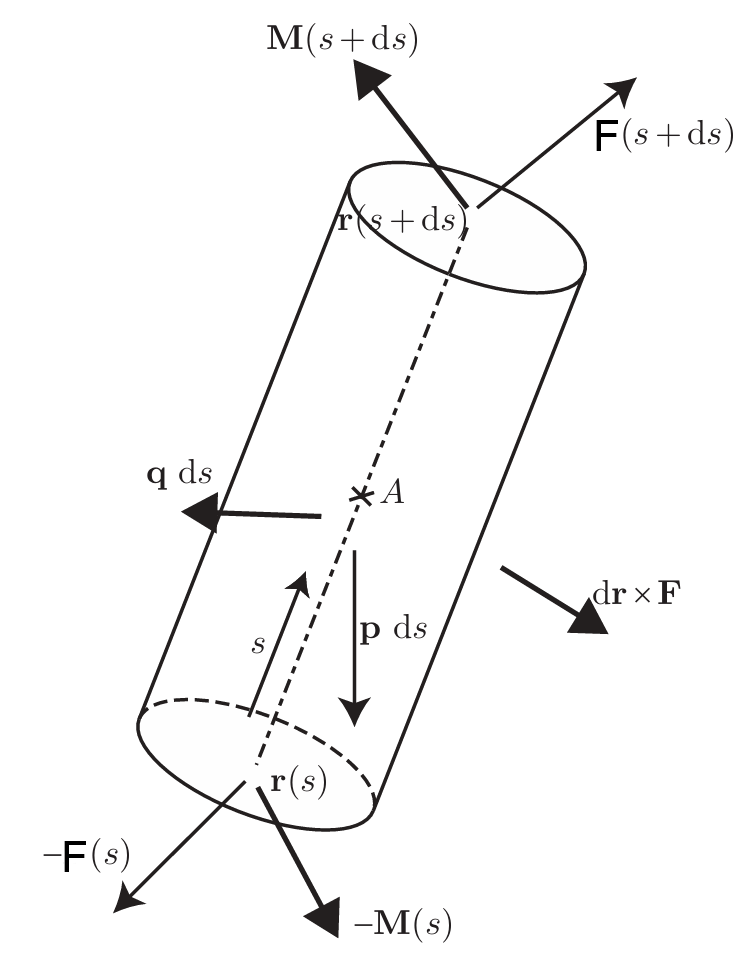
\includegraphics[width=0.5\linewidth]{equilibrium equation.pdf}
	\caption{弹性杆微元的受力图,$\mathbfit{F}$,$\mathbfit{M}$为截面上所受力与力矩,$\mathbfit{p}$,$\mathbfit{q}$为微元上分布力与分布力矩\cite{audoly2000elasticity}}
	\label{fig:Equilibrium equation}
\end{figure}
图~\ref{fig:Equilibrium equation}为弹性杆微元的受力分图,根据受力图,易得力平衡方程及力矩平衡方程,分别为
\begin{equation}
	\centering
	\begin{gathered}
		\mathbfit{F}(s+\dif s)-\mathbfit{F}(s)+\mathbfit{p}\dif s=0 \\
		\mathbfit{M}(s+\dif s)-\mathbfit{M}(s)
		+(\mathbfit{d}\mathbfit{r}/2)\times\mathbfit{F}(s+\mathbfit{d}s)
		-\mathbfit{dr}/2\times(-\mathbfit{F}(s))
		+\mathbfit{q}\dif s=0	
	\end{gathered}   
	\label{eq:Equilibrium equation}
\end{equation}
式中,$\mathbfit{F}$为作用在截面上的内力,$\mathbfit{p}$为作用在微元上的分布力,$\mathbfit{M}$为作用在截面上的内力矩,$\mathbfit{q}$为分布力矩。其中力矩平衡方程是关于点$A$的力矩平衡方程。将式\eqref{eq:Equilibrium equation}两端同时除以微元长度$\dif s$并忽略高阶项得
\begin{equation}
	\begin{split}
		&\mathbfit{F}'(s)+\mathbfit{p}(s)=0 \\
		&\mathbfit{M}'(s)
		+\mathbfit{d}_3(s)\times\mathbfit{F}(s)
		+\mathbfit{q}(s)=0	
	\end{split}   
	\label{eq:Equilibrium equation1}
\end{equation}

下面将介绍基尔霍夫杆的本构关系。该本构关系仅在小应变假设成立的条件下适用,即细长杆变形后曲率半径$R$远远大于细长杆截面的特征长度$h$的情况($R>>h$)下适用,本文所研究的结构该假设总成立。基尔霍夫杆的本构关系为线性关系,设Darboux向量为$\mathbfit{\Omega}=\kappa_1\mathbfit{d}_1+\kappa_2\mathbfit{d}_2+\tau \mathbfit{t}$,则该本构关系的具体表达式为式如\eqref{eq:Constitutive Law}所示
\begin{equation}
	\begin{split}
		&\mathbfit{M}(s)=G^{(1)}(s)\mathbfit{d}_1(s)+G^{(2)}(s)\mathbfit{d}_2(s)+H(s)\mathbfit{t}(s) \\
		 &G^{(1)}(s)=EI^{(1)}(\kappa_1(s)-\kappa_{10}(s))\\ 
		&G^{(2)}(s)=EI^{(2)}(\kappa_2(s)-\kappa_{20}(s))\\
		 &H(s)=G J\tau(s)	
	\end{split}   
	\label{eq:Constitutive Law}
\end{equation}
式中,$\kappa_{10}(s)$,$\kappa_{20}(s)$为弹性杆的初始曲率,$EI^{(1)}$,$EI^{(2)}$分别为绕主惯性轴$d_1$,$d_2$的弯曲刚度,$G J$为弹性杆的扭转刚度。
其中$E$为弹性模量,$G$为剪切弹性模量$G=E/2(1+\nu)$,$J$为极惯性矩,$\nu$为泊松比,本文中泊松比设为$0.33$。本文所研究的结构均为具有矩形截面形状的条带结构,这里给出矩形截面的条带结构的弯曲刚度与扭转刚度的具体表达式~\cite{timoshenko1969theory}:
\begin{equation}
	\begin{gathered}
  EI=\frac{1}{12}Ewt^3,\quad EI=\frac{1}{12}Ew^3t,\quad G J=\lambda w\frac{E}{2(1+\nu)}t^3 \\
  \lambda=\frac{1}{3}\left(1-\frac{192}{\pi^5}\frac{t}{w}\sum_{k=1}^{\infty}\frac{1}{(2k-1)^5}\tanh\left(\frac{\pi(2k-1)w}{2t}\right)\right)
  \end{gathered}
\end{equation}
式中,$w$,$t$分别为弹性杆截面的宽度和厚度。另外,拉伸刚度为$Ewt$,其量级为$o(h^2)$,$h$为截面特征长度。而弯曲刚度与扭转刚度的量级为为$o(h^4)$。由于特征长度$h$为小量,弹性杆的拉伸刚度远大于弯曲扭转刚度,因此基尔霍夫杆模型中,忽略拉伸引起的应变及相应的应变能,即基尔霍夫杆为不可拉伸杆。

在实际的计算过程中,需要将矢量方程表达为标量分量形式。由于上述给出的本构关系表达式是在局部材料标架下的投影形式,因此,为了方便本构关系的表达,这里选择将平衡方程同样在局部材料坐标系下投影,力的平衡关系式如下:
\begin{equation}
	\begin{split}
	&N_{1}^{\prime}=N_{2} \tau-N_{3} \kappa_{2}\\
	&N_{2}^{\prime}=-N_{1} \tau+N_{3} \kappa_{1}\\
	&N_{3}^{\prime}=-N_{2} \kappa_{1}+N_{1} \kappa_{2}
	\end{split}
\end{equation}
式中 $N_1$,$N_2$,$N_3$分别为弹性杆截面内力$\mathbfit{F}$在材料标架$\mathbfit{d_1}$,$\mathbfit{d_2}$,$\mathbfit{t}$下的分量。力矩平衡方程的分量表达式为
\begin{equation}
	\begin{split}
	&\frac{\mathrm{d} G^{(1)}}{\mathrm{d} s}-G^{(2)} \tau+H \kappa^{(2)}-N_{2}+q_{1}=0 \\
	&\frac{\mathrm{d} G^{(2)}}{\mathrm{d} s}-H \kappa^{(1)}+G^{(1)} \tau+N_{1}+q_{2}=0 \\
	&\frac{\mathrm{d} H}{\mathrm{d} s}-G^{(1)} \kappa^{(2)}+G^{(2)} \kappa^{(1)}+q_{3}=0
	\end{split}
\end{equation}
式中$q_{1}$,$q_{2}$,$q_{3}$分别为分布力矩在材料标架$\mathbfit{d_1}$,$\mathbfit{d_2}$,$\mathbfit{t}$下的分量。本处需要强调,在表达力与力矩的分量时,由于材料标架不是固定标架而是沿弧长变化的标架,因此在求导数时,应当考虑标架本身的导数,即	$\mathbfit{d}'_{\alpha}=\mathbfit{\Omega}\times\mathbfit{d}_{\alpha}$。
\subsection{边界值问题的构造}
为了求解给定细长结构在外载荷下的非线性行为,需要将该力学问题构造为一个适定的边界值问题。前几小节中,给出了细长弹性杆力与力矩的平衡方程,材料标架的运动方程。此外,为了得到弹性杆中心线的位置,需要通过对切向量沿弧长进行积分,若规定材料标架的切向量对应于全局坐标系的$Z$轴$(0,0,1)$,中心线位置与切向量的微分关系为
\begin{equation}
	\begin{split}
	&x^{\prime}=2\left(q_{2} q_{4}+q_{1} q_{3}\right)\\ 
	&y^{\prime}=2\left(q_{3} q_{4}-q_{1} q_{2}\right)\\ 
	&z^{\prime}=2\left(q_{1}^{2}+q_{4}^{2}-\frac{1}{2}\right)
	\end{split}
\end{equation}
若切向量不与全局坐标系的$Z$轴对应,可通过关系式\eqref{eq:the different compoments in different frames}得到中心线的位置。
\begin{equation}
	\mathbfit{t}=\mathbfit{R}_q(\mathbfit{q})^{\top}\mathbfit{t}^{(1)}
	\label{eq:the different compoments in different frames}
\end{equation}
式中$\mathbfit{t}$,$\mathbfit{t}^{(1)}$分别为曲线切向量在全局坐标系和材料标架下的分量,$\mathbfit{R}_q(\mathbfit{q})$为以四元数表示的全局坐标系与材料标架之间的旋转矩阵\cite{henderson1977euler},具体如下:
\begin{equation}
	\mathbfit{R}_{q}(\mathbfit{q})= 2\left[\begin{array}{ccc}q_{1}^{2}+q_{2}^{2}-\frac{1}{2} &  q_{2} q_{3}+ q_{1} q_{4} &  q_{2} q_{4}- q_{1} q_{3} \\ q_{2} q_{3}- q_{1} q_{4} & q_{1}^{2}+q_{3}^{2}-\frac{1}{2} &  q_{3} q_{4}+ q_{1} q_{2} \\ q_{2} q_{4}+ q_{1} q_{3} &  q_{3} q_{4}- q_{1} q_{2} & q_{1}^{2}+q_{4}^{2}-\frac{1}{2}\end{array}\right] 
		\label{eq:Rotation Matrix}
\end{equation}

在实际计算中,将弹性杆长度进行归一化处理,若弹性杆长度为$l$,$s\in(0,l)$,为了进行归一化处理,这里将方程中变量替换为$s$替换为$\overline sl$,$\overline s\in(0,1)$。在变量替换过程中为了保持原方程不变,对于导数项则需要利用链式法则进行求导,首先对$\overline s$求导,随后将$\overline s$对$s$求导得$1/l$。以变量$\mathrm{d}N_1(s)/\mathrm{d}s$为例,变量替换后该项应为$\mathrm{d}N_1(\overline s)/\mathrm{d}\overline{s}/l$。

综上所示,为了求解计算细长弹性杆的分岔行为,前几小结给出了13个方程,分别为三个力平衡方程,三个力矩平衡方程(带入本构关系,用Darboux向量来表示该平衡方程),四个由四元数表示的材料标架的运动方程,以及三个表示中心线位置与切向量关系的方程。设一弹性杆的长度为$l$,截面形状为矩形,那么相应的微分方程总结如下,
\begin{equation}
	\begin{split}
	&N_{1}^{\prime}=(N_{2} \tau-N_{3} \kappa_{2})l\\
	&N_{2}^{\prime}=(-N_{1} \tau+N_{3} \kappa_{1})l \\
	&N_{3}^{\prime}=(-N_{2} \kappa_{1}+N_{1} \kappa_{2})l \\
	&a \kappa_{1}^{\prime}=(b\left(\kappa_{2}-\kappa_{20}\right) \tau-\tau \kappa_{2}+N_{2})l \\
	&b \kappa_{2}^{\prime}=(-a (\kappa_{1}-\kappa_{10}) \tau+\tau \kappa_{1}-N_{1})l \\\
	&\tau^{\prime}=(-b\left(\kappa_{2}-\kappa_{20}\right) \kappa_{1}+a (\kappa_{1}-\kappa_{10}) \kappa_{2})l \\ 
	&q_{1}^{\prime}=\frac{1}{2}\left(-q_{2} \kappa_{1}-q_{3} \kappa_{2}-q_{4} \tau\right)l+\mu q_{1}l\\
	&q_{2}^{\prime}=\frac{1}{2}\left(q_{1} \kappa_{1}-q_{4} \kappa_{2}+q_{3} \tau\right)l+\mu q_{2}l\\ 
	&q_{3}^{\prime}=\frac{1}{2}\left(q_{4} \kappa_{1}+q_{1} \kappa_{2}-q_{2} \tau\right)l+\mu q_{3}l\\ 
	&q_{4}^{\prime}=\frac{1}{2}\left(-q_{3} \kappa_{1}+q_{2} \kappa_{2}+q_{1} \tau\right)l+\mu q_{4}l \\
	&x^{\prime}=2\left(q_{2} q_{4}+q_{1} q_{3}\right)l\\
	&y^{\prime}=2\left(q_{3} q_{4}-q_{1} q_{2}\right))l\\
	&z^{\prime}=2\left(q_{1}^{2}+q_{4}^{2}-\frac{1}{2}\right)l\\
    &\mu^{\prime}=0
	\end{split}
	\label{eq:ToTle Equation}
\end{equation}
式中, $a$,$b$分别为无量纲化后的两个主惯性轴方向的弯曲刚度。将细长弹性杆的扭转刚度设为1,作为单位来对弯曲刚度进行无量纲化。具体表达式如下
\begin{equation}
	a=\frac{E I_{1}}{G J}=\frac{(1+v)}{6 \lambda}, b=\frac{E I_{2}}{G J}=\frac{(1+v)}{6 \lambda}\left(\frac{w}{t}\right)^{2}
\end{equation}

为了求解细长弹性杆的非线性行为,除了给定结构的控制方程外,还有需要给定相应的边界条件。本文所讨论的主要结构为蛇形条带,其边界条件为两端固支边界条件。由初始端($s=0$)固支条件可以给出七个边界条件,即初始端的位置向量以及由四元数给出的初始端截面空间取向。同理,在末端处($s=1$)可以施加同样的七个边界条件,总共构成$14$个边界条件,而方程个数为$13$。这种方程个数与边界条件个数不匹配的原因是由于四元数四个分量之间并非相互独立,存在下述约束关系式
\begin{equation}
	{q_1}^2+{q_2}^2+{q_3}^2+{q_4}^2=1
	\label{eq:constraint term}
\end{equation}

为了解决方程个数与边界条件个数不匹配的问题,本文采用Healey~\cite{healey2005straightforward}所提出的方法,通过引入常变量$\mu$来解决方程适定性的问题。对于变量之间存在代数约束的微分方程
\begin{equation}
	\begin{split}
	&\dot{\mathbfit{x}}=\mathbfit{f}(\mathbfit{x})\\
	&E(\mathbfit{x})\equiv C
	\end{split}
	\end{equation}
可以通过引入常变量$\mu$来构造一个增广系统
\begin{equation}
		\dot{\mathbfit{x}}=\mathbfit{f}(\mathbfit{x})+\mu \nabla E(\mathbfit{x}), \quad a<t<b
\end{equation}
若方程的一个解满足关系(可由边界条件保证)
\begin{equation}
	E(\mathbfit{x}(a))=E(\mathbfit{x}(b))
\end{equation}
那么该增广系统的解与原方程解一致,且代数约束自动满足。

因此,本文中在四元数表示的材料标架运动方程中增加约束关系\eqref{eq:constraint term}的微分项$2\mu \mathbfit{q}$,即\eqref{eq:ToTle Equation}中的第七到第十个方程的左端第二项。另外,增加方程的常变量$\mu'=0$的关系,即\eqref{eq:ToTle Equation}中的第十四个等式。通过引入常变量原方程由13个增加到14个,使得边界条件个数与方程个数一致。

\section{离散弹性杆模型}
\subsection{控制方程}
离散弹性杆模型(Discrete Elastic Rod)是基尔霍夫弹性杆的一种离散形式。该模型考虑结构所受的惯性力,是细长弹性杆的动力学模型,该模型将一个具有任意自然曲率的细长弹性杆沿弧长进行离散,离散为有限自由度的质点系统,如图~\ref{fig:DER_Schematic}所示。另外,为了刻画弹性杆的扭转程度,在每一离散段上还定义有一个角度,具体的定义过程将在下一小节讨论。因此,若一个弹性杆被离散为$N$段,那么离散系统的自由度为$3(N+1)+N=4N+3$。下文中与节点有关的物理量将用下标来表示对应的节点序号,与离散段有关的量用上标来表示其所属的离散段。
\begin{figure}
	\centering
	\includegraphics[width=0.8\linewidth]{DER_Schematic.pdf}
	\caption{离散弹性杆示意图。$\mathbfit{e}$为连接两两节点的向量,方向指向弧长增大的方向;$\mathbfit{x}$表示节点坐标}
	\label{fig:DER_Schematic}
\end{figure}

为了得到离散弹性杆的动力学控制方程,需要从两个方面入手。首先,需要定义结构的惯性项,为此,需要得到节点的质量和离散段绕其中心轴的转动惯量,其中某一节点处的质量定义为相邻两离散段的质量之和的一半。有了质量的定义与转动惯量的定义,通过质量乘以节点速度,转动惯量乘以扭转角变化率可以得到相应的动量及角动量。另一方面要正确定义其弹性势能,一旦给定弹性势能的表达式,可以通过对能量求导得到广义力。通过以定义的动量和角动量,广义力以及相应的外力,可以列出相应的控制方程。

为了给出离散弹性杆的弹性势能,先考虑连续弹性杆的弹性势能,然后通过离散连续杆的弹性势能来得到离散弹性杆对应的弹性势能。对于连续弹性杆而言,其弹性势能由三部分组成:拉伸弹性能,弯曲和扭转弹性能,具体表达式为
\begin{equation}
	\mathrm{E}_{\mathrm{rod}}=\int \mathrm{d} s\left(EA\varepsilon^2+\frac{E I^{(1)}}{2}\left(\kappa^{(1)}(s)\right)^{2}+\frac{E I^{(2)}}{2}\left(\kappa^{(2)}(s)\right)^{2}+\frac{G J}{2}(\tau(s))^{2}\right)
\end{equation}
式中$EA$,$EI^{(1)}$,$EI^{(2)}$,$G J$分别为拉伸刚度,两个主惯性轴方向的弯曲刚度及扭转刚度。$E_\mathrm{rod}$ 为总弹性势能。在离散弹性杆模型中,将该弹性能进行离散处理,即将弹性能的积分符号离散为求和号,具体表达式如下
\begin{equation}
	\begin{split}
	&E_{s}=\frac{1}{2} \sum_{i=0}^{n-1} E A^{i}\left(\frac{\left\|\mathbfit{e}^{i}\right\|}{\left\|\overline{\mathbfit{e}}^{i}\right\|}-1\right)^{2}\left\|\overline{\mathbfit{e}}^{i}\right\| \\
	&E_{t}=\frac{1}{2} \sum_{i=1}^{n-1} G J_{i} \left(\frac{m_{i}-\overline{m}_{i}}{\overline{\ell}_{i}}\right)^{2}{\overline{\ell}_{i}} \\
	&E_{b}=\frac{1}{2} \sum_{i=1}^{n-1} 
	E I^{(1)}\left(\frac{\kappa_{i_{1}}-\overline{\kappa}_{i_{1}}}{\overline{\ell}_{i}}\right)^{2}\overline{\ell}_{i}+
	E I^{(2)}\left(\frac{\kappa_{i_{2}}-\overline{\kappa}_{i_{2}}}{\overline{\ell}_{i}}\right)^{2} \overline{\ell}_{i}
\end{split}
\end{equation}
式中,$E_s$,$E_t$,$E_b$分别代表拉伸,扭转,拉伸弹性能。$\kappa_{i_1}$,$\kappa_{i_2}$分别为弹性杆的在两个主惯性轴方向积分形式曲率($\kappa \mathrm{d}s$)的分量, $m_i$为积分形式($\tau \mathrm{d}s$)的挠率。对于离散弹性杆模型中的拉伸弹性能,由于细长杆的拉伸刚度远大于其弯曲扭转刚度,同时拉伸弹性能相比于弯曲与扭转弹性能而言很小可以忽略\cite{audoly2000elasticity}。考虑到本文所研究结构均为细长结构,因此本文将拉伸弹性能看作罚函数项,作为约束存在,即约束节点两两之间距离不变。而拉伸刚度视为罚因子,在实际计算中取一个远大于弯曲扭转刚度的值。为了用节点坐标和扭转角度来表达离散弹性能,需要恰当定义离散的积分形式的曲率和挠率,下一小节将会详细讨论如何利用节点位置以及离散段上的扭转角来定义这两个量。

\subsection{几何描述}
类比于基尔霍夫弹性杆模型中的中心线、曲率、挠率等对弹性杆的几何描述量,本小节给出离散弹性杆模型中刻画弹性杆构形的几何参数。上一节介绍了中心线位置可以由节点坐标用来刻画。本小节引入离散化的积分形式的曲率,以及离散化的积分形式的挠率这两个几何概念的定义。下文中的离散曲率,及离散扭转角分别特指积分形式的离散曲率和离散挠率($\kappa \mathrm{d}s$,$\tau \mathrm{d}s$)。

为了刻画离散后弹性杆的弯曲程度,这里引入离散曲率的概念,根据离散微分几何~\cite{bobenko2015geometry},如图~\ref{fig:Discrete Curavature}所示,第$k$个节点处的离散积分曲率向量(Discrete integrated curvature)定义为
\begin{equation}
	(\kappa \mathbfit{b})_{k}=\kappa_{k} \mathbfit{b}_{k}=\frac{2 \mathbfit{t}^{k-1} \times \mathbfit{t}^{k}}{1+\mathbfit{t}^{k-1} \cdot \mathbfit{t}^{k}}
	\label{eq:Discrete Curvature}
\end{equation}
式中$\mathbfit{t}$为相应边上对应的切向量,$\mathbfit{b}_k$为节点$k$处的离散副法向量。在计算弯曲弹性能时,需要知道曲率的在材料坐标系下的分量,分量的具体形式\cite{bergou2008discrete}为:
\begin{equation}
	\begin{split}
		&\kappa_{k_{1}}  =\frac{1}{2}\left(\mathbfit{m}_{2}^{k-1}+\mathbfit{m}_{2}^{k}\right) \cdot(\kappa \mathbfit{b})_{k} \\
		& \kappa_{k_{2}} =-\frac{1}{2}\left(\mathbfit{m}_{1}^{k-1}+\mathbfit{m}_{1}^{k}\right) \cdot(\kappa \mathbfit{b})_{k}
		\end{split}
\end{equation}
式中$\mathbfit{m}_1$,$\mathbfit{m}_2$为材料标架的两个坐标轴,节点$k$处两个主惯性轴方向的曲率定义为相邻两个线段上对应曲率的平均值。
\begin{figure}
	\centering
	\includegraphics[width=0.8\linewidth]{Discrete Curvature.pdf}
	\caption{节点$k$处的单位离散弹性杆}
	\label{fig:Discrete Curavature}
\end{figure}

另外一个描述弹性杆构形的量为杆的离散扭转角,该量与弹性杆的扭转弹性能密切相关。为了给出离散弹性杆中离散扭转角的概念,本处首先需要介绍Bishop标架\cite{Bishop1975there}及平行输送\cite{bergou2008discrete,bergou2010discrete}的概念。
根据微分几何\cite{do2016differential}可知,一条空间曲线的Frenet标架沿曲线的运动方程为
\begin{equation}
		\begin{bmatrix} \mathbfit{t}'\\ \mathbfit{\beta}'\\ \mathbfit{\gamma}' \end{bmatrix} =
		\begin{bmatrix}
			0 & \kappa (s) & 0 \\
			-\kappa (s) & 0 & \tau (s) \\
			0 & -\tau (s) & 0
		\end{bmatrix}
		\begin{bmatrix} \mathbfit{t}\\ \mathbfit{\beta}\\ \mathbfit{\gamma} \end{bmatrix}
\end{equation}
式中,$\kappa$,$\tau$分别为曲线的曲率与挠率,$\beta$,$\gamma$为主法向量和次法向量。对于曲线上任意一个正交适配标架(即标架的某一坐标轴总与曲线切线保持共线),如图~\ref{fig:Adapted Frame}所示,设某一适配标架与Frenet标架的相对旋转角为$\theta (s)$时,该标架的运动方程可通过在Frenet标架运动方程的基础上进行向量的旋转变换得到,具体如下:
\begin{equation}
	\begin{bmatrix} \mathbfit{t}'\\ \mathbfit{u}_1'\\ \mathbfit{u}_2' \end{bmatrix} =
	\begin{bmatrix}
		0 & \kappa (s) \cos \theta & -\kappa (s) \sin \theta \\
		-\kappa (s) \cos \theta & 0 & \theta' + \tau (s) \\
		\kappa (s) \sin \theta & -\tau (s)-\theta' & 0
	\end{bmatrix}
	\begin{bmatrix} \mathbfit{t}\\ \mathbfit{u}_1\\ \mathbfit{u}_2 \end{bmatrix}
	\label{eq:motion equation of any frame}
\end{equation}

若令$\tau (s)+\theta'=0$,则得到一类特殊的标架,即Bishop标架。容易看出,Bishop标架的特点是两个法向量沿弧长$s$的导数始与曲线的切线共线,称为相对平行的适配标架(relatively parallel adapted frame),简称RPAF。

对于一根弹性杆而言,材料标架与Bishop标架之间的相对旋转角可以用来刻画弹性杆的扭转程度。根据式\eqref{eq:motion equation of any frame},可知Bishop标架中$\mathbfit{u}_1$轴的运动方程为
\begin{equation}
	\mathbfit{u}'_1= -\kappa (s) \cos \theta \mathbfit{t}
	\label{eq:derviative of U1}
\end{equation}
而根据式\eqref{eq:Darboux vector}可知,材料坐标轴$\mathbfit{d}_1$的运动方程为
\begin{equation}
	\mathbfit{d}'_1= -\kappa_2 (s) \mathbfit{t}+\tau\mathbfit{d}_2
	\label{eq:derviative of D1}
\end{equation}
通过对比两式\eqref{eq:derviative of U1},\eqref{eq:derviative of D1}可知,两个标架绕切线轴的相对转动速率$\tau$可以用来刻画杆的扭转程度。

\begin{figure}
	\centering
	\includegraphics[width=0.8\linewidth]{2_5.pdf}
	\caption{与Frenet标架相差角度$\theta(s)$的正交活动标架,图中$\mathbfit{t},\mathbfit{\beta},\mathbfit{\gamma}$为Frenet标架,$\mathbfit{t},\mathbfit{d}_1,\mathbfit{d}_2$为另一适配标架}
	\label{fig:Adapted Frame}
\end{figure}
对于连续弹性杆的情况,用相对平行的适配标架(RPAF)与材料标架的之间相对转角沿弧长的变化率来刻画弹性杆扭转程度。同样地,在离散弹性杆模型中,Bergou\cite{bergou2008discrete}引入了空间平行输送(parallel transportation)的概念来类比相对平行的适配标架。随后,为了提高实际计算的效率,引入了时间平行输送及参考标架的概念\cite{bergou2010discrete}。下面给出平行输送的定义。如图~\ref{fig:Discrete Curavature}所示,若要使得$k-1$段上一个标架相对平行的转动到$k$段上,具体的旋转方式为:
\begin{equation}
	P^{\mathbfit{t}^k}_{\mathbfit{t}^{k-1}}=\mathbfit{R}(\varphi_k,\mathbfit{b}_k),\quad \mathbfit{b}_{k}=\frac{\mathbfit{t}^{k-1} \times \mathbfit{t}^{k}}{\left\|\mathbfit{t}^{k-1} \times \mathbfit{t}^{k}\right\|}, \quad \cos \left(\varphi_{k}\right)=\mathbfit{t}^{k} \cdot \mathbfit{t}^{k-1}
	\label{eq:parallel transportation}
\end{equation}
其中,$\mathbfit{b}_k$为旋转轴,旋转角度为$\varphi_k$。因此,若在第一段上给定一个适配标架,那么根据关系式\eqref{eq:parallel transportation},可以依次计算得到整根弹性杆上每一离散段上的相对平行的适配标架。

同样地,可以给出时间上平行传输的定义,即同一离散段上不同时刻的标架之间保持相对平行,称为参考标架(reference frame)。式\eqref{eq:time-parallel transportation}为$k$段上的参考标架从时间$t$到$t+\Delta t$的旋转过程。
\begin{equation}
	\begin{gathered}
		\bar{P}^{k}(t, \Delta t) \equiv P_{\mathbfit{t}^{k}(t)}^{\mathbfit{t}^{k}(t+\Delta t)}=\mathbf{R}\left(\alpha^{k}(t, \Delta t), \mathbfit{h}^{k}(t, \Delta t)\right) \\
		\mathbfit{h}^{k}(t, \Delta t)=\frac{\mathbfit{t}^{k}(t) \times \mathbfit{t}^{k}(t+\Delta t)}{\left\|\mathbfit{t}^{k}(t) \times \mathbfit{t}^{k}(t+\Delta t)\right\|}, \quad \cos \left(\alpha^{k}(t, \Delta t)\right)=\mathbfit{t}^{k}(t) \cdot \mathbfit{t}^{k}(t+\Delta t)
\end{gathered}
\label{eq:time-parallel transportation}
\end{equation}
式中,$\mathbfit{h}^k$为旋转轴,旋转角度为$\alpha^k$。

有了平行传输的概念及参考标架的定义,下面给出在离散弹性杆模型中刻画弹性杆扭转程度的量。如图~\ref{fig:Discrete Twist}所示,离散段$k$上材料坐标与Bishop坐标的相对转角为$\vartheta^k$,离散段$k+1$上材料标架与Bishop标架的相对转角为$\vartheta^{k+1}$。因此,相邻两段之间的离散扭转角为$\vartheta^{k+1}-\vartheta^k$,在实际计算过程中,为了提高数值计算的效率,往往不直接引入Bishop标架而用参考标架来代替\cite{bergou2010discrete}。用参考标架表示的离散扭转角为
\begin{equation}
	\begin{aligned}m_{k+1} & =\vartheta^{k+1}-\vartheta^{k} \\& =\left(\gamma^{k+1}+m_{\mathrm{ref}}^{k+1}+\beta^{k}\right)-\left(\gamma^{k}+\beta^{k}\right) \\& =\gamma^{k+1}-\gamma^{k}+m_{\mathrm{ref}}^{k+1}\end{aligned}
\end{equation}
式中,$\gamma^k$为定义在第$k$个离散段上的材料标架与参考标架之间的夹角,称为相对转角。$m_{\mathrm{ref}}^{k+1}$为$k+1$段上的参考标架$\mathbfit{a}_1^{k+1}$与$k$段上参考标架根据空间平行输送准则旋转到$k+1$段上的标架的相对转角,称为参考扭转角(reference twist),是只与离散节点位置有关的量。综上分析得,通过在每一离散段上定义材料标架与参考标架之间的夹角$\gamma$,可以确定弹性杆受到的离散扭转角。
\begin{figure}
	\centering
	\includegraphics[width=1\linewidth]{Discrete Twist.pdf}
	\caption{参考标架,Bishop标架及材料标架的关系\cite{jawed2018primer},$\mathbfit{u}_k$,$\mathbfit{u}_k+1$分别为$k$段和$k+1$段的Bishop标架的某一坐标轴,$\mathbfit{m}^{k}_1$,$\mathbfit{m}^{k+1}_1$为材料标架的坐标轴,$\mathbfit{a_1}$为参考标架的坐标轴}
	\label{fig:Discrete Twist}
\end{figure}

将定义好的离散曲率和离散扭转角带入原来的能量函数,即可将能量函数表达为只与系统自由度(节点坐标,离散段上相对转角)有关的函数,即$E_\mathrm{rod}=f(\mathbfit{x},\gamma)$。为了求得广义力,需要对能量函数求导,在求导过程中,会涉及离散曲率及离散扭转角的导数。由于某一节点上的离散曲率及离散扭转角的定义只与相邻两离散段有关,因此求某一节点上离散曲率和离散扭转角的求导时,只需考虑对所处节点及相邻两节点的导数即可。下面给出离散曲率和离散扭转角对节点坐标导数的表达式\cite{bergou2010discrete}
\begin{equation}
	\begin{split}
		&\frac{\partial \kappa_{1}}{\partial \mathbfit{e}^{i-1}}  =\frac{1}{\left|\mathbfit{e}^{i-1}\right|}\left(-\kappa_{1} \tilde{\mathbfit{t}}+\mathbfit{t}^{i} \times \tilde{\mathbfit{d}}_{2}\right) \\
	    &\frac{\partial \kappa_{1}}{\partial \mathbfit{e}^{i}}  =\frac{1}{\left|\mathbfit{e}^{i}\right|}\left(-\kappa_{1} \tilde{\mathbfit{t}}-\mathbfit{t}^{i-1} \times \tilde{\mathbfit{d}_{2}}\right) \\
		&\frac{\partial m}{\partial \mathbfit{e}^{i-1}}=\frac{\kappa \mathbfit{b}}{2\left|\mathbfit{e}^{i-1}\right|} \\
		&\frac{\partial m}{\partial \mathbfit{e}^{i}}=\frac{\kappa \mathbfit{b}}{2\left|\mathbfit{e}^{i}\right|}
	\end{split}
\end{equation}
式中,$\tilde{\mathbfit{t}}=(\mathbfit{t}^{i-1}+\mathbfit{t}^{i})/(1+\mathbfit{t}^{i-1}\cdot \mathbfit{t}^{i})$,$\tilde{\mathbfit{d}}_{\alpha}=(\mathbfit{d}_{\alpha}^{i-1}+\mathbfit{d}_{\alpha}^{i})/(1+\mathbfit{t}^{i-1}\cdot \mathbfit{t}^{i})$。
%ghost segment
%在Frenet标架下,曲率向量与主法向量共线,如果已知材料标架和Frenet标架的相对转角,那么可得曲率向量在材料标架下的分量。反之,如果知道曲率向量在材料标架下的分量,那么可以反推得到材料标架与Frenet标架的相对转角。因此,若已知曲率向量在材料标架下的两个分量及挠率,同样可以唯一确定一根弹性杆的空间构形。为了用上述三个量给出材料标架的运动学关系,需建立Darboux向量与这三个量(即曲率向量在材料标架下的两个分量及挠率)的关系,如式\eqref{eq:kappa1,kappa2}所示。
%\begin{equation}
%	\mathbfit{\kappa}=(\kappa_1,\kappa_2)^T=(\mathbfit{t^{\prime}}\cdot\mathbfit{d}_1,\mathbfit{t^{\prime}}\cdot\mathbfit{d}_2)^T
%	=(\kappa\mathbfit{b}\cdot\mathbfit{d}_2,-\kappa\mathbfit{b}\cdot\mathbfit{d}_1)^T   
%	\label{eq:kappa1,kappa2}
%\end{equation}
%式中,$\kappa_1,\kappa_2$分别为曲率向量在材料标架$\mathbfit{d}_1,\mathbfit{d}_2$下的两个分量。
\subsection{边界条件的处理与求解流程}
前面两节定义了离散曲率及离散扭转角的概念,给出了离散弹性杆弹性势能的表达式,通过对弹性势能的求导可以得到广义力,结合惯性力可以得到离散弹性杆的控制方程$\dot{x}=f(x)$。但是,对于不同的边界条件,需要对方程组进行不同的处理。另外,对于不同的弹性杆系统,杆与杆之间需要施加连接条件。本小节首先给出边界条件与连接条件的处理方法。

本文所研究结构主要为固支边界条件,因此这里主要介绍固支边界条件的处理。以杆初始端($s=0$)固支为例,为了保证固支端不会发生位移,需要固定第一个节点的三个坐标值。而为了限制端点处杆的自由转动,需要固定第二个节点的坐标以及第一离散段上的相对转角。因此,为了实现固支边界条件,需要固定七个自由度(前两个节点的坐标以及第一段离散段上的相对转角)。在实际计算过程中,由于自由度减少七个,需除去相应自由度的七个控制方程。同理,对于末端固支边界条件,也需要固定七个自由度并除去相应的控制方程。

对于多根杆件构成的系统,需要考虑杆件之间的相互作用,即连接条件。本文中所涉及的结构中,杆与杆之间的相互连接关系为固支关系(即限制杆与杆之间的位移与相对转动)。一种处理办法是在两根杆的连接处共用同一个节点,并通过调大共用节点处刚度系数来固定节点前后两离散分段之间的相对角度\cite{huang2022natural}。图~\ref{fig:连接条件}中$x_1$为共用节点,并以该共用节点前后两个节点$x_0$,$x_2$(分别属于不同的杆)共同构成一个离散梁单元。给该梁单元设一个很大的弯曲扭转刚度,来约束两个离散分段$\mathbfit{e}_1$,$\mathbfit{e}_2$之间的相对转动。另一种方法是在每一个梁的连接端延长出一虚节点,通过在该延伸段上引入四元数来控制杆与杆之间的夹角\cite{lestringant2020modeling}。第二种方法的优势在于,其在计算过程中能够便捷地调节两杆之间的相对转角。但在连接单元上,需要给出以四元数为自变量的弹性能的表达,增加计算的复杂性。由于本文研究的主要结构不涉及连接处两杆相对角度的改变,因此为了简单起见,本文采用第一种办法来对多根杆进行连接。
\begin{figure}
	\centering
	\includegraphics[width=0.5\linewidth]{连接条件.pdf}
	\caption{DER中曲杆与直杆的连接点}
	\label{fig:连接条件}
\end{figure}

下面将通过流程图总结用离散弹性杆模型来对细长杆结构进行非线性分析的具体数值计算过程。
\begin{figure}
	\centering
	\includegraphics[width=1\linewidth]{DER流程图.pdf}
	\caption{离散弹性杆计算流程图}
	\label{fig:DER_flowchart}
\end{figure}

惯性项为二阶导数项,在具体计算过程中,需要将二阶项降为一阶项,如式\eqref{eq:reduction order}所示
\begin{equation}
	M\ddot{x}=f(x) \quad \longrightarrow \quad \left\{\begin{array}{rcl}
		&v=\dot{x} \\
		&M\dot{v}=f(x)
	\end{array}\right .
	\label{eq:reduction order}
\end{equation}
式中$x$为方程变量,包括节点坐标与相对转角。$M$为质量矩阵,$f(x)$为广义力的表达式。
在对结构进行静力学求解时,流程图\ref{fig:DER_flowchart}中的牛顿迭代步只需将惯性项设为零,即$v=0;\dot{v}=0$,求解所得代数方程即可。若是求解杆的动力学问题,导数项用隐式欧拉法来差分,然后牛顿迭代求解所得代数方程。
\section{参数延拓法及细长结构稳定性分析准则}
当细长结构所受载荷超过某一临界值时,结构通常会发生屈曲,而随着载荷的继续增加,结构处于后屈曲状态。在后屈曲阶段,结构表现出了复杂的非线性行为,本文对细长弹性杆的研究中,其中一个主要焦点在于探讨结构在后屈曲阶段的复杂分岔行为。

在对结构的非线性行为研究中,一个重要的方面是对结构平衡解的稳定性分析。在后屈曲阶段,在同样的载荷下,结构往往存在多个平衡解,然而并非所有平衡解都是稳定解。例如,在压根失稳问题中,当压力超过欧拉失稳的临界载荷时,结构存在三个解,两个相互对称的弯曲构形,以及直线构形。但并非所有解都是稳定解,两个弯曲构形对应的解为稳定解,而直线构形所对应的解为非稳定解。在更为复杂的细长结构中,往往存在更复杂的分岔及多稳态行为,平衡路径在分岔点前后往往存在解稳定性的改变。另外,在一些情况下,某一平衡分支的失稳往往对应结构的突跳行为,即从一个平衡分支突跳到另一个平衡分支。因此,对平衡解稳定性的研究至关重要,本节将分别介绍本文中分岔分析以及稳定性所用方法。

本文使用参数延拓法\cite{seydel2009practical,kuznetsov1998elements}对细长结构进行分岔分析。参数延拓法常被用来对非线性动力系统进行分析,具体而言,对于动力系统
\begin{equation}
	\mathbfit{u}'(t)=f(\mathbfit{u}(t),\mathbfit{p}) \quad \mathbfit{u}(t) \in \mathbb{R}^n, \mathbfit{p} \in \mathbb{R}^m
	\label{eq:dynamic system1}
\end{equation}
式中,$\mathbfit{u}(t)$称为状态变量,$\mathbfit{p}$为参数向量。该动力系统可以是有初始边界条件的初值问题,也可以是受边界条件约束的边界值问题。该常微分方程组的解依赖于参数$\mathbfit{p}$的具体数值,参数延拓的主要目标是求解该常微分方程的解$\mathbfit{u}(t)$随参数变化的行为。具体而言,动力系统的解随参数变化往往会经历各类分岔点而出现解性质的变化,例如平衡分支解的失稳,单一解转变为多个解共同存在,以及平衡解发生动力学失稳后呈现出周期性振动等。

具体的分析求解方法因问题的不同而有所不同。对于求初值问题的平衡解,可令导数项为零从而得到对应的代数方程。对于边界值问题而言,则需要通过配点法\cite{russell1972collocation}离散,将边界值问题离散转化为求解代数方程的问题。对所得代数方程利用伪弧长法\cite{zhong2021differential,seydel2009practical}进行求解并判断分岔点的出现。

在具体的数值计算中,本文中利用MatLab分岔分析工具包COCO\cite{dankowicz2013recipes}以及分岔分析软件AUTO 07P\cite{doedel2007auto}来进行参数延拓及分岔分析。COCO用来进行单参数延拓(即捕捉微分方程组的解随一个参数变化的轨迹),其中COCO的“ep” (Equilibrium Problem)工具箱可以用来求解初值问题的平衡点,COCO的“COLL”(Collication)工具箱用来求解边界值问题;AUTO 07P用来弥补COCO无法实现对分岔点轨迹(单参数延拓中得到的某一分岔点随另一参数变化的轨迹)进行跟踪的不足。

下面介绍本文中所涉及的几类分岔点:分支点(Branch Point),鞍节点(Saddle Node)以及霍普夫分岔点。

分支点(Branch Point)是指当系统参数变化时,一条解分支在此点发生分裂,系统从单一解分支过渡到多个解分支。这种现象通常对应于系统雅可比矩阵的某个特征值变为零。例如,在欧拉失稳问题中,临界压力对应的点即为一个分岔点。在分岔点之前,系统仅存在单一的直线构形解;而在分分岔之后,除了原有的直线构形解外,还增加了两个弯曲构形的解,解的数量发生了改变。

鞍节点(Saddle Node)的出现往往对应一条解分支稳定性的改变。例如,在欧拉失稳点对应着一个鞍节点,该点之前杆的直线构形为稳定解,而鞍节点之后,原来直线构形失稳,杆发生屈曲转变为弯曲构形。

霍普夫分岔点(Hopf bifurcation)是系统从静平衡态过渡到周期振荡的一类分岔。当参数跨过霍普夫分岔点时,系统的一个复共轭特征值跨越复平面虚轴,导致稳定的平衡解失稳,并产生极限环振荡。

下面介绍本文中对细长结构进行稳定性判断的准则——线性化的动力学稳定性判据。对于非线性动力系统
\begin{equation}
	\dot{\mathbfit{x}}=\mathbfit{f}\left(\mathbfit{x}\right)
\end{equation}
式中$\mathbfit{x}$为方程变量。该方程也是离散弹性杆方程的最终形式。求函数$f\left(\mathbfit{x}\right)$在某平衡解的雅可比矩阵$\mathbfit{F}_x$,并求该矩阵的特征向量,若特征向量中存在实部为正的特征值,那么说明该平衡解为非稳定解;若所有特征值中,不存在实部为正的特征值,那么该平衡解为稳定解。另外,若在某平衡解处的特征值中存在零特征值,那么该平衡解对着一个鞍节点,在鞍节点前后往往会发生解稳定性的改变。对于非保守系统,若在某平衡解处某特征值实部由负到正(虚部不为零),那么该平衡解对应着霍普夫分岔,霍普夫分岔导致原平衡解失稳,结构出现周期性振荡。

Matlab分岔分析工具包COCO的“ep”工具箱在参数延拓过程中,会对各个平衡解相应的雅可比矩阵的特征值进行求解并判断解的稳定性,以及监测分岔点的出现。因此,本文通过结合COCO与离散弹性杆模型,可以方便的对细长弹性杆进行分岔分析同时进行稳定性的判定。
\section{算例验证}
\subsection{悬臂梁}
本节通过三个算例来验证离散弹性杆模型结合MatLab分岔分析工具包可以很好地对结构进行分岔分析,并对所得各个平衡分支进行稳定性判断。本小节分别研究悬臂梁在水平压力及跟随力下的分岔失稳行为,来说明该本文所用稳定性判断方法,不仅可以预测欧拉失稳而且可以预测动力学失稳行为。

首先,利用离散弹性杆模型计算悬臂梁在水平载荷下的失稳问题,如图~\ref{fig:Cantileverbeam}所示。该算例中,梁的长度为1,宽厚比为2。在利用离散弹性杆模型的具体计算过程中,将扭转刚度设为1,作为单位刚度对两个主惯性轴方向的弯曲刚度进行无量纲化,无量纲化后的弯曲刚度只与截面的宽厚比有关,与具体截面的面积无关,无量纲化后的拉伸刚度分别为0.9693,3.8773。视拉伸刚度为罚函数因子并设为2000(远大于拉伸扭转刚度)来保证两两节点之间的距离不变。将该悬臂梁一端固支,一端自由,并在自由端施加水平方向的压力。利用离散弹性杆模型计算所得到的分岔点$BP$位置为$2.42$,与理论值$\pi^2EI/(4L^2)=2.39$相吻合。在分岔点处存在一个SN点,在SN点之后,直线构形解对应的特征值中存在一实部为正的特征值,代表原直线构形失稳。

\begin{figure}
	\centering
	\subcaptionbox{水平压力下的悬臂梁\label{fig:Cantileverbeam}}
	{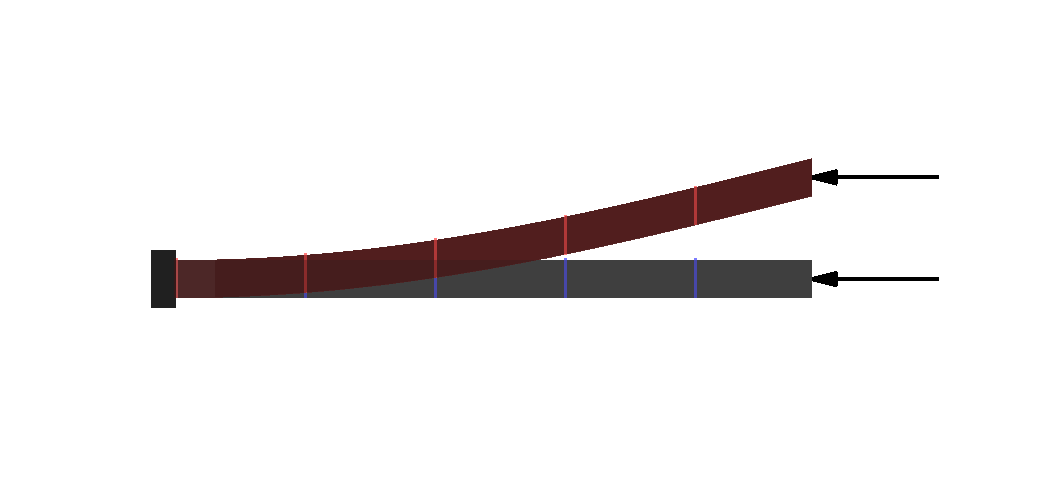
\includegraphics[width=0.49\linewidth]{Cantileverbeam.eps}}
	\subcaptionbox{悬臂梁分岔图\label{fig:Cantileverbeam Bifurcation}}
	{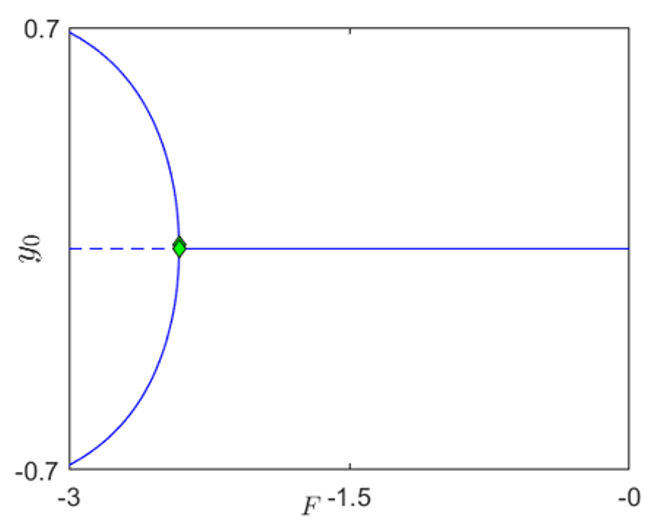
\includegraphics[width=0.49\linewidth]{2_9(2).png}}\\
	\caption{水平压力下的悬臂梁及其分岔图}
	\label{fig:水平压力下悬臂梁的失稳行为}
\end{figure}

下面算例为悬臂梁在非保守力作用下的失稳行为。一长度为$1$,宽厚比为$w/t=10$的悬臂梁,其两个主惯性轴方向的弯曲刚度分别为$0.7097$,$70.9731$,扭转刚度为1,拉伸刚度设为2000,用以约束节点与节点之间的相对距离。将该悬臂梁一端固支,而另一端自由,并在自由端施加跟随力(即压力的作用线方向始终与杆的切线方向保持共线),如图~\ref{fig:Follower Force}所示。当跟随力小于某一临界值时直线构形为稳定构形。当超过该临界值时,直线构形发生动力学失稳,并开始做周期性振荡。

本文结合离散弹性杆模型与COCO的“ep”工具箱求解该结构的平衡解并判断解的稳定性,在压力为$F=14.5$时存在一霍普夫分岔点,该霍普夫分岔点与利用公式\cite{elishakoff2001non}
\begin{equation}
	F_{\mathrm{cr}}=\frac{2\pi^2EI}{L^2}
\end{equation}
求得的理论解$F_{\mathrm{cr}}=14$相吻合。在分岔点之后原平衡构形失稳。另外,当压力$F=15$的情况下,用离散弹性杆进行动力学模拟,可以得到杆在无阻尼的情况下的振荡曲线,如图~\ref{fig:Vibration}。图~\ref{fig:Vibration}中纵坐标为悬臂梁自由端的垂直方向位移,横坐标为时间,在时间小于$1.5$秒时,悬臂梁由于无外界扰动,并未发生振动。但随着数值误差的积累,悬臂梁开始上下振动且振幅不断增大,当时间大于$3$秒时,振幅趋于稳定,悬臂梁此时在稳定的极限环上振动。该动力学模拟验证了结构在霍普夫分岔点之后原直线构形失稳,结构在稳定的极限环上振荡。
\begin{figure}
	\centering
	\subcaptionbox{跟随力作用下的悬臂梁\label{fig:Follower Force}}
	{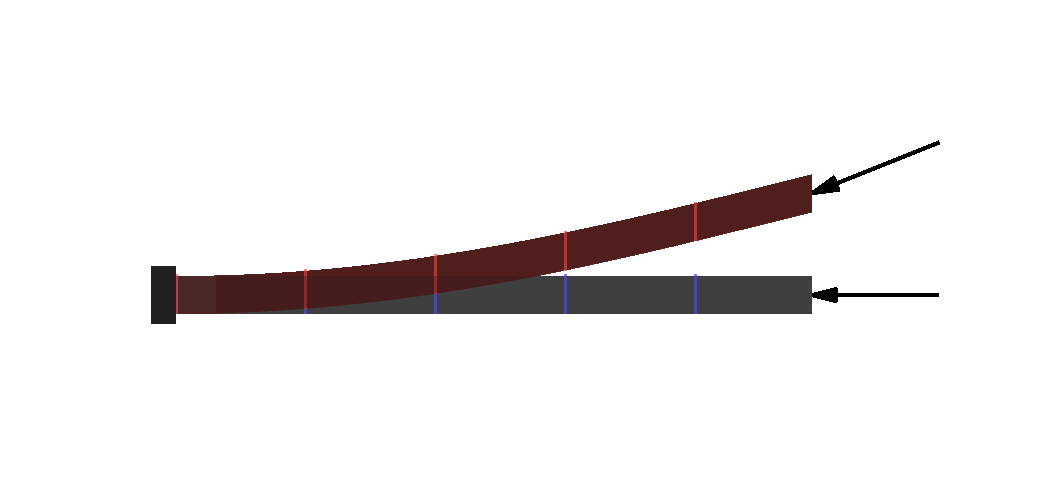
\includegraphics[width=0.49\linewidth]{follower forces.eps}}
	\subcaptionbox{悬臂梁自由端的位置随时间的变化关系\label{fig:Vibration}}
	{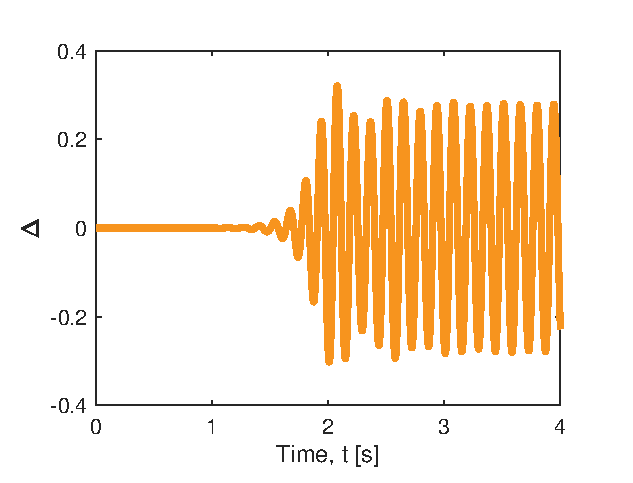
\includegraphics[width=0.49\linewidth]{Vibration.eps}}\\
	\caption{跟随力作用下的悬臂梁及其振动曲线}
	\label{fig:跟随力作用下的悬臂梁的失稳行为}
\end{figure}

通过上述两个算例,说明本文所设计的稳定性判断方法,不仅适用于对静力学稳定性的判断,同时也适用于动力学失稳的判断。
\subsection{剪切条带结构}
本算例中的结构为剪切条带\cite{yu2019bifurcations},其两端固支,长度为$1$。在压力作用下,当压力超过某一临界值时,条带会发生屈曲。继续施加水平压力,直到条带两端之间的距离为$0.5$,形成$\Omega$-型,如图~\ref{fig:Omega strip}所示。在此弯曲的$\Omega$-型上,施加平面外的位移$\Delta Y$,如图~\ref{fig:Sheraband_Shear}所示,结构展现出了复杂的分岔行为。
\begin{figure}
	\centering
	\subcaptionbox{未受载荷下的直线条带\label{fig:straight strip}}
	{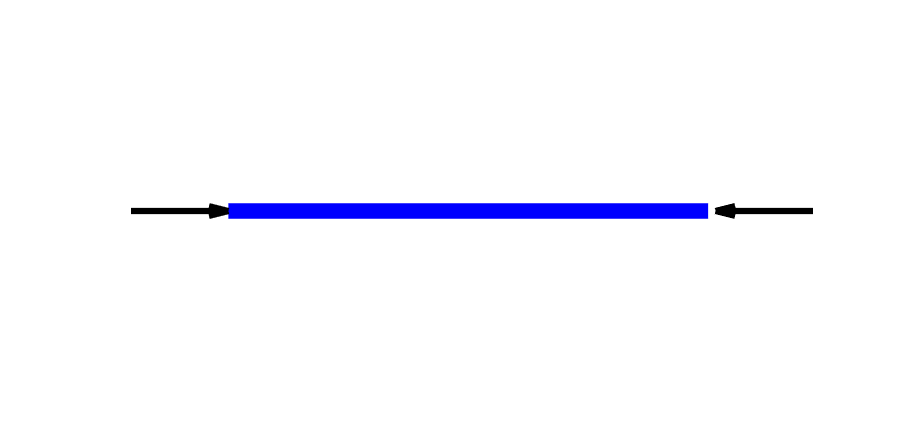
\includegraphics[width=0.49\linewidth]{Shearband_Straight.eps}}
	\subcaptionbox{$\Omega$构形条带\label{fig:Omega strip}}
	{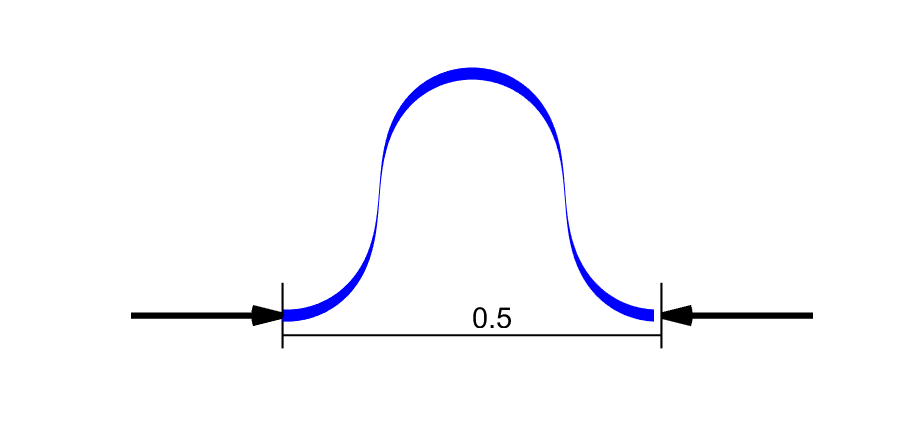
\includegraphics[width=0.49\linewidth]{Shearband_Omega.eps}}\\
	\subcaptionbox{受剪切位移后的条带\label{fig:Sheraband_Shear}}
	{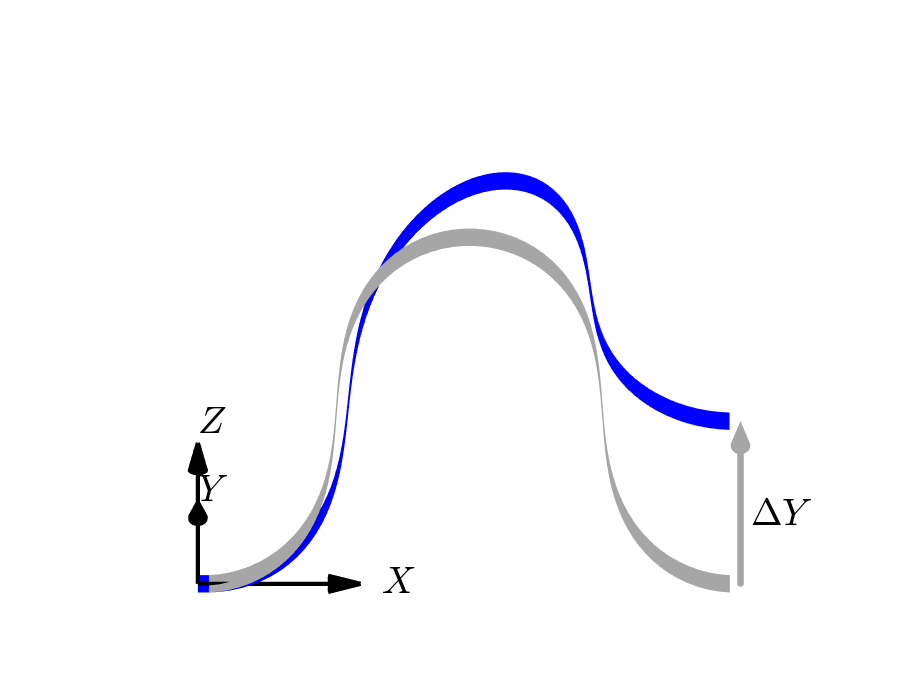
\includegraphics[width=0.7\linewidth]{Shearband_Shear.eps}}
	\caption{不同载荷下的剪切条带}
	\label{fig:不同载荷下的剪切条带}
\end{figure}

本算例中的条带长度为$1$,截面的宽厚比$w/t=20$。其两个主惯性轴方向的弯曲刚度分别为$0.6866$,$274.6550$,扭转刚度为$1$,拉伸刚度设为$2000$,用以约束节点与节点之间的相对距离。在利用离散弹性杆进行计算时,将该条带离散为$100$段。计算中将该弹性条带首端固支,即约束条带首端的两个节点坐标和第一离散段的相对转角;条带末端为滑动支座,即约束最后两个节点非轴向的位移以及最后一段离散弹性杆的相对转角,保持轴向位移自由。随后在末端施加水平方向的压力,当压力值达到$28.035$时,COCO检测到分岔点$BP$以及$SN$点,意味着该压力为条带失稳的临界压力;根据材料力学可知,两端固支的欧拉杆理论临界失稳压力为
\begin{equation}
	F_{\mathrm{cr}}=\frac{4\pi^2EI}{l^2}
\end{equation}
本案例中弯曲刚度为$0.6866$,相应的理论临界压力为$27.1$,与离散弹性杆模型所预测的临界压力相符。在该临界压力处,沿着分支进行延拓,直到压力为$37.565$,此刻条带被压缩为原长的一半,如图~\ref{fig:Omega strip}所示。随后将某端轴向位移的固定,在条带末端施加沿条带宽度的剪切位移$\Delta Y$。
\begin{figure}
	\centering
	\subcaptionbox{剪切条带的分岔图\label{fig:Shearband_Bifurcation}}
	{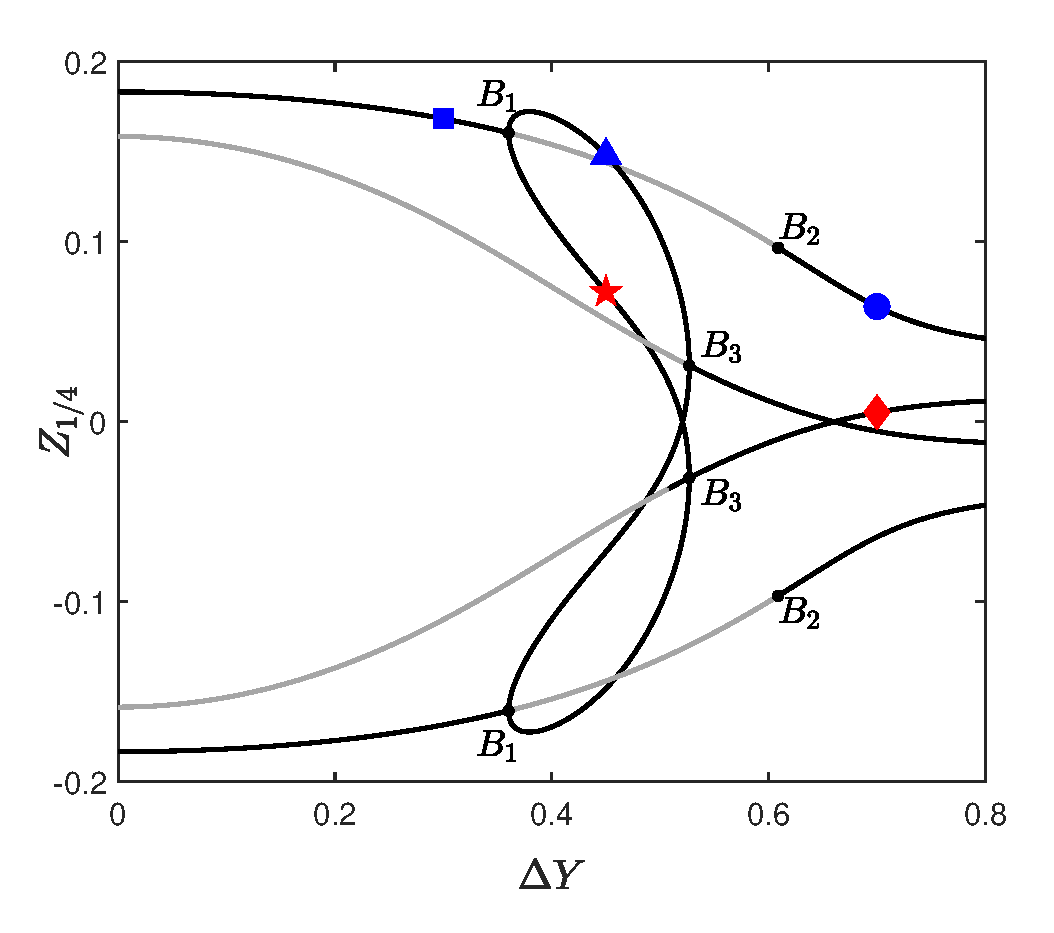
\includegraphics[width=0.8\linewidth]{Shearband_Bifurcation.eps}}\\
	\subcaptionbox{剪切位移为0.36时的稳定构形\label{fig:Shearband_0.36}}
	{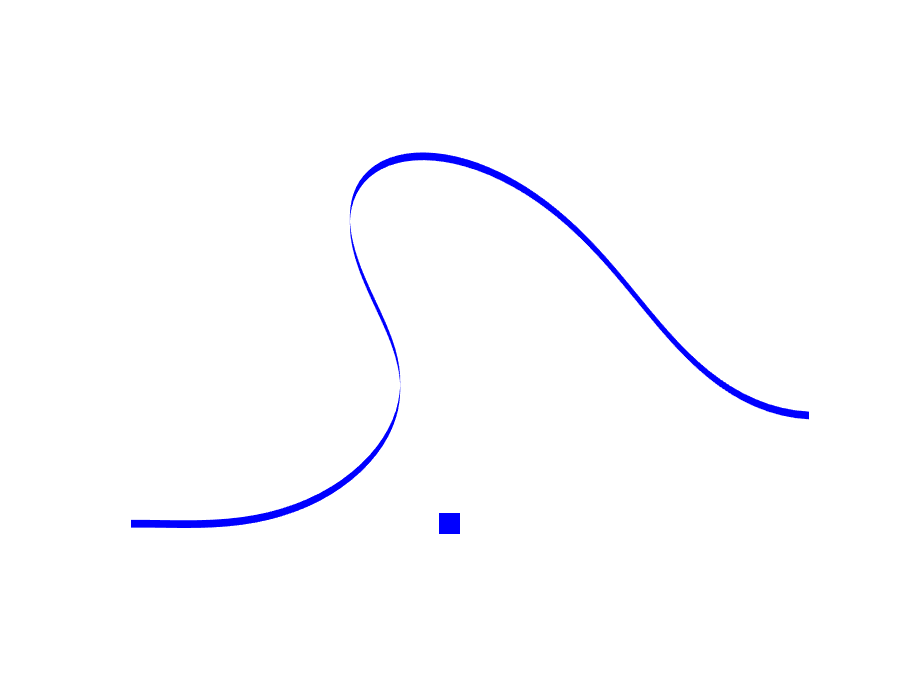
\includegraphics[width=0.3\linewidth]{Shearband_0.36.eps}}
	\subcaptionbox{剪切位移0.45时的稳定构形\label{fig:Shearband_0.45}}
	{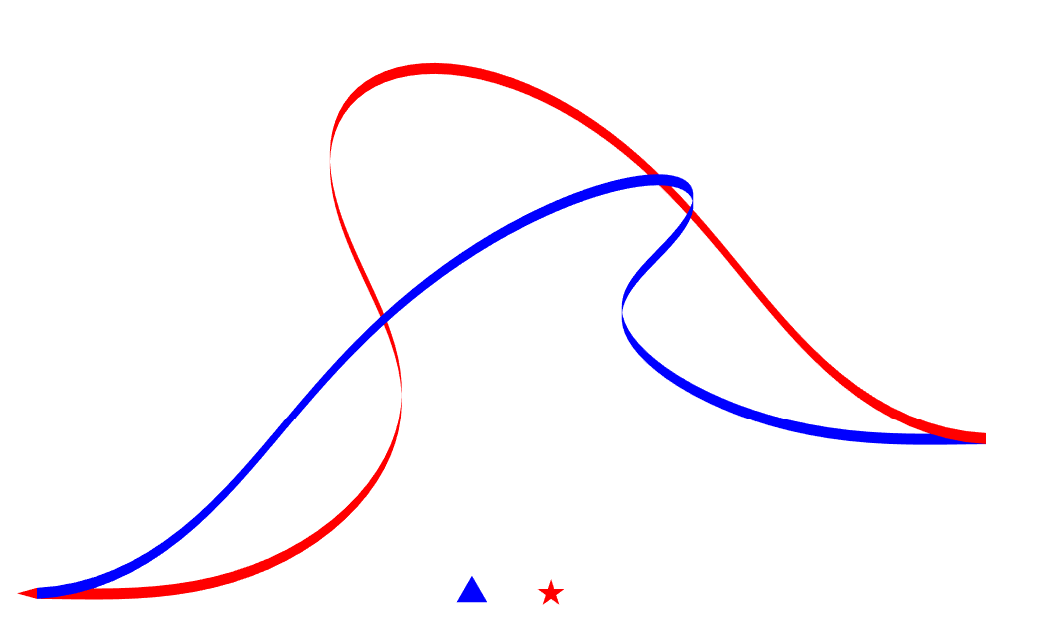
\includegraphics[width=0.3\linewidth]{Shearband_0.45.eps}}
	\subcaptionbox{剪切位移为0.7时的稳定构形\label{fig:Shearband_0.7}}
	{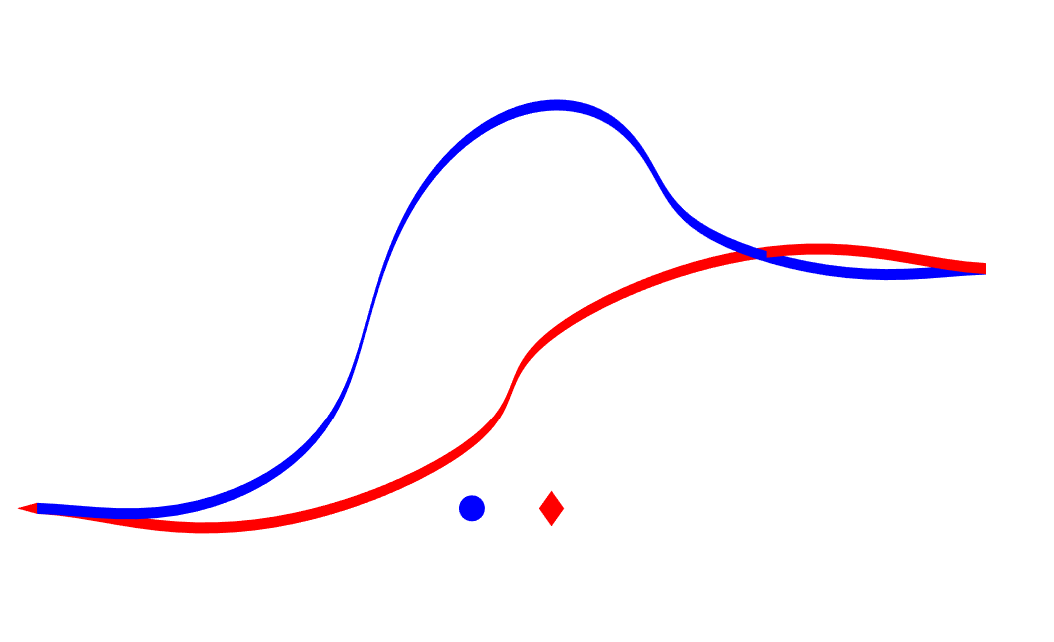
\includegraphics[width=0.3\linewidth]{Shearband_0.7.eps}}
	\caption{剪切条带的分岔图及相应的条带构形}
	\label{fig:剪切条带的分岔图及相应的条带构形}
\end{figure}

图~\ref{fig:Shearband_Bifurcation}为受剪切条带的分岔图,其中横坐标为延拓参数,为沿条带宽度方向($Y$方向)的剪切位移;纵坐标为条带四分之一弧长处的$Z$方向坐标,用于区分不同的平衡分支。以$\Omega$构形为延拓起点,对应图~\ref{fig:Shearband_Bifurcation}中$\Delta Y=0$时的最上侧曲线,当剪切位移逐渐增大并穿过分岔点$B_1$(对应剪切位移为$0.36$)时,同时存在一个SN点,存在一个特征值由负穿过零点变为正,意味着该平衡分支在分岔点$B_1$后失稳。该分支的解在经过分岔点$B_2$(对应剪切位移为$0.608$)时,同时穿过一SN点,存在一个正特征值穿过零点变为负数,该平衡解分支由非稳定状态重新变为稳定状态。从分岔点$B_1$向分支进行延拓,该分支形成一个闭环,整个闭环在延拓过程中无SN点的出现,因此整个分支为稳定解。在分支上存在分岔点$B_3$(对应剪切位移$0.5268$),从该分岔点延拓的分支中,存在一个SN点,将该分支分为稳定部分(剪切位移大于$B_3$)与非稳定部分(剪切位移小于分岔点$B_3$)。图~\ref{fig:Shearband_0.36},~\ref{fig:Shearband_0.45}和图~\ref{fig:Shearband_0.7}展示了部分稳定平衡分支上对应的条带构形,分别对应剪切位移为$0.36$,$0.45$,$0.7$下的稳定平衡构形。

\citet{yu2019bifurcations}利用各向异性杆模型对剪切条带结构进行了分岔分析,并通过实验对其数值计算结果进行了验证。另外,该文章还研究了条带宽厚比对分岔行为的影响。但该文章并未提出一种稳定性判定方法,来验证该结构各个平衡分支的稳定性。本文利用离散弹性杆模型就典型条件(即无宽厚比为$20$)下的剪切条带进行了分岔研究,结果与该文章结果\cite{yu2019bifurcations}吻合很好,包括分岔点位置与各分支解对应的条带构形。另外,本文中使用的稳定性判断准则很好地预测了所有平衡分支的稳定性。该算例说明了本文中提出的稳定性判断准则可以很好地应用于具有复杂分岔行为的结构稳定性判断。
\subsection{发卡结构}
本算例中所研究的结构为类似于图~\ref{fig:hair clips}所示的发卡的双稳态结构,称为Bigon,如图~\ref{fig:bigon}所示。该结构是由两根细长条带在首尾两端相互连接而成的结构。该算例代表了一类多杆系统,比如网状结构\cite{huang2022buckling},多根初始曲率不同的杆依次连接而成的杆件系统\cite{shi2025double}。通过该算例,可以验证本文所提出的稳定性测试方法在复杂杆系统中的适用性与有效性。
\begin{figure}
	\centering
	\subcaptionbox{发卡\label{fig:hair clips}}
	{\includegraphics[width=0.45\linewidth]{发卡.pdf}}
	\subcaptionbox{双条带构成的Bigon结构\cite{yu2021numerical}\label{fig:bigon}}
	{\includegraphics[width=0.45\linewidth]{Bigon图.pdf}}
	\caption{发卡结构与Bigon}
	\label{fig:bigon构形}
\end{figure}

该结构的具体组成过程如图~\ref{fig:Fabrication of Bigon}所示:两根长度为$l$,截面的宽厚比为$w/t=2$的细长杆首末两端固接在一起,两杆端部的切线所构成的夹角为$\gamma$,且首末两端的夹角$\gamma$保持相同。在利用离散弹性杆模型具体计算过程中,两个主惯性轴方向的弯曲刚度分别为$0.9693$,$3.8773$,扭转刚度为$1$,拉伸刚度设为$2000$,用以约束节点与节点之间的相对距离。
\begin{figure}
	\centering
	\includegraphics[width=0.8\linewidth]{Fabrication of Bigon.pdf}
	\caption{Bigon的组装过程\cite{yu2021numerical}}
	\label{fig:Fabrication of Bigon}
\end{figure}

在具体计算过程中,在两细长条带的$0$端,图~\ref{fig:Bigon_First order}所示,施加固支边界条件,即分别固定两杆前两个节点坐标以及第一个离散段上相对转角,该固接边界条件用来固定结构在空间中的位置。另一个端为固接边界条件。考虑到在$\gamma=0^\circ$(两杆处于未变形状态)处,末端两个连接单元构成的离散杆单元具有$180$度的拐角(相邻离散段之间共线且方向相反),根据离散曲率的定义式\eqref{eq:Discrete Curvature}无法定义该状态下的离散曲率因而无法直接利用前文所述的施加固接条件的方法。为此本文在计算过程中,以两杆弯曲为半圆弧时的状态(即$\gamma=180^\circ$)作为参数延拓的起点,延拓过程中逐渐减小角度$\gamma$。
\begin{figure}
	\centering
	\subcaptionbox{一阶屈曲模态\label{fig:Bigon_First order}}
	{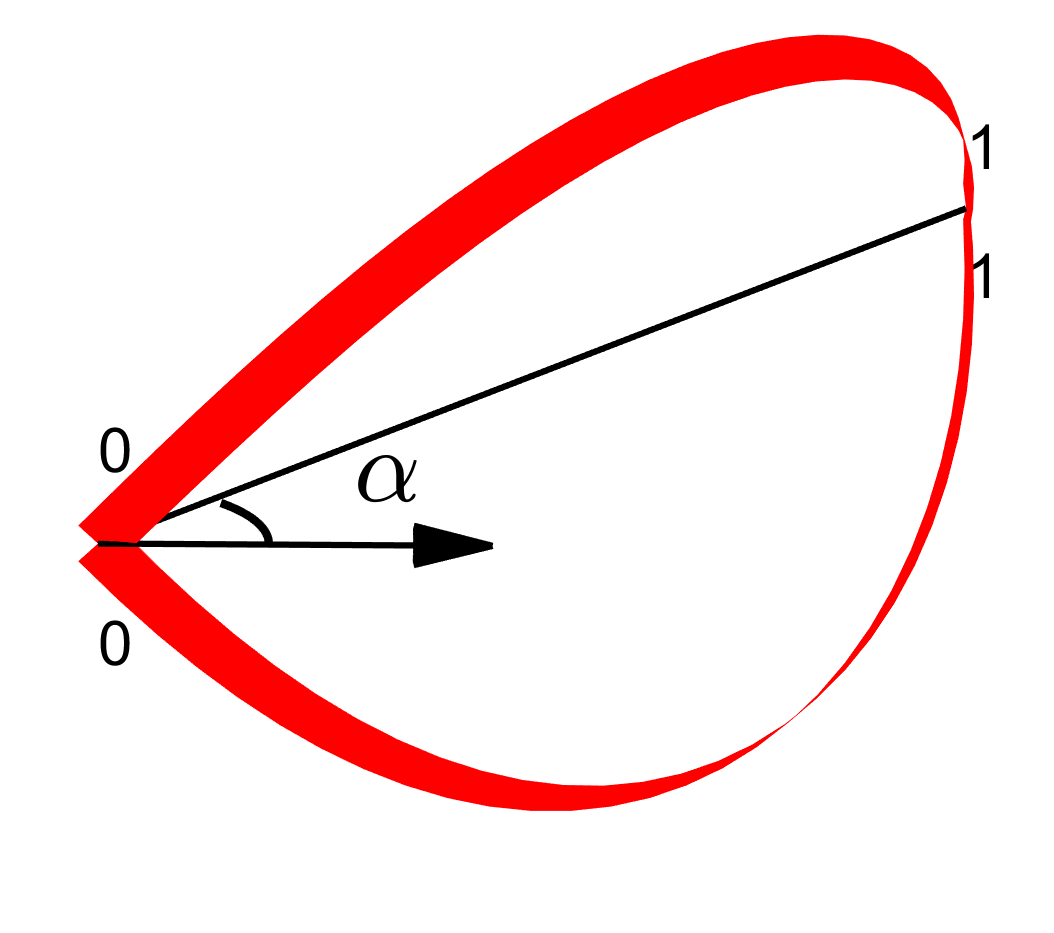
\includegraphics[width=0.4\linewidth]{Bigon_First order.eps}}
	\subcaptionbox{二阶屈曲模态\label{fig:Bigon_Second order}}
	{
\includegraphics[width=0.4\linewidth]{Bigon_Second_order.eps}}
	\caption{Bigon的一阶屈曲模态与二阶屈曲模态}
	\label{fig:Bigon的一阶屈曲模态与二阶屈曲模态}
\end{figure}
\begin{figure}
	\centering
	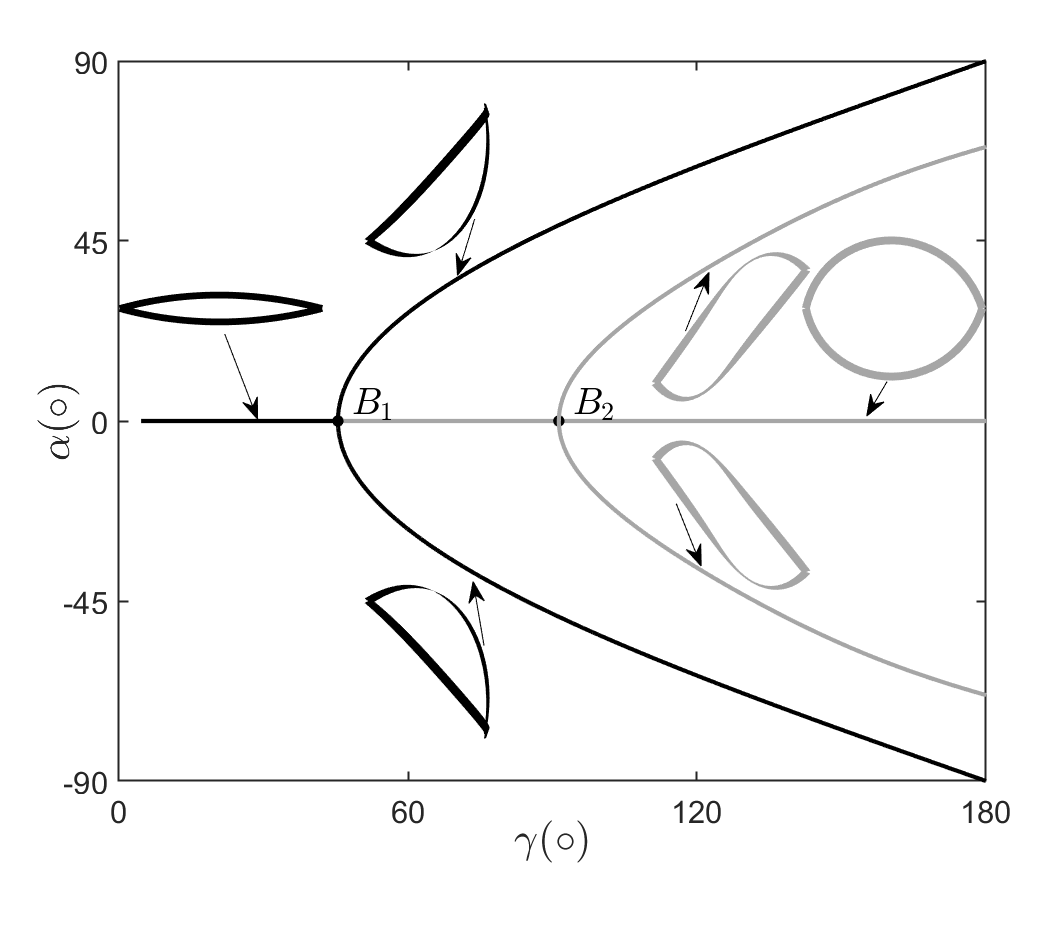
\includegraphics[width=0.7\linewidth]{Bigon_bifurcation.eps}
	\caption{Bigon分岔图}
	\label{fig:Bifurcation digram of Bigon}
\end{figure}

图~\ref{fig:Bifurcation digram of Bigon}展示了bigon的分岔图,其中,延拓参数为$\gamma \in \left[0,180^{\circ} \right]$,即两杆端部切线所构成的夹角。这里通过角度$\alpha$来区分不同的平衡分支,其中$\alpha$是由连接$0$端和$1$端的弦线,与两杆在$0$端的两个切线构成的夹角的角平分线构成的夹角。如图~\ref{fig:Bigon_First order}所示。在分岔图~\ref{fig:Bifurcation digram of Bigon}中横坐标为延拓参数$\gamma$,纵坐标为夹角$\alpha$。在分岔点$B_1$之前(张角$\gamma<45.45^{\circ}$),纵坐标$\alpha$始终保持为零,结构并未发生面外屈曲,保持平面构形,对应图~\ref{fig:Bifurcation digram of Bigon}中最左侧构形。另外,在分岔点$B_1$之前,在任意平衡点处,系统的特征值中无实部为正的特征值,因此该平面构形为稳定构形。当张角$\gamma$超过$B_1$时,结构发生面外屈曲,对应分岔图~\ref{fig:Bifurcation digram of Bigon}中穿过$B_1$的上下对称的平衡分支,平衡分支的对称性是由Bigon本身的对称性决定的,该结构可以向平面外任意一侧弯曲,其屈曲构形为图~\ref{fig:Bifurcation digram of Bigon}中两个上下对称的黑色构形,该构形为结构的一阶屈曲模态,如图~\ref{fig:Bigon_First order}所示。而其在分岔点$B_1$之后分岔点$B_2$之前($45.45^{\circ}<\gamma<91.3176^{\circ}$)的平面平衡解中,系统存在一个具有正实部的特征值,因此,平面解变为不稳定解,用灰色直线表示。而屈曲构形对应的平衡解的特征值中无实部为正的特征值,因此为稳定解。而在分岔点$B_2$之后,平面平衡解对应的特征值中有三个实部为正的特征值,平面解仍为非稳定解。二阶屈曲模态为不稳定构形,如图~\ref{fig:Bigon_Second order}所示,对应图中经过$B_2$的上下对称的不稳定分支。

Yu等\cite{yu2021numerical}利用基尔霍夫杆模型对该结构进行了分岔分析,并利用实验的手段对各个平衡解进行了稳定性判断。但并未通过数值的手段给出该结构平衡解的稳定性信息。本文中利用离散弹性杆模型结合分岔分析工具包COCO,对该结构进行了分岔分析并对所得平衡解进行稳定性判断。本文结果(包含分岔点位置以及稳定性判断结果)与Yu等\cite{yu2021numerical}的结果吻合良好,说明了该稳定性判断方法对多杆结构的有效性。

% !TeX root = ../sustechthesis-example.tex

\chapter{弹性蛇形条带的分岔及多稳态行为}
\section{引言}
本章中采用基尔霍夫杆模型对蛇形结构进行力学建模,并运用分岔分析工具包COCO对该模型进行了系统地分岔分析。同时,基于前一章节所设计的稳定性分析方法对所获得的平衡分支进行稳定性判定。此外,为确保数值分析结果的准确性与可靠性,本文通过实验手段对数值结果进行了实证验证。另外,本文针对具有不同单元数的蛇形条带,研究了该结构的多稳态特性。本章的结构安排如下:第一节首先给出弹性蛇形条带的几何描述,并指出其中关键的三个几何参数。在此基础上,对弹性蛇形条带进行力学建模,为后续的分岔分析奠定基础。最后,介绍实验所用的装置与弹性蛇形条带实物。随后的几节分别展示并分析单单元蛇形条带分岔图及多单元蛇形条带分岔图。其中,针对单单元蛇形条带,本文解释了其不同屈曲模态顺序交换及稳定性交换的数学机理——多重特征值分岔(double-eigenvalue bifurcation)。另外,本文针对不同单元的蛇形条带研究了该结构的多稳态特性。最后一节详细介绍了研究该结构多稳态特性所用的方法以及所得结果。
\section{弹性蛇形条带的建模与实验}
\subsection{弹性蛇形条带的几何描述及力学建模}
本小节给出弹性蛇形条带的几何描述。蛇形条带是由直线条带和半圆弧条带交替连接而成的细长结构,如图~\ref{fig:Serpentine_Schematics}所示,图中蛇形条带为双单元蛇形条带,一个蛇形条带单元的起始边界定义为图中条带最左端,终止边界为图中虚线位置,共由五个段构成,从左到右依次为长度为$l_2/2$的直线条带,上半圆弧状条带,长度为$l_2$的直线条带,下半圆弧以及长度为$l_2/2$的直线条带,本文中用$n_c$来表示蛇形条带的单元个数。条带的截面宽度用$w$表示,厚度用$t$来表示。本章中截面宽厚比$w/t$总取$10$。用无量纲化的参数$\alpha=l_2/l_1$来刻画结构的高度。本文主要研究在结构在拉伸位移载荷下的分岔行为。拉伸载荷大小用无量纲的拉伸位移$p=D_x/H$来刻画。在最左侧条带初始端$s=0$处的材料标架三个轴$\mathbfit{d}_1$,$\mathbfit{d}_2$,$\mathbfit{d}_3$分别沿着条带截面的宽度方向,厚度方向以及切线方向且三个坐标轴分别与全局坐标系的$\mathbfit{x}$,$\mathbfit{y}$,$\mathbfit{z}$轴共线。
\begin{figure}
	\centering
	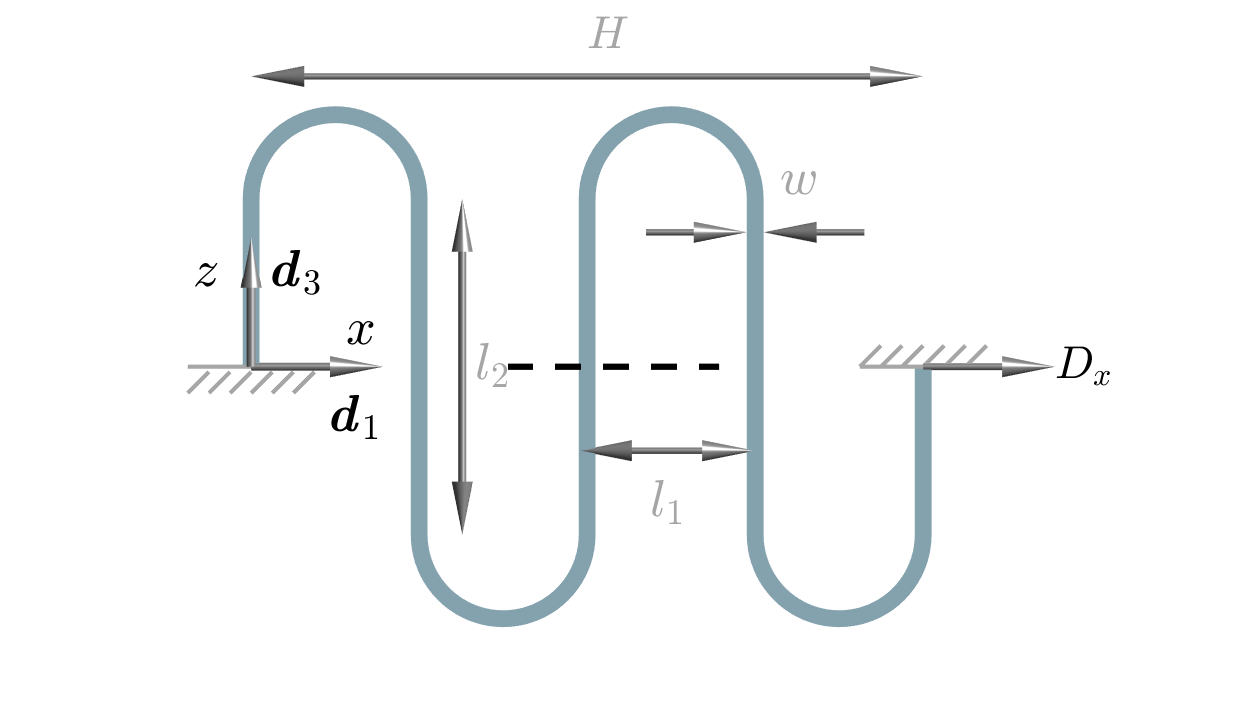
\includegraphics[width=0.6\linewidth]{Serpentine_Schematics}
	\caption{未变形时的双单元蛇形条带}
	\label{fig:Serpentine_Schematics}
\end{figure}

下面介绍如何用基尔霍夫杆模型来建立蛇形条带的力学模型。直线段与圆弧段的连接处的面内曲率不连续(圆弧段曲率为一个非零常数,而直线曲率保持为零),而基尔霍夫杆模型要求杆的曲率连续。因此需要在蛇形条带曲率不连续的地方进行分段,分别为每段条带建模并通过相应的连接条件将段与段之间相互连接。对于每一分段,根据式\eqref{eq:ToTle Equation}给出其控制方程。该方程中需要确定三个参数,分别为杆的长度$l$以及初始Darboux向量在材料坐标系$d_1$,$d_2$方向的分量$\kappa_{10}$,$\kappa_{20}$。对于杆长,这里将半圆弧段的条带长度设为1,作为单位来对其他分段长度进行无量纲化。设无量纲的结构高度为$\alpha$,那么一个单元中第一直线段与最后直线段的长度$l=\alpha/\pi$,中间直线段长度$l$为$2\alpha/\pi$。所有直线段的初始Darboux向量分量均为零。上半圆弧的Darboux向量的分量为$\kappa_{10}=0$,$\kappa_{20}=1/\pi$,而下半圆弧的Barboux向量对应的分量为$\kappa_{10}=0$,$\kappa_{20}=-1/\pi$。

对于单单元蛇形结构($n_c=1$)而言,共有五小段,每一分段可列$14$个控制方程,总共有$70$个微分方程。为了求解该微分方程,需要给出相同数量的边界条件。由初始端的固支约束可给出七个边界条件
\begin{equation}
	\begin{gathered}
	x^1(0)=0;\quad y^1(0)=0;\quad z^1(0)=0\\
	q^1_1(0)=1;\quad q^1_2(0)=0;\quad q^1_3(0)=0;\quad q^1_4(0)=0
\end{gathered}
\end{equation}
式中上标表示变量所属的条带分段,本处表示第一段上的变量。前三个边界条件固定条带初始端的位置,与四元数有关的四个条件用来固定转角。而对于整个结构的末端,同样可以根据固支条件施加七个边界条件
\begin{equation}
	\begin{gathered}
		x^5(1)=(1+p)\times\left(\alpha\cdot\frac{4}{\pi}\right);\quad y^5(1)=0;\quad z^5(1)=0\\
		q^5_1(1)=1;\quad q^5_2(1)=0;\quad q^5_3(1)=0;\quad q^5_4(1)=0
	\end{gathered}
\end{equation}
$p$为无量纲化的拉伸位移载荷。

另外,还需要给出分段与分段之间的连接条件
\begin{equation}
	\begin{gathered}
		N^i_1(0)=N^{i-1}_1(1);\quad N^i_2(0)=N^{i-1}_2(1);\quad N^i_3(0)=N^{i-1}_3(1)\\
		\kappa^i_{1}(0)=\kappa^{i-1}_{1}(1);\quad \kappa^i_{2}(0)-\kappa^i_{20}(0)=\kappa^{i-1}_{2}(1)-\kappa^{i-1}_{20}(1)\\
		\tau^{i}(0)=\tau^{i-1}(1) \quad \mathbfit{q}^{i}(0)=\mathbfit{q}^{i-1}(1) \quad \mu^{i}(0)=\mu^{i-1}(1)\\
		x^i(0)=x^{i-1}(1);\quad y^i(0)=y^{i-1}(1);\quad z^i(0)=z^{i-1}(1)
	\end{gathered}
\end{equation}
上式中,在每一连接处给出了十四个连接条件。式中上标$i$代表第$i$段条带上方程的变量,$i$可以取$2$,$3$,$4$,$5$。函数变量$0$为条带的首端,$1$为条件的末端。前三个边界条件为力的连续性条件。第三到第六个等式代表力矩的连续性条件。第七个式子为转角连续条件,第八个式子为常变量$\mu$的连续条件。最后三个式子代表位移连续条件。一个单元的蛇形条带有四个连接点,每个连接点处可以给出十四个连续性条件,外加十四个两端的固支边界条件,共有七十个边界条件。因此,结合方程与边界条件,可以组成一个适定的两点边界值问题。对于多单元的蛇形条带,只需要分别列出控制方程并在单元与单元之间给出相应的连接条件即可。

\subsection{弹性蛇形条带的实验}
本文对蛇形条带的研究,除了数值计算外,还通过实验来对数值结果进行验证。本小节简要介绍实验所用的加载装置以及蛇形条带的实物样本。
\begin{figure}
	\centering
	\includegraphics[width=1\linewidth]{ExptSetup (1).pdf}
	\caption{实验加载装置}
	\label{fig:ExptSetup}
\end{figure}

加载装置如图~\ref{fig:ExptSetup}所示,该装置通过SolidWorks设计三维模型并利用3D打印技术制作实物,所使用的3D打印机的型号为Creality Ender-3 S1如图~\ref{fig:3Dprinter}。加载装置主要由三部分组成:三个脚架,滑槽以及夹持结构。脚架的主要目的包括:(1)为整个结构提供支撑,(2)在滑槽下方预留适当的缝隙以容纳滑槽与加持结构之间的固定螺钉的延伸端。滑槽总长为\SI{50}{cm},由于3D打印机的成型尺寸限制,该滑槽被分为三个独立段进行加工,各滑槽之间铆接在一起,并通过螺钉固定以保证滑槽的稳定性。为便于拉伸位移的测量,滑槽上表面贴有刻度尺。夹持系统由两个加持臂构成。左侧加持臂固定于滑槽起始端,用以实现条带初始端的固支边界条件。右侧夹持臂具备轴向移动功能,可沿滑槽导轨平移,用于施加位移载荷。夹持臂的设计具有以下特征:(1)底部设有标准螺钉孔,可与滑槽狭缝配合实现位置锁定。(2)加持臂最上方设计有夹具,蛇形条带的末端可放入该夹具狭缝并通过两个上下排布的螺钉夹紧固定。在蛇形条带首末两端延伸出两个长方形末梢,如图~\ref{fig:ExptSetup}中深蓝色蛇形条带所示,用来将蛇形条带固定于夹具上。考虑到蛇形条带末梢的高度不同(左低右高),为了适应不同高度的加持末梢,在设计加持臂时,左右加持臂的高度不同(左低右高),左侧加持臂高度为\SI{20.5}{cm},右侧加持臂高度为\SI{23}{cm}。
\begin{figure}
	\centering
	\subcaptionbox{3D打印机\label{fig:3Dprinter}}
	{\includegraphics[width=0.4\linewidth]{3Dprinter.JPG}}
	\subcaptionbox{激光切割仪\label{fig:Laster Cutting}}
	{\includegraphics[width=0.4\linewidth]{Laster Cutting.JPG}}
	\caption{实验所用设备}
	\label{fig:experimental device}
\end{figure}

如图~\ref{fig:ExptSetup}所示,在图左侧,实验装置中设置了两个对比状态:不透明夹具上蛇形条带为初始未加载构型,而半透明夹具上条带为拉伸载荷作用下的屈曲构型。
\begin{figure}
	\centering
	\subcaptionbox{$\alpha=1.5$,$n_c=1$\label{fig:Serpentine Sample1.5}}
	{\includegraphics[width=0.11\linewidth]{Serpentine Sample1.5.pdf}}
	\subcaptionbox{$\alpha=4$,$n_c=1$\label{fig:Serpentine Sample4}}
	{\includegraphics[width=0.11\linewidth]{Serpentine Sample4.pdf}}
	\subcaptionbox{$\alpha=3$,$n_c=2$\label{fig:2Serpentine Sample3}}
	{\includegraphics[width=0.23\linewidth]{2Serpentine Sample3.pdf}}
    \subcaptionbox{$\alpha=3$,$n_c=3$\label{fig:3Serpentine Sample3}}
    {\includegraphics[width=0.36\linewidth]{3Serpentine Sample3.pdf}}
	\caption{蛇形条带实物}
	\label{fig:Samples of serpentine}
\end{figure}

图~\ref{fig:Samples of serpentine}展示了四个具有不同单元个数和高度的蛇形结构。这些蛇形结构通过AutoCAD设计,并利用激光切割仪(型号为Epilog FusionEdge,如图~\ref{fig:Laster Cutting}所示)在PVC塑料板上切割出相应的蛇形条带。所有蛇形结构的实际厚度为$t=\SI{0.24}{mm}$,截面宽度为$w=\SI{2.4}{mm}$(保证宽厚比为10)。同时将半圆弧直径设计条带宽度的十倍($R=5w$),即$2R=\SI{24}{mm}$,以保证蛇形结构的细长特性以及细长杆模型的有效性。若半圆弧直径小于截面宽度的十倍,那么二维的弹性理论\cite{wang2023substantial,yang2017elasticity}更适合捕捉此类结构的非线性特性,本文只考虑蛇形结构在细长情况下的力学行为。根据无量纲化高度$\alpha$以及半圆弧直径,可以得到实际的结构高度。$\alpha=1.5$对应的结构高度为$l_2=\SI{36}{mm}$,$\alpha=4$对应的结构高度为$l_2=\SI{96}{mm}$,$\alpha=3$对应的结构高度为$l_2=\SI{72}{mm}$。


\section{单单元蛇形条带分岔分析}
由于平面外弯曲刚度远小于平面内弯曲刚度,蛇形结构在拉伸载荷下会发生面外屈曲。Zhang等\cite{zhang2013buckling}在对蛇形结构的研究中发现,对于单单元蛇形条带($n_c=1$),其一阶屈曲模态的空间构形与结构的高度$\alpha$有关,具体而言,对于$\alpha<2.4$时,其一阶屈曲模态构形的俯视图展现出了反对称性,如图~\ref{fig:S_Mode}所示,由于其形状类似于字母S,下文称该模态为S模态;对于$\alpha>2.4$时,其一阶屈曲模态构形的俯视图展现出了正对称性,如图~\ref{fig:M_Mode}所示,下文称该模态为M模态。
\begin{figure}
	\centering
	\subcaptionbox{S模态\label{fig:S_Mode}}
	{
\includegraphics[width=0.3\linewidth]{S_Mode.eps}}
	\subcaptionbox{M模态\label{fig:M_Mode}}
	{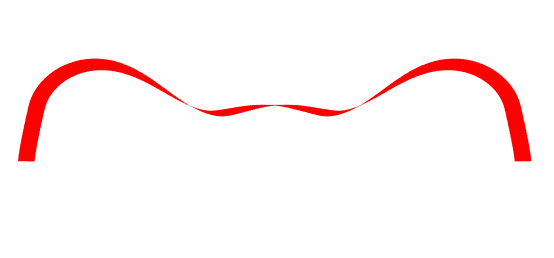
\includegraphics[width=0.3\linewidth]{M_Mode.eps}}
	\caption{单单元蛇形结构的一阶二阶屈曲模态}
	\label{fig:SM_Mode}
\end{figure}
针对这两类典型的蛇形结构,下面分别计算高度$\alpha=1.5$(代表一阶屈曲模态为S模态)以及高度$\alpha=4$(代表一阶屈曲模态为M模态)的单单元蛇形条带的分岔图,如图~\ref{fig:SerpentineNc1Aniso10}所示。

图~\ref{fig:SerpentineNc1Aniso10}(a-b),(d-e)分别为$\alpha=1.5$与$\alpha=4$的分岔图及其局部放大图。分岔图的横坐标对应于无量纲的位移载荷,纵坐标为图~~\ref{fig:SerpentineNc1Aniso10}(a)中蛇形结构上标记点$y_0$在拉伸载荷下的$y$方向位移。
从初始构形$D_x/H=0$出发,在结构的右端施加拉伸位移, 随着拉伸位移的增加,蛇形结构会发生面外屈曲使得原来的平面分支失稳(对应于$y_0=0$)。对于图~\ref{fig:SerpentineNc1Aniso10}(a)中$\alpha=1.5$的蛇形结构,在超临界分岔点$B_1$处,该结构发生屈曲,屈曲构形为一对稳定的S模态,(图~\ref{fig:SerpentineNc1Aniso10}(b)给出了该分岔点$B_1$处的放大图)。这一对S模态对应的两条平衡分支在超临界分岔点$B_3$后失稳,但在另一超临界分岔点$B_4$之后,该平衡分支重新稳定。在分岔点$B_4$之后,上下对称的一对S模态(对应图~\ref{fig:SerpentineNc1Aniso10}(c)中\bluesquare~/~\redsquare)始终保持稳定。除数值计算结果外,实验结果也表明:S模态除了在区间$B_3$,$B_4$之内,在其余位移载荷下均保持稳定。由分岔点$B_3$分岔得到的平衡分岔支与由分岔点$B_4$分岔出的平衡分支形成一个闭合的环,该闭合环上对应的模态(对应图~\ref{fig:SerpentineNc1Aniso10}(c)中\Brighttriangle~/~\Rrighttriangle~/~\Blefttriangle~/~\Rlefttriangle~)始终保持稳定,另外,该模态的空间构形并不具有对称性。在距分岔点$B_1$很近的后方,二次分岔点$B_2$出现并从该分岔点处分岔出一对平衡分支。该平衡分支在初始阶段其分支解为非稳定解,但在穿过亚临界分岔点$B_5$(考虑到分岔图的简洁性,这里没有展示从分岔点$B_5$分岔出的不稳定分支)之后,整个平衡分支变为稳定解,该稳定解为M模态(对应图~\ref{fig:SerpentineNc1Aniso10}(c)中~\Btriangle~/~\Rtriangle)。下面简要总结该蛇形结构在载荷不断增大时的行为,对于$\alpha=1.5$的蛇形条带,当位移载荷增大到分岔点$B_1$处,结构发生面外屈曲,屈曲模态为$S$模态。随着载荷进一步增加,原$S$模态在经过分岔点$B_3$之后,具有反对称特性的$S$模态分支失稳,结构沿$B_3$处分岔支变形(对应图~\ref{fig:SerpentineNc1Aniso10}(c)中\Brighttriangle~/~\Rrighttriangle~/~\Blefttriangle~/~\Rlefttriangle~),屈曲构形失去对称性。最后,进一步增大拉伸载荷,在经过分岔点$B_5$之后,构形又回到S模态对应的分支上并一直沿该分支变形上。
\begin{figure}[t]
	\centering
	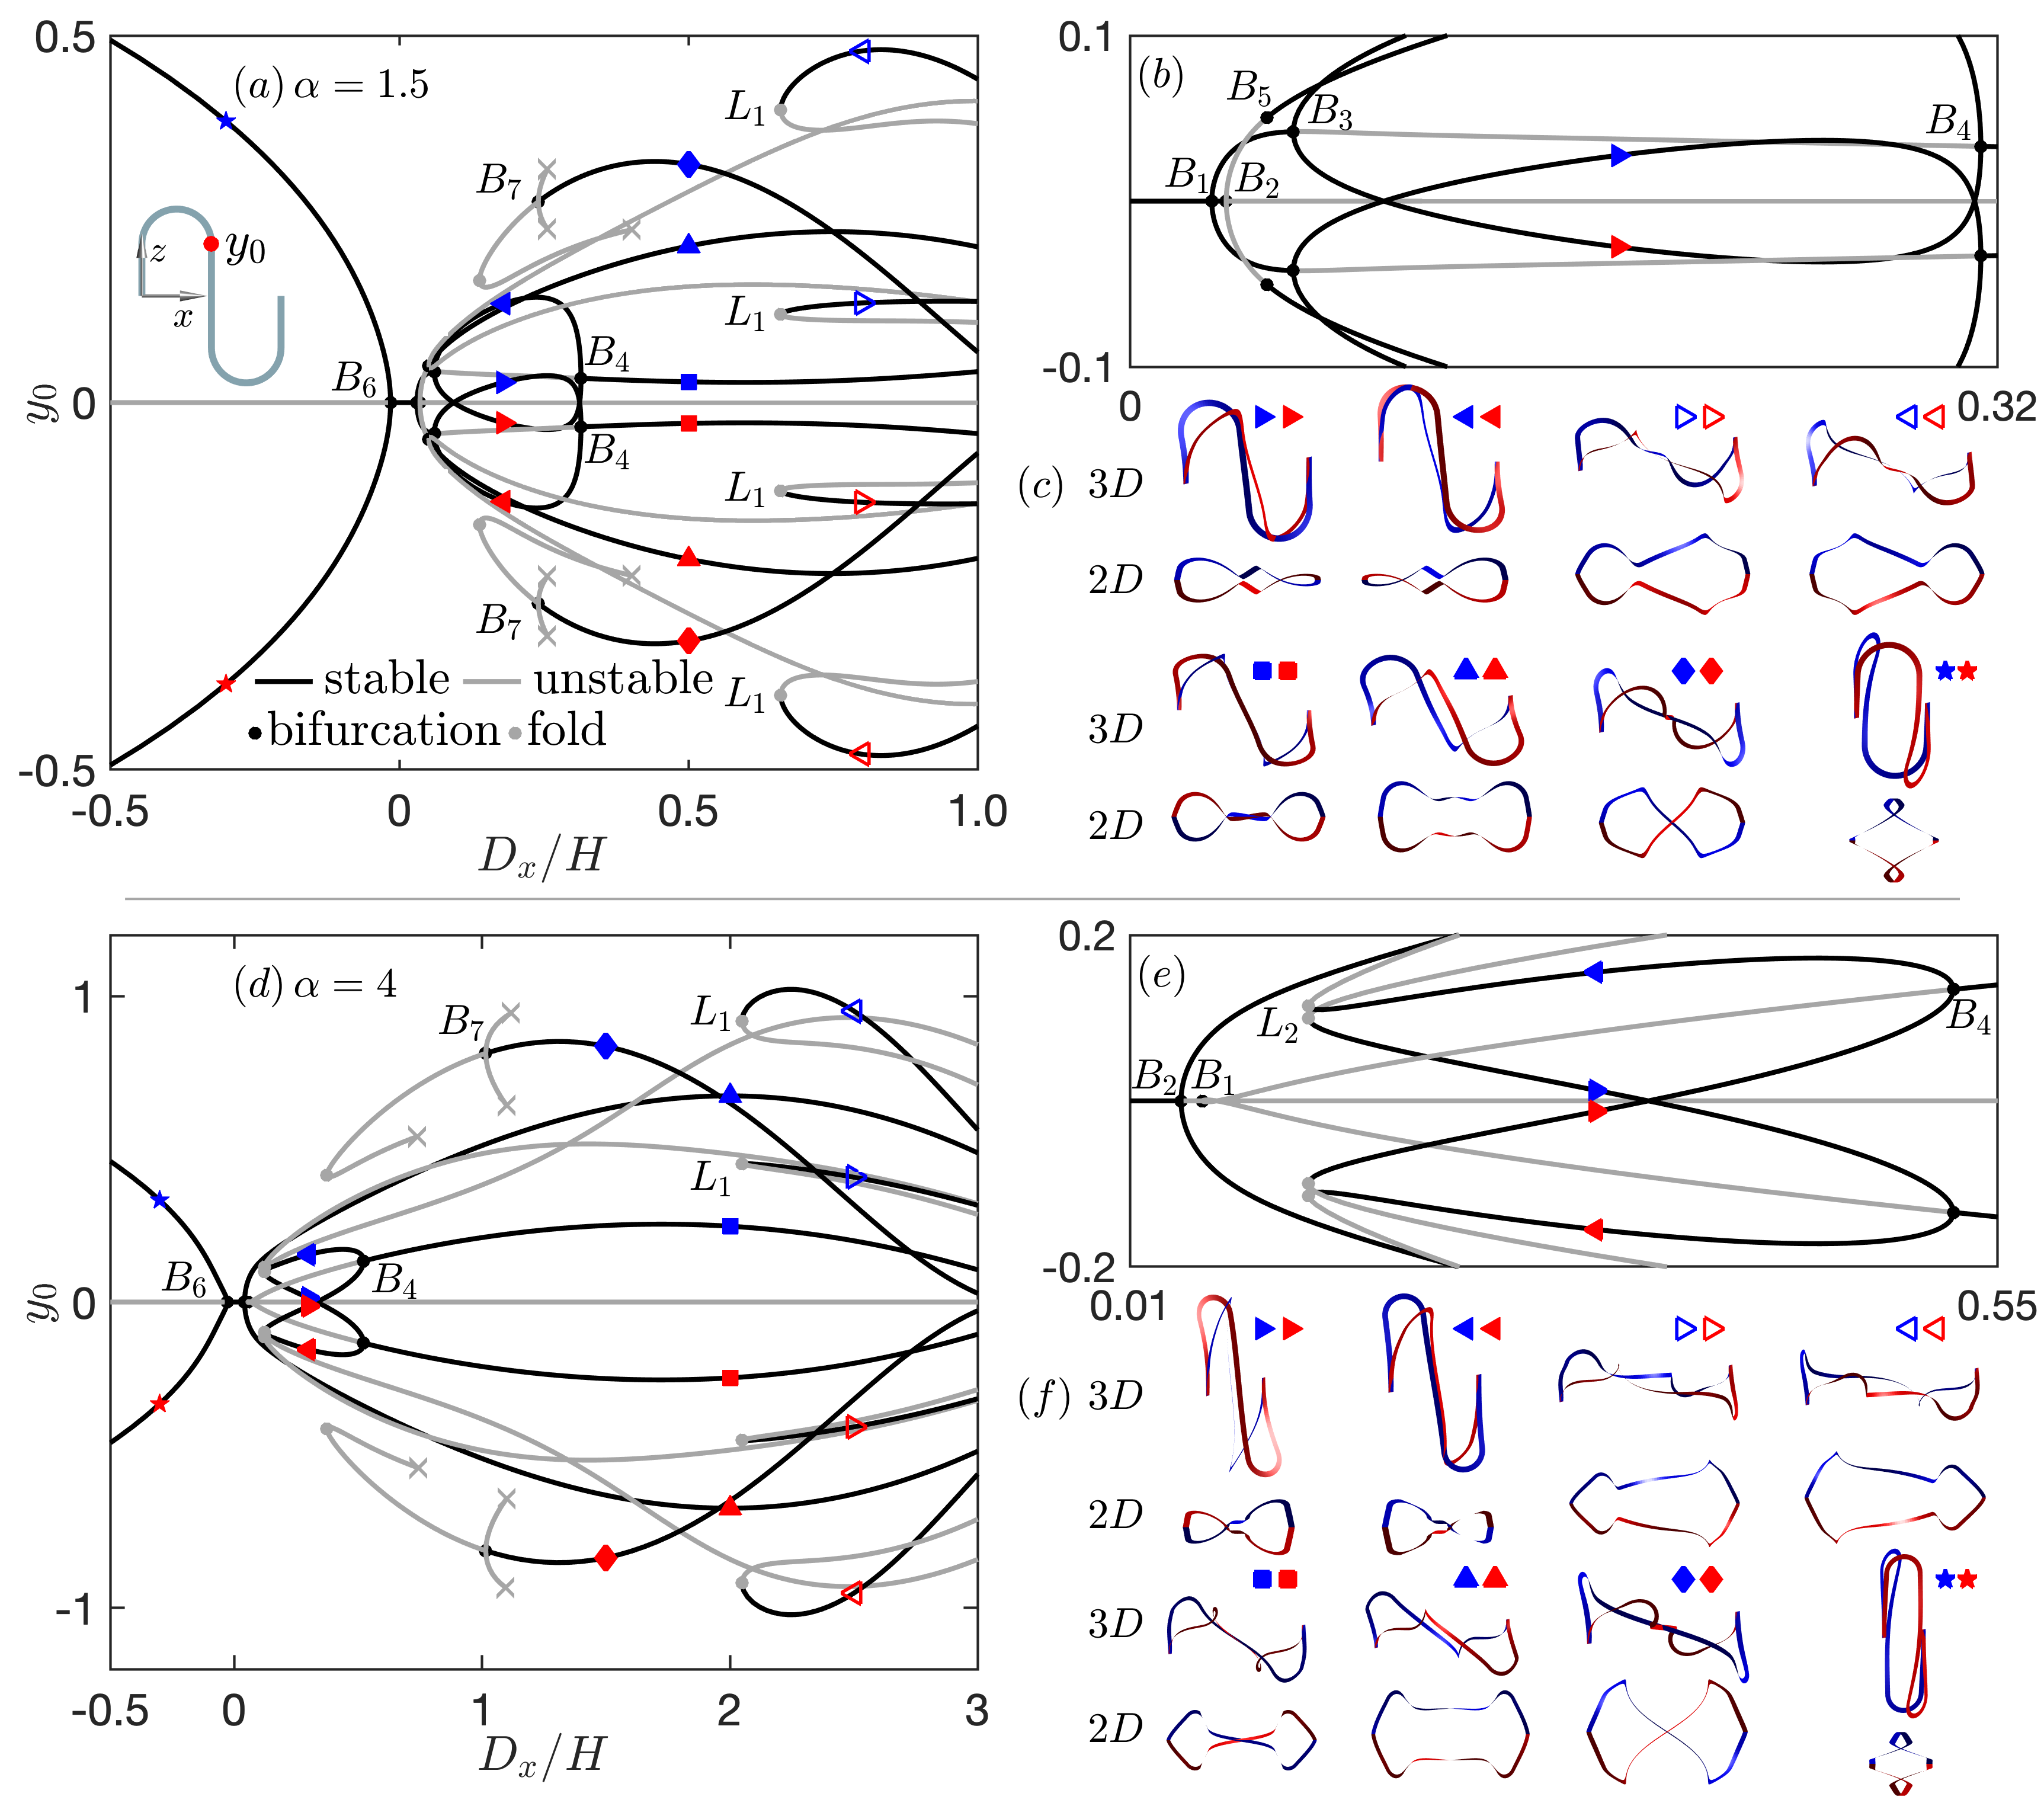
\includegraphics[width=1\linewidth]{SerpentineNc1Aniso10.png}
	\caption{不同高度的单单元蛇形结构的分岔图及对应分岔支的平衡构形。(a) $\alpha=1.5$的分岔图。(b) 图(a)的局部放大图。(c) 分岔图(a)中平衡分支对应的稳定构形。(d)  $\alpha=4$的分岔图。(e) 图(d)的局部放大图。(f) 分岔图(d)中平衡分支对应的稳定构形。}
	\label{fig:SerpentineNc1Aniso10}
\end{figure}

分岔图~\ref{fig:SerpentineNc1Aniso10}(a)中存在不与平面平衡分支$y_0=0$连接的其他稳定分支。其中一对这类孤立的分支为图~\ref{fig:SerpentineNc1Aniso10}(a)中(~\Rdiamond~/~\Bdiamond)中所标记的分支,该分支对应的解在亚临界分岔点$B_7$之后变为稳定解,该分支对应的构形同样为反对称构形(从俯视图观察)。另外,图~\ref{fig:SerpentineNc1Aniso10}(a)中\HBrighttriangle~/~\HRrighttriangle~/~\HBlefttriangle~/~\HRlefttriangle~标记的平衡分支同样不与平面解($y_0=0$)相连,且每一分支中存在一拐点$L_1$,意味着这些分支对应的稳定构形只有当载荷大于拐点$L_1$所对应的载荷才存在。在压缩位移载荷下($D_x/H<0$),蛇形结构同样会发生面外屈曲,当压缩位移超过超临界分岔点$B_6$时,蛇形结构发生面外屈曲,其屈曲模态为图~\ref{fig:SerpentineNc1Aniso10}(c)中~\Bstarshape~/~\Rstarshape。

图~\ref{fig:SerpentineNc1Aniso10}(d-e)为$\alpha=4$的蛇形结构的分岔图。相比于$\alpha=1.5$的分岔图,$\alpha=4$的分岔图中分岔点$B_1$和$B_2$的位置发生了交换,即分岔点$B_2$对应的载荷小于分岔点$B_1$对应的载荷,意味着随着载荷的增大,该蛇形结构会发生屈曲且其屈曲模态为一对M模态(对应图~\ref{fig:SerpentineNc1Aniso10}(f)中~\Btriangle~/~\Rtriangle~),而且该模态对应的分支解总为稳定解。分岔点$B_1$位于$B_2$之后不远处,从分岔点$B_1$分岔出的一对平衡分支在一开始为不稳定解,但经过超临界分岔点$B_4$之后,该分岔点变为稳定性解,对应着S模态(如图~\ref{fig:SerpentineNc1Aniso10}(f)中~\bluesquare~/~\redsquare~ 所示)。从分岔点$B_4$分岔出去的平衡分支(相应的稳定构形如图~\ref{fig:SerpentineNc1Aniso10}(f)中~\Brighttriangle~/~\Rrighttriangle~/~\Blefttriangle~/~\Rlefttriangle~所示),在一开始为稳定解,但经过拐点$L_2$之后该解失稳。在实际加载过程中,$\alpha=4$的蛇形条带在加载过程中,经过分岔点$B_2$之后,结构屈曲到M模态,并且在随后的加载过程中一直保持M模态。

类似于$\alpha=1.5$的蛇形结构,在$\alpha=4$的结构分岔图中同样存在不与平面平衡分支($y_0=0$)相连的解,包括一对上下对称的孤立分支,对应于图~\ref{fig:SerpentineNc1Aniso10}(f)中(~\Rdiamond~/~\Bdiamond)的构形,该分支对应的解在亚临界分岔点$B_7$之后变为稳定解。另外,图~\ref{fig:SerpentineNc1Aniso10}(c)中\HBrighttriangle~/~\HRrighttriangle~/~\HBlefttriangle~/~\HRlefttriangle~对应的平衡分支同样不与平面解对应的分支相连,且每一分支中存在一拐点$L_1$,意味着这些分支对应的稳定构形只有当载荷大于拐点$L_1$时对应的载荷才存在。

上述分析给出了两类典型高度的单单元蛇形结构的分岔图。Zhang等\cite{zhang2013buckling}发现当$\alpha<2.4$时,结构的屈曲模态为S模态,而当$\alpha>2.4$时,结构的屈曲模态为M模态。本节首先通过实验验证了同样的现象。随后,本文通过分岔分析对这一现象给出了解释:不论蛇形结构的高度,在足够的拉伸载荷下S模态和M模态均存在。但其出现的顺序不同,对于高度较小的蛇形结构,S模态出现所需的位移载荷小于M模态所需的载荷,即S模态为一阶屈曲模态,而M模态为二阶屈曲模态。而对于结构高度较大的蛇形条带,M模态为一阶屈曲模态,而S模态为二阶屈曲模态。

\section{多重特征值分岔}
上一节给出了两类典型高度的蛇形结构的分岔图,从图~\ref{fig:SerpentineNc1Aniso10}可以看到屈曲模态的交换对应于分岔点$B_1$,$B_2$的位置交换。另一方面,稳定性交换对屈曲模态的交换也至关重要。在$\alpha=1.5$的分岔图~\ref{fig:SerpentineNc1Aniso10}(a)中,一阶屈曲模态,即从$B_1$分岔点分岔出的平衡分支,在分岔点$B_1$附近为稳定解。二阶分岔点$B_2$分岔出的平衡分支在一开始为非稳定解。而对于$\alpha=4$的分岔图~\ref{fig:SerpentineNc1Aniso10}(d)具有相反的情况。从$B_1$分岔点分岔出的平衡分支,在分岔点$B_1$附近为非稳定解,分岔点$B_2$分岔出的平衡分支在一开始为稳定解。这种不同屈曲模态的稳定性交换,对屈曲模态交换至关重要,若不同分岔支上稳定性未发生交换,那么从分岔点$B_2$分岔出的分支为非稳定解,蛇形结构无法向非稳定分支延拓,因此不会屈曲为M模态,无法实现模态交换。本节将通过详细分析临界高度(不同模态交换刚好发生交换的高度)附近的分岔过程,揭示了不同屈曲模态对应分支的稳定性交换过程。
\begin{figure}
	\centering
	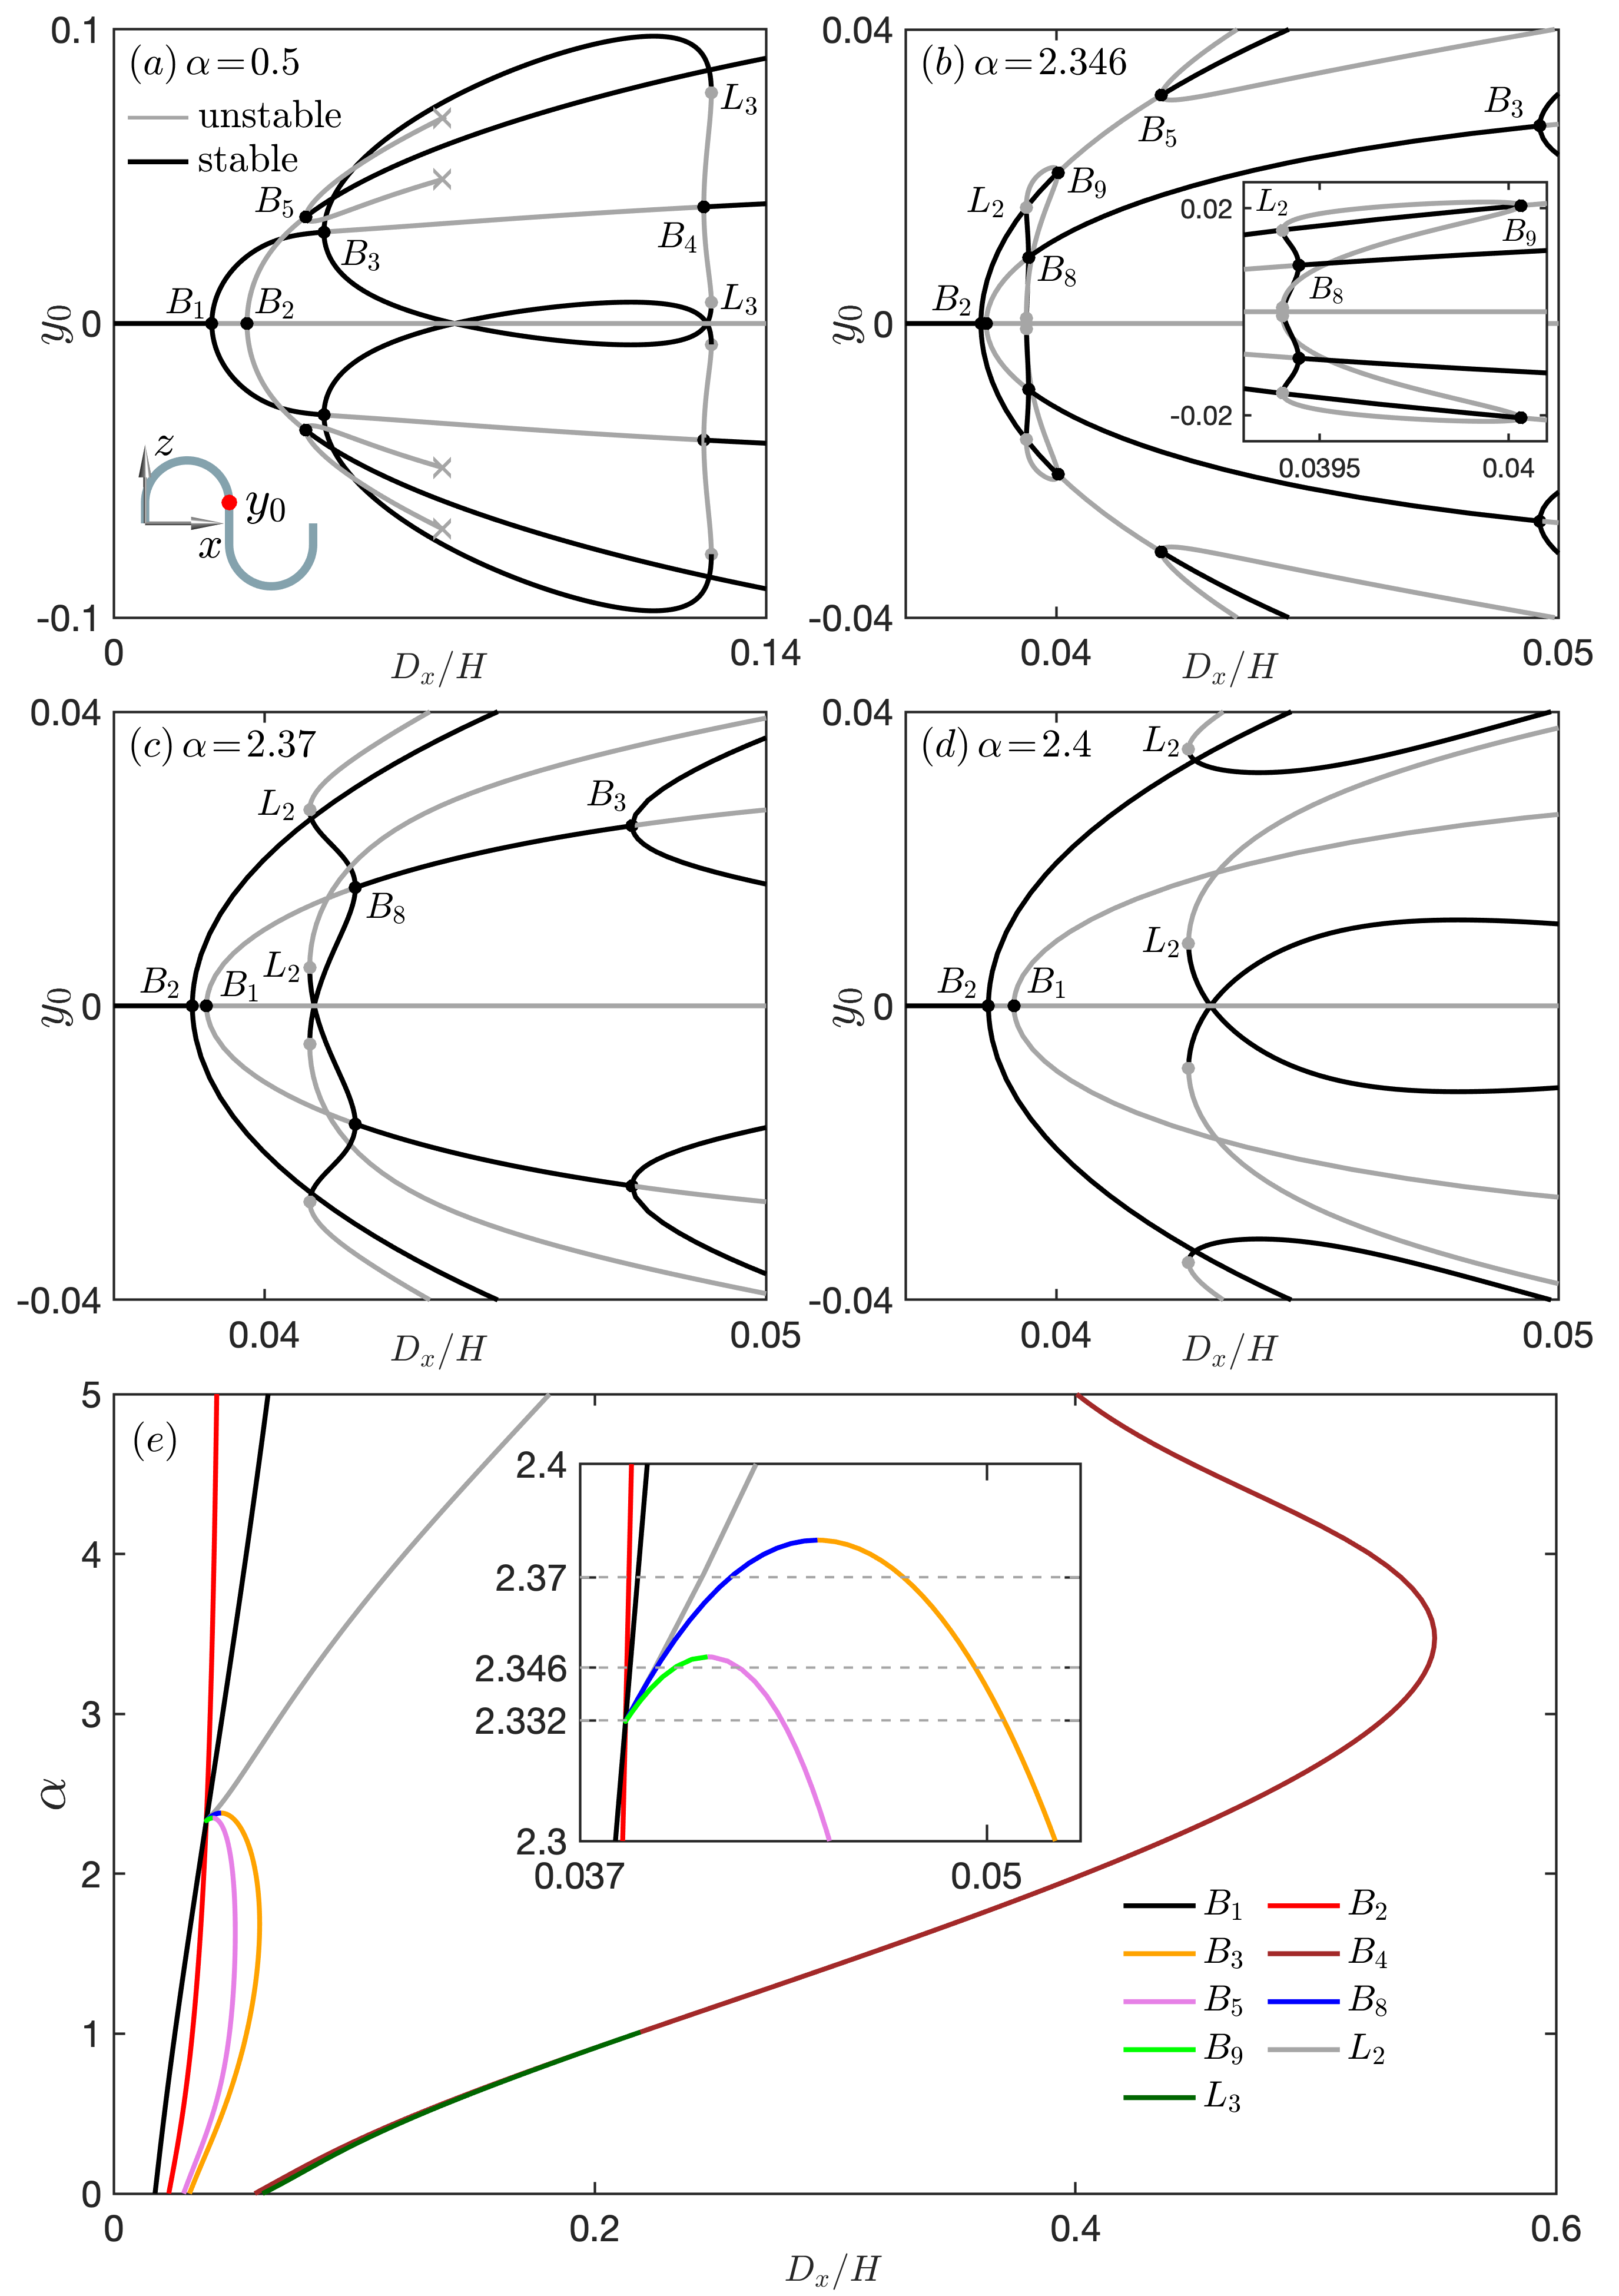
\includegraphics[width=1\linewidth]{SerpentineNc1Aniso10Phase.png}
	\caption{单单元蛇形条带不同屈曲模态交换的过程。(a-d) 不同高度$\alpha$下的分岔图。(e) 图(a-d)中分岔点随高度变化的轨迹。}
	\label{fig:SerpentineNc1Aniso10Phase}
\end{figure}

通过分岔分析软件AUTO 07P\cite{doedel2007auto}的双参数延拓功能可以计算绘制分岔点的轨迹曲线,图~\ref{fig:SerpentineNc1Aniso10Phase}(e)为分岔点的轨迹图,横坐标为相应分岔点的位置,纵坐标为无量纲的结构高度$\alpha$,图中黑色曲线为分岔点$B_1$随高度变化的轨迹,红色曲线为分岔点$B_2$沿高度变化的轨迹。在高度$\alpha=2.332$处时,两条轨迹线存在一交点,即分岔点$B_1$与分岔点$B_2$重合。该交点对应的高度为临界高度,高度大于该数值,结构在拉伸载荷下屈曲为M模态,低于该高度,结构会屈曲为S模态。该临界高度与Zhang等\cite{zhang2013buckling}所报道的$2.4$吻合。

在$\alpha=2.332$处,该系统为退化的情形,当$\alpha>2.332$时,两个二次分岔点$B_8$,$B_9$从$B_1$,$B_2$的交点处出现(对应于轨迹图~\ref{fig:SerpentineNc1Aniso10Phase}(e)的蓝色曲线和绿色曲线),为了更好地了解二次分岔点$B_8$,$B_9$的演化过程,本文绘制了$\alpha=2.346$下(对应于二次两个分岔点$B_8$,$B_9$同时存在的情形)的分岔曲线,如图~\ref{fig:SerpentineNc1Aniso10Phase}(b)所示。从图中可以看到二次分岔点$B_8$,$B_9$分别在$B_1$,$B_2$对应的分岔支上,$B_8$的出现使得$B_1$到$B_8$区间中原本稳定的平衡分支失稳,而$B_9$的出现使得$B_2$到$B_9$区间中原本不稳定的平衡分支获得稳定性。从轨迹图~\ref{fig:SerpentineNc1Aniso10Phase}(e)可以看出分岔点$B_8$,$B_9$从$B_1$,$B_2$的交点出发,分别逐渐向分岔点$B_3$,$B_5$靠近。随着$B_8$的靠近,$B_1$分岔出的平衡分支稳定区间($B_1$—$B_3$)逐渐失稳。而随着$B_9$的靠近,$B_2$分岔出的平衡分支非稳定区间($B_2$—$B_5$)对应的解逐渐变为稳定解。图~\ref{fig:SerpentineNc1Aniso10Phase}(b)只标记了$y_0>0$的二次分岔点,对于$y_0<0$的情况,同样也会存在相同的二次分岔点,上下两对分岔点$B_8$,$B_9$共同构成了一个闭合的环形分岔支。随着高度$\alpha$的减小,这个环形分岔支会逐渐缩小到最终与$B_1$,$B_2$的交点重合。

上述演化过程对应着一类典型的分岔行为——多重特征值分岔(double eigenvalue bifurcation),该分岔行为存在于各类力学现象中\cite{bauer1975multiple,tavener1988buckling,keener1979secondary}。当系统某一参数发生变化时,一个多重分岔点会分裂为两个主分岔点以及若干个二次分岔点\cite{bauer1975multiple}。在本文的情形中,$B_1$,$B_2$为主分岔点,$B_8$,$B_9$为二次分岔点。在$\alpha=2.332$下,$B_1$,$B_2$的交点处为多重特征值分岔点,随着$\alpha$增大,该多重特征值分岔点分裂为两个主分岔点$B_1$,$B_2$,以及两个二次分岔点$B_8$,$B_9$。而二次分岔点的出现促使不同分岔支发生稳定性交换。

从轨迹图~\ref{fig:SerpentineNc1Aniso10Phase}(e),当结构高度$\alpha$增加到某一数值之后,二次分岔点$B_9$与分岔点$B_5$融合(在某一高度处,绿色轨迹与紫色轨迹相连)。$\alpha=2.37$为融合之后的某一结构高度,其分岔图为~\ref{fig:SerpentineNc1Aniso10Phase}(c),图中可以看到分岔点$B_2$对应的分岔支上无二次分岔点$B_9$,$B_5$的出现,使得整个平衡分支对应稳定解。随着高度的进一步增加,二次分岔点$B_8$与分岔点$B_3$融合(在某一高度处,图~\ref{fig:SerpentineNc1Aniso10Phase}(e)中蓝色轨迹与橘色轨迹相连)。$\alpha=2.4$为融合之后的某一高度,其分岔图为~\ref{fig:SerpentineNc1Aniso10Phase}(d),图中可以看到分岔点$B_1$对应的分岔支上无二次分岔点$B_8$,$B_3$的出现,分岔点$B_1$分岔出的分支在分岔点$B_4$之前为非稳定解。
\section{多单元蛇形条带分岔行为}
前面两节对单单元蛇形结构进行了分岔分析并揭示了不同屈曲模态交换的数学机理。但在蛇形结构的实际应用中,多单元蛇形结构往往具有更广泛的应用场景。因此,本节考虑多单元蛇形结构的分岔行为,以$\alpha=3$,单元数$n_c=2$和$n_c=3$的蛇形结构为例进行分岔分析,类似的分析方法可以用于分析其余任意单元数,任意高度的蛇形结构。

图~\ref{fig:SerpentineNc2Nc3Aniso10Phase}给出了相应的数值计算结果。图~\ref{fig:SerpentineNc2Nc3Aniso10Phase}(a-d)分别展示了$n_c=2$,$\alpha=3$的分岔图,分岔图的局部放大图,分岔图中平衡分支对应的稳定构形,以及分岔图中分岔点随结构高度变化的轨迹图。类似于图~\ref{fig:SerpentineNc2Nc3Aniso10Phase}(a-d),图~\ref{fig:SerpentineNc2Nc3Aniso10Phase}(e-f)展示了$n_c=3$,$\alpha=3$的蛇形结构对应的数值计算结果。对于这两种不同单元数的情况,蛇形结构在经过超临界分岔点$B_1$之后会发生屈曲,其屈曲模态均为S模态(对应图~\ref{fig:SerpentineNc2Nc3Aniso10Phase}(c),(g)中~\Bdiamond~所标记的构形),分岔点$B_1$之后存在第二个分岔点$B_2$,从分岔点$B_2$分岔出的两个分岔支在初始时为不稳定的平衡解,但在该分支上存在一对(上下分支各一个)亚临界分岔点$B_3$,在该分岔点之后,从分岔点$B_2$分岔出的两个分支变为稳定平衡解,对应的平衡构形为图~\ref{fig:SerpentineNc2Nc3Aniso10Phase}(c),(f)中~\bluesquare~所标记的M模态。 图~\ref{fig:SerpentineNc2Nc3Aniso10Phase}(d),(h)为各个分岔点随高度$\alpha$变化的轨迹图,从图中可以看出,分岔点$B_1$的出现总是先于分岔点$B_2$,即分岔点$B_1$与分岔点$B_2$的轨迹在$\alpha \in \left[0 \, 5\right]$内无交点出现。这说明对于多单元蛇形条带而言,蛇形结构的一阶屈曲模态总为S模态,二阶屈曲模态总为M模态。这一结论与Zhang等\cite{zhang2013buckling}的结论:多单元结构的屈曲模态总为反对称模态(对应本文中的S模态)一致。除这两个屈曲模态外,多单元蛇形结构在后屈曲范围内,存在更多的稳定性状态,例如图~\ref{fig:SerpentineNc2Nc3Aniso10Phase}(a),(c)中存在以~\Btriangle(对应图~\ref{fig:SerpentineNc2Nc3Aniso10Phase}(c),(g)中~\Btriangle~所标记的构形)和$~\Bstarshape~$(对应图~\ref{fig:SerpentineNc2Nc3Aniso10Phase}(c),(g)中~\Bstarshape~所标记的构形)标记的不与平面解$y_0$相连的分支。~\Btriangle~标记的孤立分支在载荷大于拐点$l_1$时才会存在;而~\Bstarshape~标记的孤立分支在载荷大于拐点$l_2$时才会存在。

\begin{figure}[t]
	\centering
	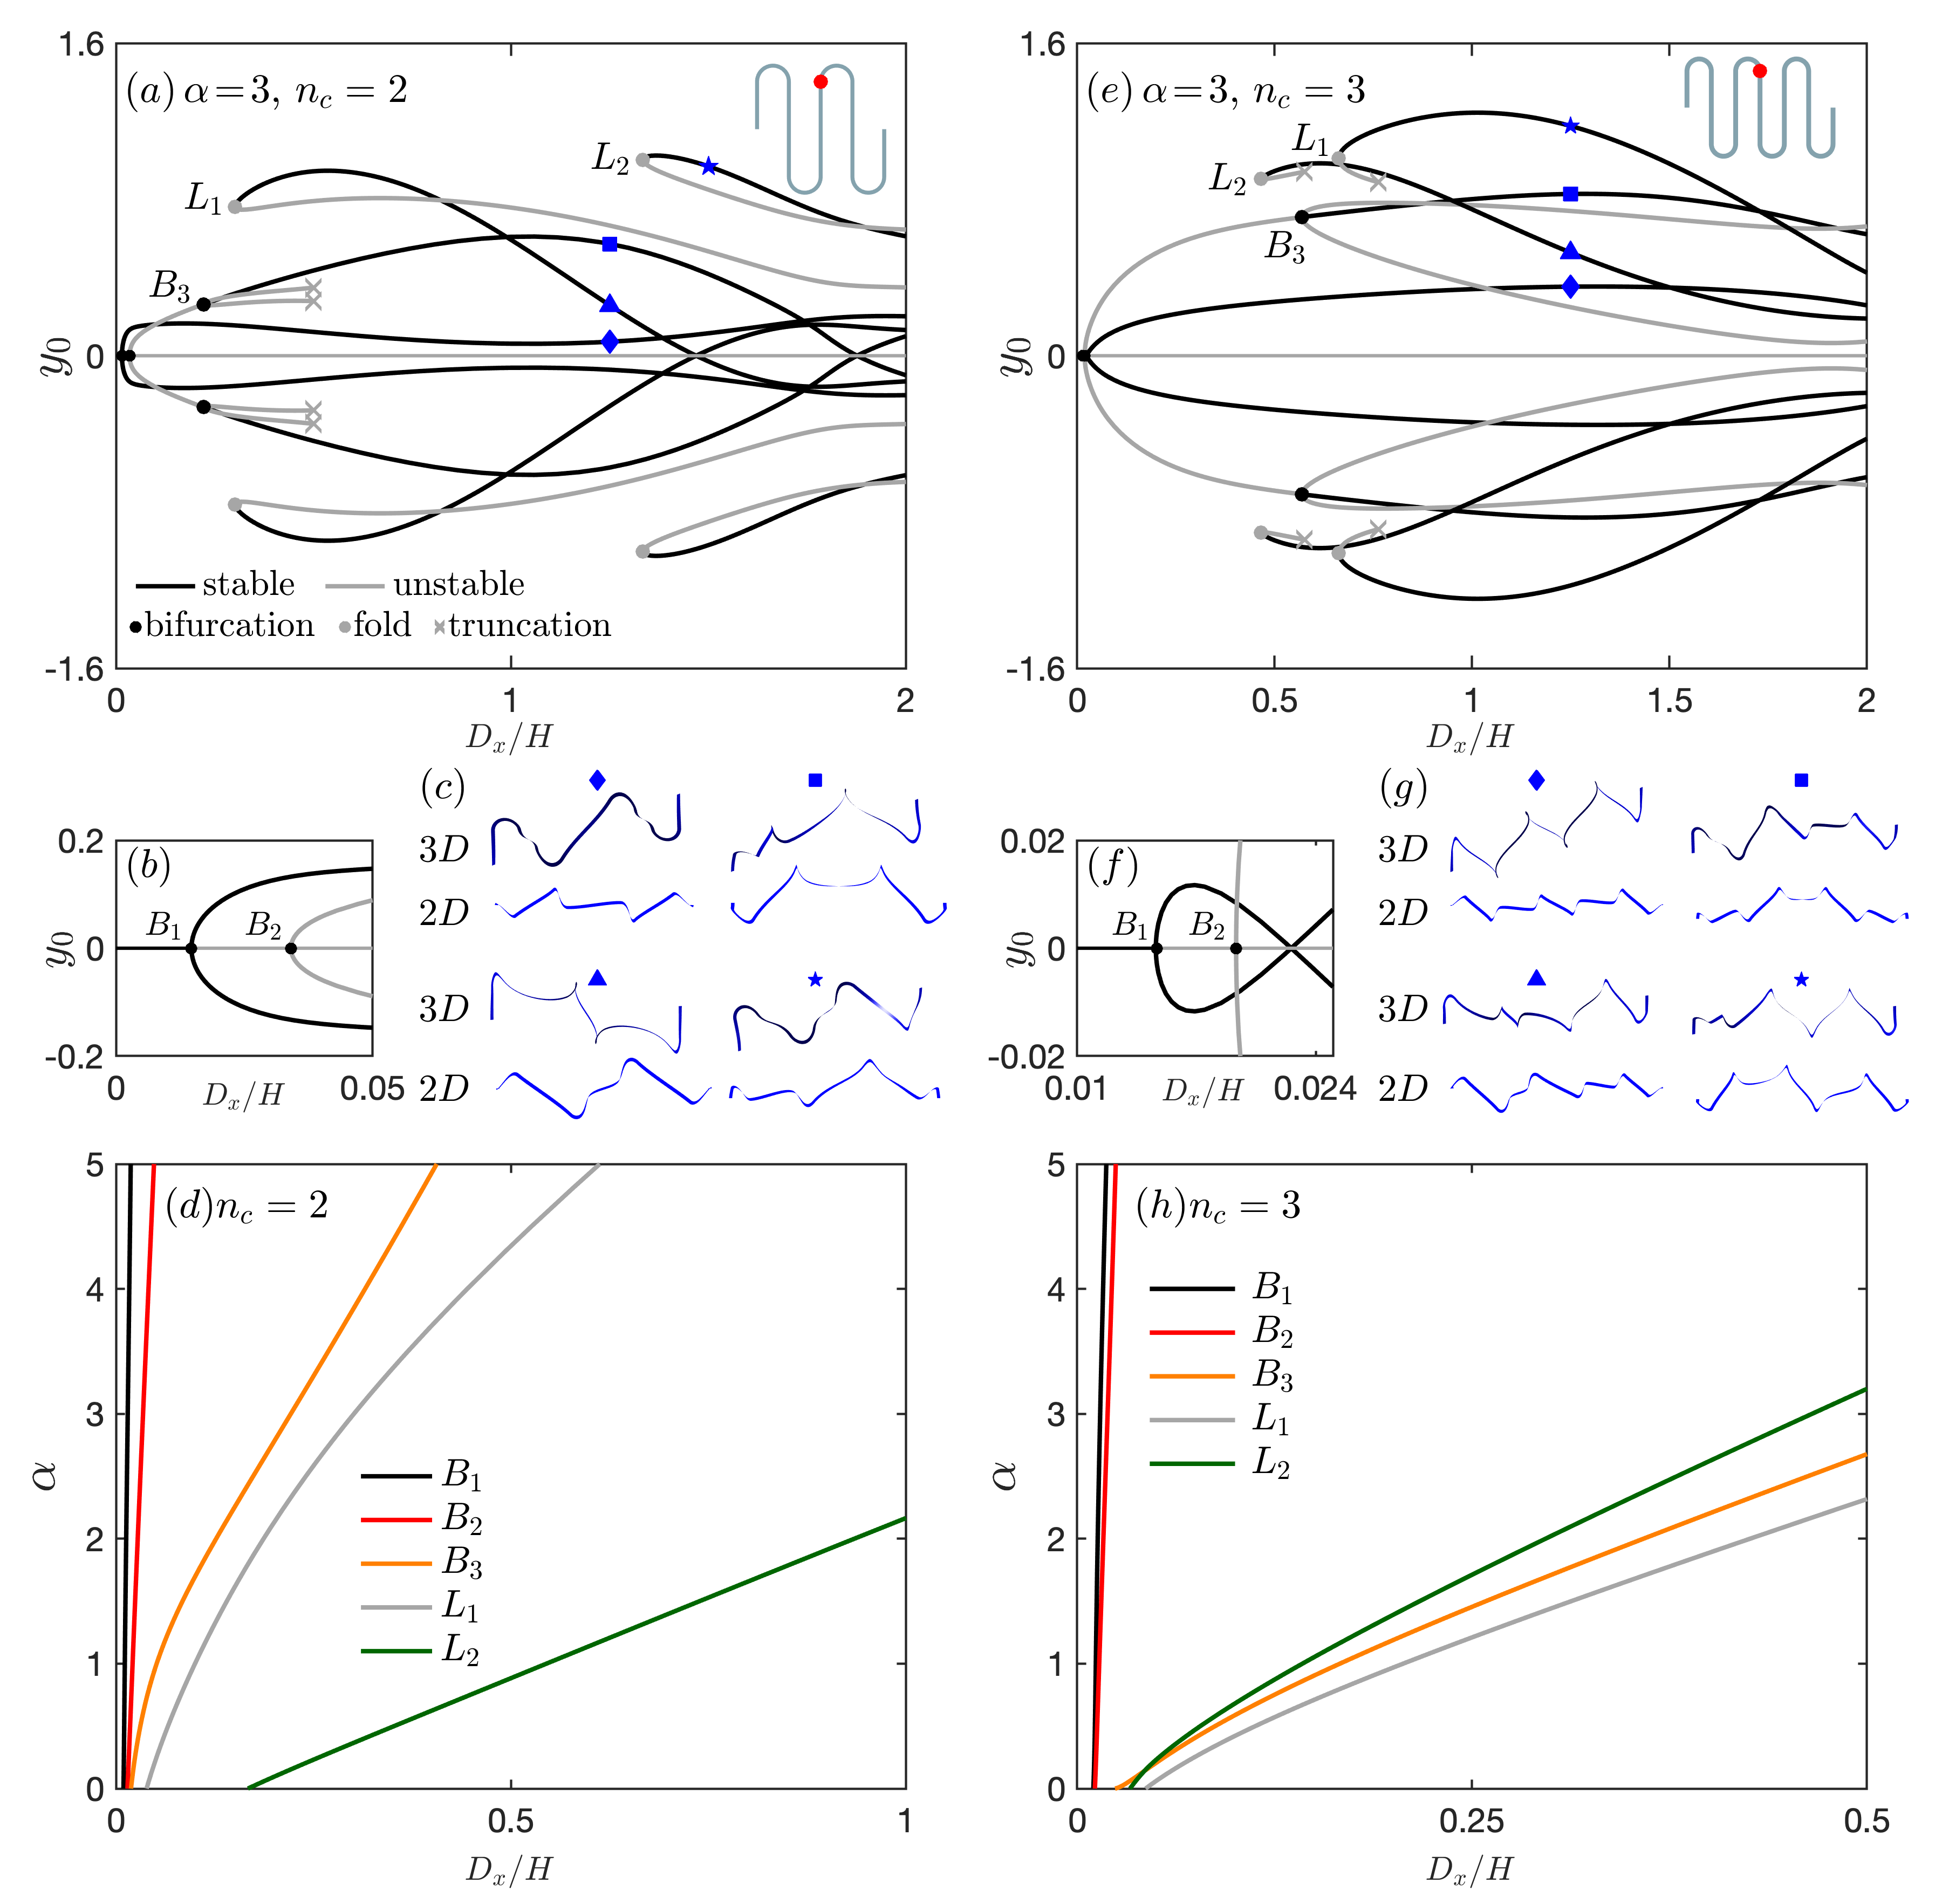
\includegraphics[width=1\linewidth]{SerpentineNc2Nc3Aniso10Phase.png}
	\caption{$n_c=2$,$n_c=3$的蛇形结构的分岔图及其相应分岔点的轨迹,$y_0$表示分岔图(a),(e)中蛇形结构红色标记点的平面外位移($y$方向)。(a) $n_c=2$,$\alpha=3$分岔图。(b) 图(a)的放大图。(c) 图(a)中平衡分支对应的构形。(d) 图(a-b)中分岔点的轨迹图。(e) $n_c=3$,$\alpha=3$分岔图。(f) 图(e)的放大图。(g) 图(e)中平衡分支对应的构形。(h) 图(e-f)中分岔点的轨迹图。}
	\label{fig:SerpentineNc2Nc3Aniso10Phase}
\end{figure}
\section{弹性蛇形条带的多稳态行为}
\subsection{稳态解的获得}
多稳态特性是蛇形结构的另一特点,在某一固定的水平拉伸位移载荷下,蛇形结构往往存在多个稳定的构形。本节通过数值模拟及实验的手段研究了单元数$n_c=1,2,3$的蛇形结构的多稳态行为。从以拉伸位移为延拓参数的分岔图~\ref{fig:SerpentineNc1Aniso10}和~\ref{fig:SerpentineNc2Nc3Aniso10Phase}中可以看出,一部分解与平面分支解$y_0=0$相连,如图~\ref{fig:SerpentineNc1Aniso10}(a),(d)中S模态(~\bluesquare~/~\redsquare~)与M模态(~\Btriangle~/~\Rtriangle~)等对应的平衡分支,为了获得这类解,可将未受拉伸的状态对应的解(力与力矩均为零,结构的空间构形已知)作为参数延拓的初始解。然而部分平衡分支并不与解$y_0=0$相连,如图~\ref{fig:SerpentineNc1Aniso10}(a),(d)和~\ref{fig:SerpentineNc2Nc3Aniso10Phase}(a),(e)中~\Bdiamond~/~\Bstarshape~所标记的平衡分支。对于此类解,无法直接从未受拉伸的解开始延拓得到,为了得到这些孤立平衡分支,需要已知这些孤立分支上的某一点的解作为启动解来获得整条平衡分支。

为了得到这些孤立分支上的一个启动解,一种方法是基于弹性杆静力学平衡方程的方法,通过延拓某一扰动载荷来建立不同的稳定分支之间的联系\cite{Arena_2018,arena2017adaptive}。具体而言,首先从未受载的状态开始,以目标载荷(蛇形条带中,为水平拉伸位移载荷)为延拓参数进行参数延拓,得到特定载荷下的某一稳定构形。然后固定此延拓参数,在该稳定构形上施加某种扰动外力并将该外力作为延拓参数进行延拓,若扰动外力选取得当,所得延拓曲线上存在若干扰动外力为零的点。每一外力为零的点代表着一个平衡解,这样就联系起了在某一固定拉伸载荷下的各个平衡分支。然而对于复杂结构,如蛇形结构,在扰动外力作用下,往往会产生一条复杂的延拓曲线,曲线上存在很多扰动外力为零的点。但这些外力为零的点对应的平衡解往往是非稳定解,无法得到期望的稳定平衡解。

本文采用一种更为有效的方法来寻找稳态解,类似于上述方法,该方法仍通过施加扰动外力的方法寻找稳态解。但不同于上述方法中使用静力学方程进行参数延拓,本方法采用动力学杆模型(这里采用离散弹性杆模型)来进行动力学模拟,在扰动外力下结构直接从某一平衡构形突跳到另一平衡构形。该方法相较于第一种方法具有如下优势:(1)动力学模拟可以捕捉结构的动力学过程,例如结构的突跳过程,使得结构可以直接从某一构形突跳到另一构形上。(2)动力学得到的扰动外力为零的平衡点一定对应稳定解,无需进行额外的稳定性判断。

本节通过下述四个加载过程使得结构从一个稳定构形跳变到另一稳定构形:
\begin{enumerate}
	\item 对结构施加水位移载荷使结构拉伸到目标长度,在阻尼力的作用下,结构会随时间趋于静力学平衡状态。
	\item 在所得稳定的平衡构形上施加扰动力(力矩),当扰动力(力矩)增加到某一临界值时,结构会发生突跳,切换到新的构形上。
	\item 撤除该扰动力,使结构逐渐恢复到未受扰动力的新平衡构形,该平衡构形为新的稳定解。
	\item 在新构形的基础上继续施加扰动,可以得到另一新的构形,如此反复,直到目标构形出现。
\end{enumerate}

对于扰动力(力矩)的确定,包括施加力的位置和具体力的形式(方向、大小),依赖于实验观察。通过实验观察可知,蛇形结构的多稳态表现为结构每一半圆弧段在足够的拉伸位移下,会表现出两种稳定的取向。在多单元蛇形结构中,由于半圆弧段数的增多,结构稳定构形随半圆弧段数增多而急剧增多。因此施加扰动的目的是切换半圆弧段的取向,在扰动力的作用下,半圆弧段从某一取向跳变到另一取向时,蛇形结构的其余部分会随着该切换过程移动到新的位置,达到新的稳态构形。根据实验可知,在半圆弧末端施加扭转力矩,力矩方向始终沿中心线切线方向,可以有效切换相应半圆弧段的取向。对于扰动力矩的大小,本文通过数值计算来确定,结构突跳发生时所需的最小力矩即为所需扰动力矩的大小。以一个双单元蛇形结构($n_c=2$,$\alpha=3$)的突跳为例,如图~\ref{fig:Disturb}所示。从反对称构形(S模态)开始在左起第一个半圆弧末端施加方向沿弧长切线方向的力矩后,该结构从深蓝色条带的构形突跳到半透明蓝色构形。
\begin{figure}
	\centering
	\includegraphics[width=1\linewidth]{Disturb.png}
	\caption{$n_c=2$,$\alpha=3$的蛇形结构在施加扰动前后的平衡构形。其中半透明条带为突跳后的构形,而深蓝色条带为突跳前的构形}
	\label{fig:Disturb}
\end{figure}
\subsection{蛇形条带平衡解的可逆对称性}
在研究蛇形结构的多稳态行为时,利用该结构的对称性可以有效简化分析过程。具体而言,若找到某一稳定平衡解,那么可以通过该结构的对称性直接推断出与其有对称关系的其他稳定平衡解,而无需针对每一稳定平衡解进行动力学模拟。因此,本小节重点研究蛇形结构的对称性。

细长条带结构在两端固支的条件下,往往表现出可逆对称性\cite{starostin2022forceless,van1998lock,champneys1996multiplicity,domokos2001hidden}(reversible symmetry),即同一边界值问题(BVP)的不同的解之间存在一定的关系。

蛇形结构在未加载时的构形呈现出了反对称性,即以结构的几何中心为旋转中心,以$y$轴为旋转轴,做旋转变换,旋转$180^\circ$后构形与原构形重合。因此,若已知某一屈曲构形,那么一定可以通过上述旋转变换,可以得到另外一个满足边界条件的构形。另外,若已知某一构形,那么一定可以通过以$x-z$平面做镜像对称得到另外一满足边界条件的构形。如图~\ref{fig:Groups with four configurations}所示,若在计算过程中得到第一个平衡构形,那么以该构形为基准,通过镜面对称可以得到第二个构形。将第二个构形旋转$180^\circ$可以得到第三个构形,接着对第三个构形进行镜面对称,可以得到第四个构形。因此若已知某一稳态构形,那么一定伴随着其他三个满足边界条件的构形的出现。但需要注意的是,若某一屈曲构形自身具有旋转对称性,那么通过镜面对称变换与通过旋转变换所得构形为同一构形。如图~\ref{fig:reversible pairs}所示,将最左侧构形进行旋转变换或者镜像对称,得到的构形均为第二个构形。因此,可以将蛇形条带的所有屈曲构形分为两类,一类构形本身具有旋转对称性,此类构形总是成对存在,下文将该构形对称为自可逆构形对,另外一类构形自身不具有旋转对称性,此类构形总是成组存在,每组中有四个构形,下文将该类构形组称为平衡构形组。例如,从图~\ref{fig:SerpentineNc1Aniso10}(c)(f)可以看出图~\ref{fig:SerpentineNc1Aniso10}(a)(d)中以~\Brighttriangle/~\Blefttriangle~/~\Rlefttriangle~/~\Rrighttriangle~所标记的四条平衡分支属于同一平衡构形组。以~\HBrighttriangle/~\HBlefttriangle~/~\HRlefttriangle~/~\HRrighttriangle~标记的平衡分支属于另一平衡构形组。以~\bluesquare/~\redsquare~标记的平衡分支属于同一自可逆对。以~\Btriangle/~\Rtriangle~标记的平衡分支属于另一自可逆对。
\begin{figure}
	\centering
	\subcaptionbox{$\alpha=3$,$n_c=2$的一个自可逆构形对\label{fig:reversible pairs}}
	{\includegraphics[width=0.45\linewidth]{reversible pairs.png}}\\
	\subcaptionbox{$\alpha=3$,$n_c=2$的一个平衡构形组\label{fig:Groups with four configurations}}
	{\includegraphics[width=1\linewidth]{Groups with four configurations.png}}
	\caption{$\alpha=3$,$n_c=2$的六个平衡构形}
	\label{fig:reversible pairs and group}
\end{figure}

为了寻找同一自可逆对或同一平衡构形组之内各构形解的关系,本文首先通过施加扰动外力的方法,得到某一平衡构形组(自可逆对)中的所有平衡解,然后观察该组解中各变量之间的变换关系。将所得变换关系代入微分方程来验证该变换关系对任一平衡构形组均有效。对于细长杆结构,若已知该杆的曲率,挠率以及杆内力的三个分量,那么可以唯一确定该弹性杆的构形以及受力情况。因此下面重点研究这六个关键变量之间的关系。

\begin{figure}
	\centering
	\subcaptionbox{~\bluesquare~:$\kappa_1,\kappa_2,\tau$曲线\label{fig:Ra}}
	{\includegraphics[width=0.45\linewidth]{Ra.eps}}
	\subcaptionbox{~\redsquare~:$\kappa_1,\kappa_2,\tau$曲线\label{fig:Rb}}
	{\includegraphics[width=0.45\linewidth]{Rb.eps}}\\
	\subcaptionbox{~\bluesquare~:$N_1,N_2,N_3$曲线\label{fig:R3}}
	{\includegraphics[width=0.45\linewidth]{R3.eps}}
	\subcaptionbox{~\redsquare~:$N_1,N_2,N_3$曲线 \label{fig:Rd}}
	{\includegraphics[width=0.45\linewidth]{Rd.eps}}
	\caption{图~\ref{fig:SerpentineNc1Aniso10}(c)中标记所对应构形的解曲线}
	\label{fig:relation in reversible pair}
\end{figure}
图~\ref{fig:relation in reversible pair}为$\alpha=1.5$,$n_c=1$的蛇形结构的两个互为镜像对称的S模态(共同构成了一个自可逆对)的解曲线,通过观察可知这六个变量具有如下关系:
\begin{equation}
	K: s \rightarrow s, \kappa_{20} \rightarrow \kappa_{20}, \kappa_{1} \rightarrow-\kappa_{1}, \kappa_{2} \rightarrow \kappa_{2}, \tau \rightarrow-\tau, N_{1} \rightarrow N_{1}, N_{2} \rightarrow-N_{2}, N_{3} \rightarrow N_{3}
	\label{eq:K}
\end{equation}
将上述关系式带入原方程,可验证原方程形式保持不变,证明该关系具有普适性。若已知自可逆对中的一个构形,那么根据关系式\eqref{eq:K},可以得到该自可逆对中的另一构形的解。
\begin{figure}
	\centering
	\subcaptionbox{~\Brighttriangle~:$\kappa_1,\kappa_2,\tau$曲线\label{fig:Re}}
	{\includegraphics[width=0.45\linewidth]{Re.eps}}
	\subcaptionbox{~\Rlefttriangle~:$\kappa_1,\kappa_2,\tau$曲线\label{fig:Rf}}
	{\includegraphics[width=0.45\linewidth]{Rf.eps}}\\
	\subcaptionbox{~\Brighttriangle~:$N_1,N_2,N_3$曲线\label{fig:Ri}}
	{\includegraphics[width=0.45\linewidth]{Ri.eps}}
	\subcaptionbox{~\Rlefttriangle~:$N_1,N_2,N_3$曲线 \label{fig:Rj}}
	{\includegraphics[width=0.45\linewidth]{Rj.eps}}
	\subcaptionbox{~\Blefttriangle~:$\kappa_1,\kappa_2,\tau$曲线\label{fig:Rg}}
	{\includegraphics[width=0.45\linewidth]{Rg.eps}}
	\subcaptionbox{~\Rrighttriangle~:$\kappa_1,\kappa_2,\tau$曲线\label{fig:Rh}}
	{\includegraphics[width=0.45\linewidth]{Rh.eps}}\\
	\subcaptionbox{~\Blefttriangle~:$N_1,N_2,N_3$曲线\label{fig:Rk}}
	{\includegraphics[width=0.45\linewidth]{Rk.eps}}
	\subcaptionbox{~\Rrighttriangle~:$N_1,N_2,N_3$曲线 \label{fig:Rl}}
	{\includegraphics[width=0.45\linewidth]{Rl.eps}}
	\caption{图~\ref{fig:SerpentineNc1Aniso10}(c)中标记所对应的构形的解曲线}
	\label{fig:relation in reversible group}
\end{figure}
图~\ref{fig:relation in reversible group}为$\alpha=1.5$,$n_c=1$的蛇形结构的同一平衡构形组中的四个构形相应的解曲线,通过观察可知这六个变量具有如下关系:
\begin{equation}
	\begin{gathered}
		R_{1}: s \rightarrow L-s, \kappa_{20} \rightarrow-\kappa_{20}, \kappa_{1} \rightarrow-\kappa_{1}, \kappa_{2} \rightarrow-\kappa_{2}, \tau \rightarrow-\tau, N_{1} \rightarrow N_{1}, N_{2} \rightarrow N_{2}, N_{3} \rightarrow N_{3} \\
		R_{2}: s \rightarrow L-s, \kappa_{20} \rightarrow-\kappa_{20}, \kappa_{1} \rightarrow \kappa_{1}, \kappa_{2} \rightarrow-\kappa_{2}, \tau \rightarrow \tau, N_{1} \rightarrow N_{1}, N_{2} \rightarrow-N_{2}, N_{3} \rightarrow N_{3} \\
	\end{gathered}
	\label{eq:R1R2}
\end{equation}
将上述关系式带入原方程,可验证原方程形式保持不变,证明该关系具有普适性。若已知一平衡构形组中的一个解,则可以通过式\eqref{eq:R1R2}得到其余构形的解。例如,若第一个构形~\Brighttriangle~已知,那么通过关系式\eqref{eq:R1R2}中$R_1$变换可以得到第二个构形~\Rlefttriangle~相应的解。将第一个构形通过关系式\eqref{eq:R1R2}中$R_2$变换,可以得到构形~\Blefttriangle~对应的解。对于最后一个构形~\Rrighttriangle~,可以对第一个构形进行式\eqref{eq:K}中的$K$变换得到。最后,本处给出关于图~\ref{fig:relation in reversible pair}和图~\ref{fig:relation in reversible group}中$\kappa_2$不连续的原因:在半圆弧与直线段连接处,初始曲率$\kappa_{20}$不连续。
\subsection{蛇形条带的多稳态构形}
本小节给出单元数$n_c=1,2,3$的蛇形结构的稳态构形的数值计算结果以及相应的实验结果。本文首先通过实验观察到某一构形,随后观察可能的施加扰动方法,即通过在哪几个半圆弧端部施加扰动外力,可以从某一已知构形一步步切换到目标构形。然后利用离散弹性杆模型进行相应的动力学模拟来得到数值计算结果。利用该方法可以找到绝大多数稳态构形,但该方法依赖实验来寻找适合的外力类型,另外该方法无法保证可以找到所有稳态构形,即无法找到能量函数的所有局部最小值。因此,本节所列结果只是部分稳态构形,无法保证找到了所有稳定构形。
\begin{figure}[t]
	\centering
	\includegraphics[width=1\linewidth]{ExptsvsSimulations.pdf}
	\caption{不同单元数$n_c$,不同高度$\alpha$的蛇形条带在不同拉伸位移$D_x/H$下,稳定构形的二维俯视图($x-y$平面投影)。黑色背景中构形为实验结果,白色背景对应数值计算结果。(a-f) 单元数$n_c=1$,$\alpha=1.5$的蛇形结构。(g-k) 单元数$n_c=1$,$\alpha=4$的蛇形结构。(l-p) 单元数$n_c$=2,高度$\alpha=3$的蛇形结构。(q-z)单元数$n_c$=3,高度$\alpha=3$的蛇形结构。在每个子图下面$m_n$代表一组$m$个蛇形结构中的$n$个构形}
	\label{fig:ExptsvsSimulations}
\end{figure}

图~\ref{fig:ExptsvsSimulations}展示了不同单元数$n_c$,不同高度$\alpha$的蛇形条带在水平拉伸位移$D_x/H$下的稳定构形的$x-y$方向投影,其中黑色背景为实验结果而白色背景中构形为相应的数值计算结果。在每一个子图下面,用$m_n$代表该构形为一组$m$个构形中的第$n$个构形(顺序$n$为随机排列)。

对于单单元蛇形结构,图~\ref{fig:ExptsvsSimulations}(b-d),(f),(h-j)中的构形表现出了自可逆性(self-reversibility),每一构形为所属自可逆构形对中的一个构形。图~\ref{fig:ExptsvsSimulations}($j_1$),($j_2$)给出了一个自可逆构形对的所有构形。而图~\ref{fig:ExptsvsSimulations}(a),(e),(g),(k)中构形并没有自可逆性,每一个构形均为相应平衡构形组中的一个构形。

对于$\alpha=1.5$,$n_c=1$的蛇形结构,图~\ref{fig:ExptsvsSimulations}(a)对应图~\ref{fig:SerpentineNc1Aniso10}(a)中~\Brighttriangle~所标记的分支;图~\ref{fig:ExptsvsSimulations}(b)中构形为S模态,对应图~\ref{fig:SerpentineNc1Aniso10}(a)中~\bluesquare~所标记的分支;图~\ref{fig:ExptsvsSimulations}(c)为M模态,对应图~\ref{fig:SerpentineNc1Aniso10}(a)中~\Btriangle~所标记的分支;图~\ref{fig:ExptsvsSimulations}(d)对应图~\ref{fig:SerpentineNc1Aniso10}(a)中~\Bdiamond~所标记的分支;图~\ref{fig:ExptsvsSimulations}(e)对应图~\ref{fig:SerpentineNc1Aniso10}(a)中~\HBrighttriangle~所标记的分支;图~\ref{fig:ExptsvsSimulations}(f)对应图~\ref{fig:SerpentineNc1Aniso10}(a)中~\Bstarshape~所标记的分支。

对于$\alpha=4$,$n_c=1$的蛇形结构。图~\ref{fig:ExptsvsSimulations}(g)对应图~\ref{fig:SerpentineNc1Aniso10}(d)中~\Brighttriangle~所标记的分支;图~\ref{fig:ExptsvsSimulations}(h)对应图~\ref{fig:SerpentineNc1Aniso10}(d)中~\Bdiamond~所标记的分支;图~\ref{fig:ExptsvsSimulations}(i)中构形为S模态,对应图~\ref{fig:SerpentineNc1Aniso10}(d)中~\bluesquare~所标记的分支;图~\ref{fig:ExptsvsSimulations}($j_1$),($J_2$)为M模态,对应图~\ref{fig:SerpentineNc1Aniso10}(d)中~\Btriangle~/~\Rtriangle~所标记的分支;图~\ref{fig:ExptsvsSimulations}(k)对应图~\ref{fig:SerpentineNc1Aniso10}(d)中~\HBrighttriangle~所标记的分支。

随着单元的增多,稳态个数及相应的分支曲线也会增多,为了保证分岔图的清晰性,尽管在图~\ref{fig:ExptsvsSimulations}中展示了许多稳态,但多单元蛇形条带分岔图~\ref{fig:SerpentineNc2Nc3Aniso10Phase}并未将这些稳态对应的分岔曲线一一展示。图~\ref{fig:ExptsvsSimulations}(l-p)展示了$(n_c,\alpha)=(2,3)$的蛇形结构在拉伸载荷下的部分稳定构形。图~\ref{fig:ExptsvsSimulations}(l),(m)为自可逆构形,分别对应S模态和M模态。图~\ref{fig:ExptsvsSimulations}($n_1$),($n_2$)为一自可逆构形对。图~\ref{fig:ExptsvsSimulations}($o_1$),($o_2$),($o_3$),($o_4$)给出了同一平衡构形组中的所有构形,而图~\ref{fig:ExptsvsSimulations}($p_1$),($p_2$)为另一个平衡构形组中的其中两个构形。因此,对于$n_c=2$的蛇形条带,本文找到了14个平衡构形。

图~\ref{fig:ExptsvsSimulations}(q-z)展示了$(n_c,\alpha)=(3,3)$的蛇形结构在拉伸载荷下的部分稳定构形。每一构形都属于不同的自可逆构形对或者平衡构形组。其中,图~\ref{fig:ExptsvsSimulations}(q),(r),(v),(w)中的构形分别属于不同的自可逆构形对,其中图~\ref{fig:ExptsvsSimulations}(q)为S模态,图~\ref{fig:ExptsvsSimulations}(r)为M模态。其余的构形分别属于不同的平衡构形组。因此,对于$(n_c,\alpha)=(3,3)$的蛇形结构,这里识别了三十二个平衡构形。

从图~\ref{fig:ExptsvsSimulations}可以看到数值计算的构形与实验结果吻合良好,进一步说明了本文所用计算模型对该结构的有效性,以及实验装置的精确性。

%模板中使用 \pkg{unicode-math} 宏包来配置数学符号,
%
%研究生《写作指南》要求量及其单位所使用的符号应符合国家标准《国际单位制及其应用》(GB 3100—1993)、《有关量、单位和符号的一般原则》(GB/T 3101—1993)的规定,但是与 \TeX{} 默认的美国数学学会(AMS)的符号习惯有所区别。
%
%英文论文的数学符号使用 \TeX{} 默认的样式。论文以中文为主要撰写语言按照国标建议的配置数学字体格式:
%
%\begin{enumerate}
%  \item 大写希腊字母默认为斜体,如
%    \begin{equation*}
%      \Gamma \Delta \Theta \Lambda \Xi \Pi \Sigma \Upsilon \Phi \Psi \Omega.
%    \end{equation*}
%    注意有限增量符号 $\increment$ 固定使用正体,模板提供了 \cs{increment} 命令。
%  \item 小于等于号和大于等于号使用倾斜的字形 $\le$、$\ge$。
%  \item 积分号使用正体,比如 $\int$、$\oint$。
%  \item 行间公式积分号的上下限位于积分号的上下两端,比如
%    \begin{equation*}
%      \int_a^b f(x) \dif x.
%    \end{equation*}
%    行内公式为了版面的美观,统一居右侧,如 $\int_a^b f(x) \dif x$ 。
%  \item
%    偏微分符号 $\partial$ 使用正体。
%  \item
%    省略号 \cs{dots} 按照中文的习惯固定居中,比如
%    \begin{equation*}
%      1, 2, \dots, n \quad 1 + 2 + \dots + n.
%    \end{equation*}
%  \item
%    实部 $\Re$ 和虚部 $\Im$ 的字体使用罗马体。
%\end{enumerate}
%%
%%以上数学符号样式的差异可以在模板中统一设置。
%%另外国标还有一些与 AMS 不同的符号使用习惯,需要用户在写作时进行处理:
%\begin{enumerate}
%  \item 数学常数和特殊函数名用正体,如
%    \begin{equation*}
%      \uppi = 3.14\dots; \quad
%      \symup{i}^2 = -1; \quad
%      \symup{e} = \lim_{n \to \infty} \left( 1 + \frac{1}{n} \right)^n.
%    \end{equation*}
%  \item 微分号使用正体,比如 $\dif y / \dif x$。
%  \item 向量、矩阵和张量用粗斜体(\cs{mathbfit}),如 $\mathbfit{x}$、$\mathbfit{\Sigma}$、$\mathbfit{T}$。
%  \item 自然对数用 $\ln x$ 不用 $\log x$。
%\end{enumerate}
%
%
%
%关于数学符号更多的用法,参考
%\href{http://mirrors.ctan.org/macros/latex/contrib/unicode-math/unicode-math.pdf}{\pkg{unicode-math}}
%宏包的使用说明,
%全部数学符号命的令参考
%\href{http://mirrors.ctan.org/macros/latex/contrib/unicode-math/unimath-symbols.pdf}{\pkg{unimath-symbols}},也可以参考 Stack Overflow 上的答案 \href{https://tex.stackexchange.com/questions/58098/what-are-all-the-font-styles-i-can-use-in-math-mode}{What are all the font styles I can use in math mode?}。
%
%关于量和单位推荐使用
%\href{http://mirrors.ctan.org/macros/latex/contrib/siunitx/siunitx.pdf}{\pkg{siunitx}}
%宏包,
%可以方便地处理希腊字母以及数字与单位之间的空白,
%比如:
%\SI{6.4e6}{m},
%\SI{9}{\micro\meter},
%\si{kg.m.s^{-1}},
%\SIrange{10}{20}{\degreeCelsius}。
%
%
%数学公式可以使用 \env{equation} 和 \env{equation*} 环境。
%注意数学公式的引用应前后带括号,建议使用 \cs{eqref} 命令,比如式\eqref{eq:example}。
%\begin{equation}
%  \frac{1}{2 \uppi \symup{i}} \int_\gamma f = \sum_{k=1}^m n(\gamma; a_k) \mathscr{R}(f; a_k)
%  \label{eq:example}
%\end{equation}
%注意公式编号的引用应含有圆括号,可以使用 \cs{eqref} 命令。
%
%晶体衍射基础的著名公式──布拉格方程:
%\begin{equation}
%  2d\sin\theta=k\lambda, \quad k=1,2,3\ldots
%\end{equation}
%
%\noindent%
%\begin{minipage}{\textwidth}
%  \begin{tabularx}{\textwidth}{@{}l@{~}l@{~——~}X@{}}
%    式中 & $d$ & 晶面间距(nm);\\
%    & $\theta$ & 入射线与晶面的夹角(rad);\\
%    & $\lambda$ & X射线波长(nm)。\\
%    & $k$ & 公式中第一次出现的物理量代号应给予注释,注释的转行应与破折号“——”后第一个字对齐。
%  \end{tabularx}
%\end{minipage}
%
%多行公式尽可能在“=”处对齐,推荐使用 \env{align} 环境。
%\begin{align}
%  a & = b + c + d + e \\
%    & = f + g
%\end{align}
%
%此外需要注意:公式需紧挨段前文字,不可空行,不然会导致公式独立成段,如下\textcolor{red}{\textbf{错误}}效果。公式前文字公式前文字公式前文字公式前文字公式前文字。
%
%\begin{equation}
%  \frac{1}{2 \uppi \symup{i}} \int_\gamma f = \sum_{k=1}^m n(\gamma; a_k) \mathscr{R}(f; a_k)
%\end{equation}
%
%公式后文字公式后文字公式后文字公式后文字公式后文字公式后文字公式后文字公式后文字公式后文字公式后文字公式后文字。\textbf{正确}效果,如下:
%% <- 如需代码上空行需要在前面加上百分号·%
%\begin{equation}
%  \frac{1}{2 \uppi \symup{i}} \int_\gamma f = \sum_{k=1}^m n(\gamma; a_k) \mathscr{R}(f; a_k)
%\end{equation}
%公式后文字公式后文字公式后文字公式后文字公式后文字公式后文字公式后。
%
%\section{数学定理}
%
%定理环境的格式可以使用 \pkg{amsthm} 或者 \pkg{ntheorem} 宏包配置。
%用户在导言区载入这两者之一后,模板会自动配置 \env{thoerem}、\env{proof} 等环境。
%
%\begin{theorem}[Lindeberg--Lévy 中心极限定理]
%  设随机变量 $X_1, X_2, \dots, X_n$ 独立同分布, 且具有期望 $\mu$ 和有限的方差 $\sigma^2 \ne 0$,
%  记 $\bar{X}_n = \frac{1}{n} \sum_{i+1}^n X_i$,则
%  \begin{equation}
%    \lim_{n \to \infty} P \left(\frac{\sqrt{n} \left( \bar{X}_n - \mu \right)}{\sigma} \le z \right) = \Phi(z),
%  \end{equation}
%  其中 $\Phi(z)$ 是标准正态分布的分布函数。
%\end{theorem}
%\begin{proof}
%  Trivial.
%\end{proof}
%
%同时模板还提供了 \env{assumption}、\env{definition}、\env{proposition}、
%\env{lemma}、\env{theorem}、\env{axiom}、\env{corollary}、\env{exercise}、
%\env{example}、\env{remar}、\env{problem}、\env{conjecture} 这些相关的环境。
%
%\section{数学字体}
%
%按照《撰写规范》表达式字体可以采用 Times New Roman、Xits Math 或 Cambria Math(MS Word默认字体)。Cambria Math 缺少部分样式,例如:积分符号设定为 upright 也看起来没有变化。
%
%TeX Gyre Termes Math 字体(Times New Roman的TeX克隆版)样例:
%\makeatletter
%\thu@load@math@font@times
%\begin{equation}
%  \frac{1}{2 \uppi \symup{i}} \int_\gamma f = \sum_{k=1}^m n(\gamma; a_k) \mathscr{R}(f; a_k)
%\end{equation}
%\makeatother
%
%Cambria Math 字体样例:
%\makeatletter
%\thu@load@math@font@cambria
%\begin{equation}
%  \frac{1}{2 \uppi \symup{i}} \int_\gamma f = \sum_{k=1}^m n(\gamma; a_k) \mathscr{R}(f; a_k)
%\end{equation}
%\makeatother
%
%Xits Math 字体样例:
%\makeatletter
%\thu@load@math@font@xits
%\begin{equation}
%  \frac{1}{2 \uppi \symup{i}} \int_\gamma f = \sum_{k=1}^m n(\gamma; a_k) \mathscr{R}(f; a_k)
%\end{equation}
%\thu@load@math@font@cambria
%\makeatother
%
%STIX Math 字体样例:
%\makeatletter
%\thu@load@math@font@stix
%\begin{equation}
%  \frac{1}{2 \uppi \symup{i}} \int_\gamma f = \sum_{k=1}^m n(\gamma; a_k) \mathscr{R}(f; a_k)
%\end{equation}
%\makeatother


% !TeX root = ../sustechthesis-example.tex

\chapter{蛇形结构后屈曲行为的调控}
\section{引言}
上一章研究了蛇形结构的分岔行为以及多稳态行为。该结构在实际应用中,特别是在柔性电路中的应用,往往需要根据实际情况来优化蛇形结构的几何参数。本章将提出一种优化蛇形结构后屈曲行为的方法并给出相应的优化结果。具体而言,通过优化结构的几何参数来实现对结构在后屈曲阶段分岔点位置的控制,从而实现对结构非线性行为的调控。本章首先介绍优化目标函数的设计,以及所用的优化方法及其相应的工具包。随后展示优化结果,结果可分为三部分:对于单单元蛇形结构($n_c=1$)而言,通过优化蛇形结构的厚度分布来调控结构屈曲模态交换的临界高度及相应交换临界载荷。对于双单元蛇形结构($n_c=2$)而言,本章通过优化蛇形结构中各直条带的长度,来实现双单元蛇形结构中的模态交换,并对优化后结构进行详细的分岔分析来阐明在双单元蛇形结构的屈曲模态交换过程中同样存在多重特征值分岔来实现稳定性的交换。最后,对三单元蛇形结构($n_c=3$)而言,本章通过调控不同单元的厚度,来说明通过单元厚度的调节可以有效影响屈曲构形。
\section{结构优化方法}
本节给出用于优化蛇形结构后屈曲行为的目标函数的设计思路,所使用的优化算法以及具体的优化程序。

蛇形结构在临界拉伸载荷下会发生面外屈曲,该临界载荷对应于一个超临界分岔点。进入后屈曲阶段后,一方面,原平面分支上会出现二阶屈曲模态对应的分岔点甚至高阶分岔点。另一方面,在屈曲构形对应的分支上,会有二次分岔点,拐点等特殊分岔点的出现,正是这一系列分岔点的出现,使得蛇形结构展现出了丰富的非线性行为。因此,为了调控蛇形结构的分岔行为,关键在于调控这些分岔点的位置,个数及顺序等信息。本节将会设计合理的目标函数来调控分岔点位置,个数及顺序等信息,以此来实现对结构后屈曲行为的调控。

调控同一平衡分支上不同分岔点的顺序对调控结构后屈曲行为至关重要。例如,蛇形结构的平面平衡分支上存在两个分岔点,其分岔支上对应的构形分别为S模态与M模态。多单元蛇形结构的屈曲构形(S模态)对应第一个分岔支。若通过优化的方法将两个分岔点的顺序进行交换,那么可以使得结构屈曲为M模态。为实现对分岔点顺序的调控,所构造的目标函数应该同时可以控制分岔点出现的个数,识别各个分岔点对应的模态以及控制不同分岔点出现的顺序。这里仍以蛇形条带为例,为了使得S模态以及M模态顺序发生交换,在优化过程中,要尽量避免出现除S模态和M模态对应的两个分岔点之外的第三者出现,即通过合理调控参数延拓的区间,使得在延拓区间内有且仅有两个分岔点。另外,在进行参数延拓过程中,所得信息仅为分岔点的位置,因此需要设计方法来识别各个分岔点对应的模态。

本文采用Melot等\cite{melot:hal-04378993}所提出的构造目标函数的方法,将目标函数分为两部分,分岔度量项(Bifurcation measure term)和误差度量项(Error measure term)。分岔度量项具有如下形式:
\begin{equation}
	\left|\mathcal{T}-\mathcal{P}\right|\Psi\left(\mathbfit{\theta} \right)
	\label{eq:objective function}
\end{equation}
式中,$\mathcal{T}$为目标分岔点集合,$\mathcal{P}$为优化求解器预测得到的分岔点集合。$\left|\mathcal{T}-\mathcal{P}\right|$代表集合$\mathcal{T}-\mathcal{P}$中分岔点个数。该项作为罚函数项,当分岔点个数大于或者小于目标个数时,该项为有限大小,只有当目标个数与实际分岔点个数一致时,该项取得极小值零。

表达式\eqref{eq:objective function}中$\Psi\left(\mathbfit{\theta} \right)$为优化参数$\mathbfit{\theta}$的函数,其目的是用来鼓励分岔点的出现,换言之,在优化过程中出现的分岔点个数越多该项应当越小。为了实现这一效果,一种方式是利用测试函数(test function)$g$来构造$\Psi\left(\mathbfit{\theta} \right)$。

测试函数(test function)\cite{seydel2009practical}为一连续的标量值函数,主要功能是用来在延拓过程中检测各类分岔点的出现。当出现分岔点时,测试函数值会从正到负或从负到正,换言之,测试函数在分岔点处值为0。 若某一固定延拓区间内存在越多分岔点,那么测试函数就会有越多的零点,为了基于测试函数给出$\Psi\left(\mathbfit{\theta} \right)$的定义,这里需要将测试函数进行归一化处理,即
\begin{equation}
	\mathcal{G}(\mathbfit{\theta})=\frac{|g(\mathbfit{\theta})|}{\underset{\mathbfit{R}=\mathbfit{0}}{\max}|g(\mathbfit{\theta})|}
	\label{eq:normalization1}
\end{equation}
式中$\mathbfit{R}=0$为延拓区间,将测试函数用测试函数在延拓区间内的最大值进行归一化,使得函数值$\mathcal{G}(\mathbfit{\theta})$落在区间$\left[0~1\right]$内。为了消除延拓区间长度对$\Psi\left(\mathbfit{\theta}\right)$的影响,用参数延拓区间长度对函数$\mathcal{G}(\mathbfit{\theta})$进行归一化得
\begin{equation}
	\Psi(\mathbfit{\theta})=\frac{\int_{\mathbfit{R}=0} \mathcal{G}(\mathbfit{\theta}) \dif s}{\int_{\mathbfit{R}=0} \dif  s}
	\label{eq:normalization2}
\end{equation}
通过将测试函数经过式\eqref {eq:normalization1},\eqref{eq:normalization2}的两次归一化后,消除了测试函数数值大小与求解问题的关联,与延拓区间大小的关联。当分岔点越多时,函数$\mathcal{G}(\mathbfit{\theta})$对应的零点越多,积分值$\Psi\left(\mathbfit{\theta} \right)$就越小。因此,可以在优化过程中,使优化求解器朝着分岔点增多的方向优化。
	
分岔度量项(bifurcation measure term)作为罚函数项,在优化过程中,出现的分岔点个数与预期出现的个数一致时,该项取得最小值零。而当出现分岔点个数小于预期个数时,由于$\Psi\left(\mathbfit{\theta} \right)$的存在,优化求解器会朝着分岔点增多的方向优化。通过这一分岔度量项实现了对目标分岔点个数的约束,避免了由强制约束分岔点个数而带来的困难和复杂性\cite{doi:10.1137/21M1418708,doi:10.1137/22M1474448}。

目标函数的第二项为误差度量项(Error measure term),主要用来调控优化过程中所出现的分岔点位置。具体表达式可以根据具体的优化目标而设计。在优化过程中,若要规定目标分岔点的位置,那么该误差项可表达为
\begin{equation}
	E=\underset{\mu}{\sum} \left|\pi_{\mu}(\mathbfit{\theta})-\tau_\mu\right|
	\label{eq:Error term1}
\end{equation}
式中$\mu$为目标分岔点的序号,$\pi_{\mu}(\mathbfit{\theta})$为优化过程中第$\mu$个分岔点的位置,而$\tau_\mu$为目标位置。当各个分岔点的位置与目标位置相同时,该误差项取得极小值零。

若要规定两分岔点之间的距离,那么相应的误差度量项为
\begin{equation}
     E=\left|\pi_{1}-\pi_{2}+\mathrm{c} \right|
	\label{eq:Error term2}
\end{equation}
式中$\pi_{1}$,$\pi_{2}$分别为两个分岔点的位置,常数$\mathrm{c}$为两分岔点的目标距离。在实际问题中可以去掉绝对值,通过去绝对值可以在规定两分岔点距离的同时,规定分岔点的前后位置关系。若常数$\mathrm{c}$为正数,那么当该项取得极小值零时,意味着分岔点${\pi_1}$在分岔点${\pi_2}$之前$\left|\mathrm{c}\right|$处。反之,若常数$\mathrm{c}$为负数,意味着分岔点${\pi_1}$在分岔点${\pi_2}$之后$\left|\mathrm{c}\right|$处。

综上所述,该优化问题有如下的形式
\begin{equation}
	\begin{split}
		\text{目标函数} \quad &\left|\mathcal{T}-\mathcal{P}\right|\Psi\left(\mathbfit{\theta} \right)+E\\
		\text{约束} \quad &b_i^l \leqq \theta_i \leqq b_i^u
	\end{split}
\end{equation}
式中,$b_i^l$,$b_i^u$分别为第$i$个优化变量的上下界。当该目标函数值取得极小值零时,达成对蛇形结构的相应优化目标。

定义好上述优化问题后,利用非线性优化工具包NLOPT\cite{NLopt,PRAXIS}并配合分岔分析工具包COCO\cite{dankowicz2013recipes}中的“COLL”工具箱来实现对蛇形结构的优化。非线性优化工具包NLOPT提供了一系列优化方法,由于目标函数中存在分岔点的位置变量,无法求该目标函数的梯度,因此本文采用NLOPT中无梯度优化算法中的Nelder-Mead算法。延拓工具包COCO将在每一优化迭代步中进行参数延拓来得到相应参数下的分岔点位置。此外,在存储延拓结果的数组“bd”中,给出了每一延拓步相应的测试函数值,本文利用这些离散值进行数值积分得到目标函数中的$\Psi\left(\mathbfit{\theta} \right)$。本文主要调控蛇形条带平面平衡分支上的前两个分岔点,分别对应一阶屈曲模态和二阶屈曲模态。因此,在优化过程中目标分岔点个数总为二。具体优化过程如下:

\begin{enumerate}
	\item 以未受载蛇形结构对应的解作为延拓的启动解,以水平拉伸载荷为延拓参数,利用COCO进行解的延拓,并监测延拓区间内分岔点的出现。
	\item 若检测到分岔点的个数为零,可能是由于一阶屈曲模态和二阶屈曲模态态对应的分岔点过于接近,在分岔点检测过程中由于步长较大,错误地跳过了两个分岔点。针对此种情况,应调小延拓过程中的最大步长,重新进行延拓。若分岔点个数仍为零,则说明延拓区间过小,在延拓区间内结构未发生面外屈曲,因此无分岔点出现。对于这类情况,则只计算目标函数中控制分岔点个数的罚函数项$\left|\mathcal{T}-\mathcal{P}\right|\Psi\left(\mathbfit{\theta} \right)$作为该优化参数下目标函数的值,无需计算误差项,直接跳出该迭代步,继续优化过程。
	\item 若检测到分岔点的个数为$1$,则说明延拓区间过小,在延拓区间内只存在一个屈曲模态。针对此类情况同样只计算罚函数项作为目标函数值,跳出该迭代步,继续优化过程。
	\item 若分岔点个数为2,那么分岔点个数满足优化结果,下一步需要判断所得各分岔点对应的模态。具体做法为分别延拓由这两个分岔点分岔出的分岔支,通过分支解来判断相应分支对应的模态。随后计算目标函数值。
	\item 若分岔点个数大于2,则说明延拓区间过大,延拓区间内出现了除S模态和M模态以外其他不稳定模态对应的分岔点。此时只需计算前两个分岔点对应的分支,并判断相应分支的屈曲模态并计算目标函数值。
\end{enumerate}
%本节所述的优化流程不仅可以对超临界分岔点,亚临界分岔点进行调控。相同的优化流程也可以用于对拐点等其他特殊分岔点的调控。例如通过调控拐点
\section{调控结果分析}
\subsection{单单元蛇形结构的屈曲模态调控}
上一章结果表明,对于单单元蛇形条带($n_c=1$),其屈曲模态会随着结构高度$\alpha$的不同展现出不同的屈曲模态(S模态以及M模态),本小节将通过对结构几何参数进行优化,来调控模态交换发生的临界高度。在保持结构对称性的前提下,以蛇形结构的两端直线段厚度$t_1$及中间直线段厚度$t_2$为优化参数。如图~\ref{fig:OPT1}所示,在优化过程中,保持蓝色半圆弧段的宽厚比$w/t=10$,通过调节绿色段的厚度$t_1$以及红色段厚度$t_2$来改变相应段的宽厚比(优化后的宽厚比分别为$w/t_1$和$w/t_2$)来实现对临界高度的调控。此外,在调控临界交换高度的同时可以调控在该高度下蛇形结构的临界屈曲载荷。为实现这一优化目标,目标函数中误差度量项应为
\begin{equation}
	E=\left|\pi_{1}-\tau\right|+\left|\pi_{2}-\tau\right|
\end{equation}
式中$\pi_{1},\pi_{2}$分别为一阶屈曲模态与二阶屈曲模态对应的分岔点位置,当两分岔点趋于同一值$\tau$时,目标函数取得极小值零,所得优化参数使得蛇形结构在固定高度处发生屈曲模态交换,且对应的临界屈曲载荷为$\tau$。在优化过程中,允许的厚度调节范围是相比原厚度减小一半或增厚一倍,即$5<w/t_1,w/t_2<20$
下面通过表格列举优化结果。

\begin{figure}
	\centering
	\includegraphics[width=0.25\linewidth]{OPT1.eps}
	\caption{单单元蛇形结构,相同颜色的条带优化过程中保持厚度相同}
	\label{fig:OPT1}
\end{figure}
、
\begin{table}
	\centering
	\caption{优化后的蛇形条带($n_c=1$)的厚度}
	\begin{tabular}{ll}
		\toprule
		临界交换高度及交换载荷          & 优化后宽厚比$w/t$   \\
		\midrule
		$\alpha=3,\pi_{\mathrm{cr}}=0.03$   & $w/t_1=11.86,\quad  w/t_2=15.00$ \\
		$\alpha=3,\pi_{\mathrm{cr}}=0.04$   & $w/t_1=9.90,\quad~~ w/t_2=13.06$    \\
		$\alpha=2,\pi_{\mathrm{cr}}=0.03$   & $w/t_1=11.66,\quad w/t_2=11.75$    \\
%		$\alpha=2,\pi_{\mathrm{cr}}=0.04$   & $w/t_1=,\quad w/t_2=$  \\
		\bottomrule
	\end{tabular}
	\label{tab:three-line}
\end{table}
\subsection{双单元蛇形结构的屈曲模态调控}
对单元数$n_c=2$的蛇形结构屈曲后同时具有S模态和M模态,如图~\ref{fig:OPT_1}所示。不同于单单元蛇形结构,多单元蛇形结构在不同结构高度$\alpha$下,S模态对应的临界载荷总小于M模态出现所需的最小载荷。因此,双单元蛇形结构发生平面失稳后总表现为S模态。本小节的优化目标为:在保持结构对称性的前提下,通过优化不同直线型条带的高度,实现S模态与M模态的顺序交换,即M模态出现所需的最小位移载荷小于S模态。
\begin{figure}
	\centering
	\subcaptionbox{双单元蛇形结构的S模态的$x-y$平面投影图(上)与M模态投影图(下)\label{fig:OPT_1}}
	{\includegraphics[width=0.45\linewidth]{OPT_1.png}}
	\subcaptionbox{优化后双单元蛇形结构构形\label{fig:OPT_Schematics}}
	{\includegraphics[width=0.3\linewidth]{OPT_Schematics.eps}}\\
	\caption{未优化前双单元蛇形结构的S模态和M模态以及优化后双单元蛇形结构}
	\label{fig:OPT_Intro}
\end{figure}

本处优化参数为直线型条带的无量纲高度,分别为图~\ref{fig:OPT_Schematics}中左起第一段直条带无量纲长度$l_3/l_1$和第二段直线条带无量纲长度$l_2/l_1$,为了保持结构的反对称性不变,最后一段直条带无量纲长度为$l_3/l_1$,倒数第二段直条带为$l_2/l_1$。最中间直条带的长度由其他直条带长度唯一确定,长度为$2\left(l_2-l_3\right)$。另外,为使优化求解器可以根据优化过程中出现的分岔点数量来自主决定下一优化步所需延拓区间的长度,这里将延拓区间的长度设优化参数,以保证在最终的优化结果中,延拓区间内只存在两个分岔点,对应S模态和M模态。综上所述,本优化问题的优化参数为三个,分别是第一段直条带长度$\alpha_2$和第二段直条带长度$\alpha_1$,以及延拓区间长度。

上一节指出在每一优化步中,参数延拓完成后需要判断所得分岔点对应的屈曲模态。为了区分分岔点对应的屈曲模态,分别向分岔支进行延拓任意固定步数(本文延拓$50$步),取出第$50$步计算得到的平衡解来给出图~\ref{fig:OPT_Schematics}中红色标注点$y$方向的位移,分别为$y_0$,$y_1$。该两点为蛇形结构上互为反对称的两点,从图~\ref{fig:OPT_1}中可以看出,对于S模态而言,结构上互为反对称的两点$y$方向位移大小相同,方向相反。而M模态上互为反对称的两点$y$方向位移,大小相同方向同向。因此可通过位移$y_1$,$y_2$之和来区分不同模态,若$y_1+y_2>0$,则所对应模态为M模态,若$y_1+y_2=0$,那么对应的模态为S模态。

为了实现双单元结构屈曲模态的交换,目标函数的误差度量项应为
\begin{equation}
	E=\pi_{1}-\pi_{2}+\mathrm{c}
	\label{eq:Error term2}
\end{equation}
式中$\pi_{1}$,$\pi_{2}$分别为M模态和S模态对应的分岔点位置。当两个分岔点位置相同时,即$\pi_{1}-\pi_{2}=0$,对应的优化参数为临界交换参数。通过设置一个很小的正数$\mathrm{c}$,用以确保当优化参数取得极小值零时,蛇形结构的一阶屈曲模态为M模态。

优化结果如图~\ref{fig:Phase_RB}所示,该图给出了在不同无量纲高度$\alpha_1$,$\alpha_2$组合下,双单元蛇形结构的一阶屈曲模态,若优化参数$\alpha_1$,$\alpha_2$落入红色区域,那么优化后蛇形结构的一阶屈曲模态为M模态,即相比于优化前,屈曲模态发生了交换;若优化参数$\alpha_1$,$\alpha_2$落入蓝色区域,那么其一阶屈曲模态仍为S模态。图~\ref{fig:Phase_RB}中红蓝区域的交界为临界参数,该交界上两分岔点重合。
\begin{figure}
	\centering
	\includegraphics[width=1\linewidth]{Phase_RB.png}
	\caption{优化后蛇形结构的参数$\alpha_1,\alpha_2$落入蓝色区域,其一阶屈曲模态为S模态;红色区域为M模态}
	\label{fig:Phase_RB}
\end{figure}

为了研究优化后蛇形结构的模态交换过程,本文以固定$\alpha_2=1$为例,研究蛇形结构屈曲模态随$\alpha_1$变化的交换过程。根据优化结果可知,$\alpha_1=4.54$为临界交换点,若$\alpha_1>4.54$,那么优化后结构的一阶屈曲模态为M模态,若$\alpha_1<4.54$,那么优化后结构的一阶屈曲模态为S模态。为了得到结构在该参数下详细的模态交换过程,这里在临界交换点附近分别取$\alpha_1=4,4.75,5$三个参数,来绘制相应的分岔曲线,如图~\ref{fig:OPT2_Bifurcation}(a-c)所示,分别代表屈曲模态交换前,分岔点位置发生交换而稳定性未完全交换,屈曲模态完全交换后的分岔曲线。
\begin{figure}
	\centering
	\subcaptionbox{$\alpha_1=4$下的分岔图\label{fig:OPT2_1}}
	{\includegraphics[width=0.495\linewidth]{OPT2_1.eps}}
	\subcaptionbox{$\alpha_1=4.75$下的分岔图\label{fig:OPT2_2}}
	{\includegraphics[width=0.495\linewidth]{OPT2_2.eps}}\\
	\subcaptionbox{$\alpha_1=5.75$下的分岔图\label{fig:OPT2_3}}
    {\includegraphics[width=0.495\linewidth]{OPT2_3.eps}}
    \subcaptionbox{分岔图(a-c)中分岔点随$\alpha_1$的轨迹\label{fig:OPT2_4}}
    {\includegraphics[width=0.495\linewidth]{OPT2_4.eps}}\\
    \subcaptionbox{不同$\alpha_1$下一阶屈曲模态(左)及二阶屈曲模态(右)\label{fig:OPT2_R}}
    {\includegraphics[width=1\linewidth]{OPT2_R.eps}}    
    \caption{$\alpha_2=1$,不同$\alpha_1$	​
    	取值下双单元蛇形结构的分岔图,包括分岔点的轨迹以及不同参数下的一阶屈曲模态和二阶屈曲模态}	
	\label{fig:OPT2_Bifurcation}
\end{figure}

图~\ref{fig:OPT2_Bifurcation}的分岔图中,分岔点$B_1$,$B_2$分别对应S模态和M模态的分岔点,图~\ref{fig:OPT2_1}中,分岔点$B_1$在分岔点$B_2$之前,因此结构失稳后首先出现S模态。而分岔点$B_2$的分岔支(对应M模态)在分岔点$B_3$之前为不稳定解,在分岔点$B_3$之后,M模态和S模态同时存在。图 ~\ref{fig:OPT2_2}为$\alpha_1=4.75$的分岔图,该分岔图中分岔点$B_2$先于分岔点$B_1$,当达到失稳临界载荷时,结构会屈曲为M模态。M模态对应的平衡解在经过超临界分岔点$B_4$变为非稳定解,但随后经过亚临界分岔点$B_3$后重新恢复为稳定平衡解。在平面解分支($y_0=0$)上分岔点$B_2$之后存在分岔点$B_1$,从该分岔点分岔出一对不稳定的平衡分支,该分岔支在经过超临界分岔点$B_5$之后变为稳定分支,对应稳定的S模态。类似图~\ref{fig:SerpentineNc1Aniso10Phase}中$\alpha=2.346$,$n_c=1$的蛇形结构的分岔曲线,分岔点$B_4$和$B_5$共同构成一个闭合的环。如图~\ref{fig:OPT2_3}所示,随着$\alpha_1$的进一步增大,分岔点$B_4$和$B_5$相互融合,使得M模态对应的整个分岔支变为稳定分支。

图~\ref{fig:OPT2_4}为分岔图中各分岔点随$\alpha_1$的轨迹图,通过轨迹图可以确定模态交换的临界$\alpha_1=4.541$,同时可以看出二次分岔点$B_4$的在临界$\alpha_1$时出现,使得两个屈曲模态的平衡分支的稳定性发生了交换。从以上分岔分析可知,优化后蛇形结构的模态交换同样伴随着多重特征值分岔的出现,多重特征值分岔引发二次分岔点$B_4$,$B_5$的出现,使得S模态与M模态的平衡分支发生了稳定性交换。图~\ref{fig:OPT2_R}展示了$\alpha_1=4,D_x/H=1.5$以及$\alpha_1=5,D_x/H=1.5$对应的一阶屈曲模态(左起第一第三构形为一阶屈曲模态)和二阶屈曲模态(左起第二第四构形为二阶屈曲模态),进一步说明了大于临界$\alpha_1$的蛇形结构其一阶屈曲模态为M模态,小于临界$\alpha_1$的蛇形结构其一阶屈曲模态为S模态。
\subsection{三单元蛇形结构的屈曲模态调控}
本小节以三单元蛇形结构为例,来说明通过改变蛇形结构不同单元的厚度,可以有效调控其屈曲构形。具体而言,在后屈曲阶段,通过调控单元厚度可以抑制某些单元的形变,也可以鼓励某一单元发生更大的形变,这为蛇形结构在实际应用中的设计提供了重要的思路。

图~\ref{fig:OPT3}为单元厚度调节后的蛇形条带($n_c=3$)的屈曲构形及分岔图。在调节厚度的过程中,保持条带的宽度不变,通过改变条带厚度来改变条带截面的宽厚比。图~\ref{fig:OPT_NC3_1}中第$\rom{1}$行展示了蛇形单元在五种情况下的厚度分布。在第一种情况下,整个条带的厚度均匀分布,宽厚比$w/t$为$10$。在后面的几种蛇形条带中,总有一个单元宽厚比不为$10$,具体而言,用蓝色表示的单元宽厚比默认为$10$,而红色表示的单元宽厚比$w/t$等于$8$或者$12.5$。图~\ref{fig:OPT3_1}和图~\ref{fig:OPT3_2}分别为第一个单元宽厚比$w/t=12.5,8$的蛇形结构的分岔图。分岔图中平衡分岔支上标记点处的屈曲构形的二维投影如图~\ref{fig:OPT_NC3_1}中第(b-c)列所示。以图~\ref{fig:OPT_NC3_1}中第(a)列的原构形为基准,第一个单元厚度增大后,如图~\ref{fig:OPT_NC3_1}中第(c)列所示,该单元屈曲后的面外形变被抑制;在减薄第一个单元厚度的情况下,如图~\ref{fig:OPT_NC3_1}中第(b)列所示,该单元的面外变形被放大。分岔图~\ref{fig:OPT3_1}和图~\ref{fig:OPT3_2}表明,当载荷超过临界值$B_1$时,结构屈曲为S模态(~\blacksquare~/~\blackdiamond~),而M模态(~\bltriangle~/~\Rtriangle~)对应的平衡分支不与平面解相连,该分支在拐点$L_1$之后变为稳定解。对蛇形结构($n_c=3$)的第一个单元厚度调控后,整个结构失去了反对称性,即破坏了可逆对称性,关系式\eqref{eq:R1R2}失效。
\begin{figure}
	\centering
	\subcaptionbox{第一个蛇形单元$w/t=12.5$下的分岔图\label{fig:OPT3_1}}
	{\includegraphics[width=0.495\linewidth]{OPT3_1.eps}}
	\subcaptionbox{第一个蛇形单元$w/t=8$下的分岔图\label{fig:OPT3_2}}
	{\includegraphics[width=0.495\linewidth]{OPT3_2.eps}}\\
	\subcaptionbox{第二个蛇形单元$w/t=12.5$\label{fig:OPT3_3}}
	{\includegraphics[width=0.495\linewidth]{OPT3_3.eps}}
	\subcaptionbox{第二个蛇形单元$w/t=8$时的分岔图\label{fig:OPT3_4}}
	{\includegraphics[width=0.495\linewidth]{OPT3_4.eps}}\\
	\subcaptionbox{厚度优化后的结构屈曲构形。红色表示的单元为厚度经过调节后的单元\label{fig:OPT_NC3_1}}
	{\includegraphics[width=1\linewidth]{OPT_NC3_1.png}}
	\caption{厚度优化后$n_c=3$的蛇形结构的屈曲构形及分岔图}	
	\label{fig:OPT3}
\end{figure}

图~\ref{fig:OPT3_3}和图~\ref{fig:OPT3_4}为调控中间单元厚度后的蛇形结构($n_c=3$)的分岔图,调控后第二个单元的宽厚比$w/t$分别为$12.5$和$8$。这种情形下,调控后的蛇形结构仍然保持反对称性,因此可逆对称性的关系式\eqref{eq:R1R2}仍然满足,平衡构形仍成对(自可逆对)或成组(平衡构形组)存在。在分岔点$B_1$后,调控后的蛇形结构发生面外屈曲,屈曲模态为S模态,平面平衡分支上第二个分岔点$B_2$分岔出一对不稳定的平衡分支,当该分岔支穿过$B_3$时,变为稳定解,对应M模态。从图~\ref{fig:OPT_NC3_1}中第(d-e)列可以看出增大厚度会抑制屈曲形变,减小厚度会放大屈曲形变。



% !TeX root = ../sustechthesis-example.tex

\chapter{English and $\text{lower-case}$ Example}

If your supervisor is a foreign resident, or if your supervisor or defense committee specifically allows writing in English, the thesis may be written in English as the primary language. Please check with your supervisor or department secretary to confirm if you can write in English.

\section{Reference guide}

Writing in English still requires the Chinese reference standard GB/T 7714-2015.



% 参考文献
\bibliography{ref/refs}  % 参考文献使用 BibTeX 编译
% \printbibliography       % 参考文献使用 BibLaTeX 编译(兼容性不佳,不太推荐)

% 附录
\appendix
% % !TeX root = ../sustechthesis-example.tex

\chapter{补充内容}

附录是与论文内容密切相关、但编入正文又影响整篇论文编排的条理和逻辑性的资料,例如某些重要的数据表格、计算程序、统计表等,是论文主体的补充内容,可根据需要设置。


\section{图表示例}

\subsection{图}

附录中的图片示例(图~\ref{fig:appendix-figure})。

\begin{figure}
  \centering
  \includegraphics[width=0.6\linewidth]{example-image-a.pdf}
  \caption{附录中的图片示例}
  \label{fig:appendix-figure}
\end{figure}


\subsection{表格}

附录中的表格示例(表~\ref{tab:appendix-table})。

\begin{table}
  \centering
  \caption{附录中的表格示例}
  \begin{tabular}{ll}
    \toprule
    文件名          & 描述                         \\
    \midrule
    sustechthesis.dtx   & 模板的源文件,包括文档和注释 \\
    sustechthesis.cls   & 模板文件                     \\
    thuthesis-*.bst & BibTeX 参考文献表样式文件    \\
    thuthesis-*.bbx & BibLaTeX 参考文献表样式文件  \\
    thuthesis-*.cbx & BibLaTeX 引用样式文件        \\
    \bottomrule
  \end{tabular}
  \label{tab:appendix-table}
\end{table}


\section{数学公式}

附录中的数学公式示例(公式\eqref{eq:appendix-equation})。
\begin{equation}
  \frac{1}{2 \uppi \symup{i}} \int_\gamma f = \sum_{k=1}^m n(\gamma; a_k) \mathscr{R}(f; a_k)
  \label{eq:appendix-equation}
\end{equation}


\section{源代码}

附录中的代码示例:
% 代码\ref{lst:appendix-sample-code-minted},
代码\ref{lst:appendix-sample-code-listings}。

% \begin{listing}[!ht]
% \caption{C++ 代码示例(使用 \pkg{minted} 高亮)}
% \label{lst:appendix-sample-code-minted}
% \begin{minted}[xleftmargin=20pt,linenos]{cpp}
% #include <cstdio>
% #include <cstdlib>
% #include <iostream>
% using namespace std;
% unsigned short i;
% int main() {
%   for (i = 0; i <= 5; i++) {
%     // whatever
%   }
%   return 0;
% }
% \end{minted}
% \end{listing}

\noindent% 取消 minipage 的缩进
\begin{minipage}{\linewidth}
\begin{lstlisting}[language=java,caption={Java 代码示例(使用 \pkg{listings} 高亮)},xleftmargin=20pt,label={lst:appendix-sample-code-listings}]
class HelloWorldApp {
    public static void main(String[] args) {
        System.out.println("Hello World!"); // Display the string.
        for (int i = 0; i < 100; ++i) {
            System.out.println(i);
        }
    }
}
\end{lstlisting}
\end{minipage}

\section{伪代码}

附录中的伪代码示例(算法\ref{algo:appendix-sample-pseudocode})。

\begin{algorithm}
  \caption{Simulation-optimization heuristic}
  \label{algo:appendix-sample-pseudocode}
  \KwData{current period $t$, initial inventory $I_{t-1}$, initial capital $B_{t-1}$, demand samples}
  \KwResult{Optimal order quantity $Q^{\ast}_{t}$}
  $r\leftarrow t$\;
  $\Delta B^{\ast}\leftarrow -\infty$\;
  \While{$\Delta B\leq \Delta B^{\ast}$ and $r\leq T$}{$Q\leftarrow\arg\max_{Q\geq 0}\Delta B^{Q}_{t,r}(I_{t-1},B_{t-1})$\;
  $\Delta B\leftarrow \Delta B^{Q}_{t,r}(I_{t-1},B_{t-1})/(r-t+1)$\;
  \If{$\Delta B\geq \Delta B^{\ast}$}{$Q^{\ast}\leftarrow Q$\;
  $\Delta B^{\ast}\leftarrow \Delta B$\;}
  $r\leftarrow r+1$\;}
\end{algorithm}


\end{document}
